\begin{appendix} %Anhang
\section{Projektvereinbarung}	
\begin{figure}[ht!]
	\centering
	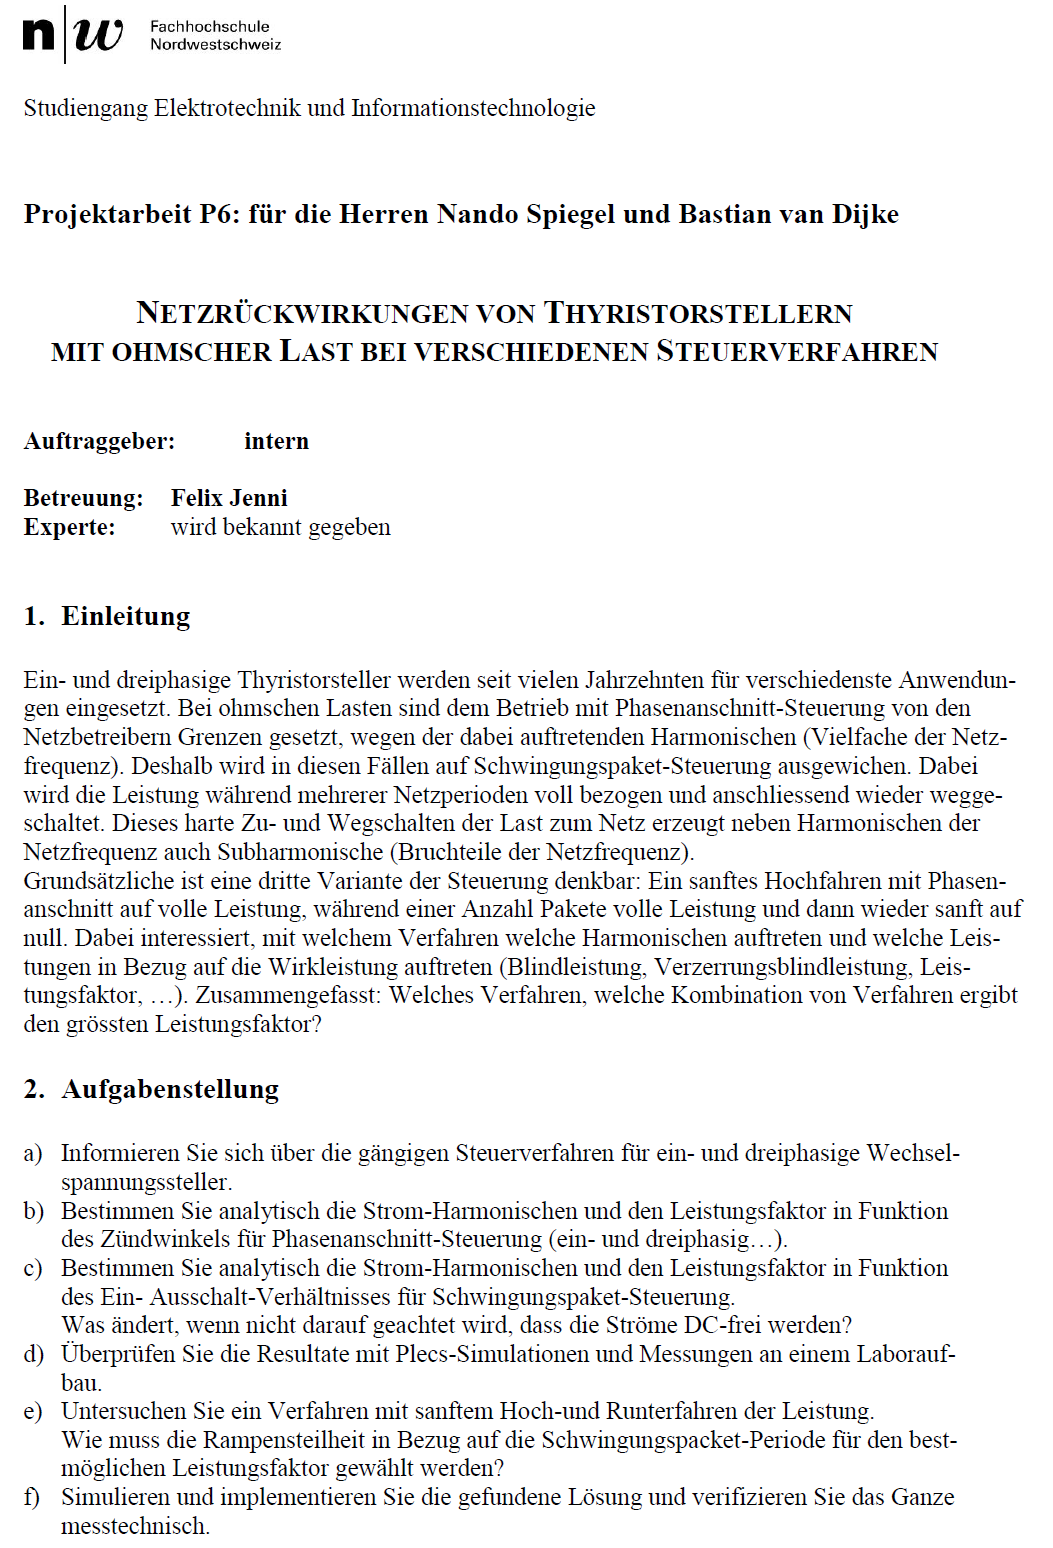
\includegraphics[width=0.95\textwidth]{Projekt_1.png}	
\end{figure}
\newpage
\begin{figure}[ht!]
	\centering
	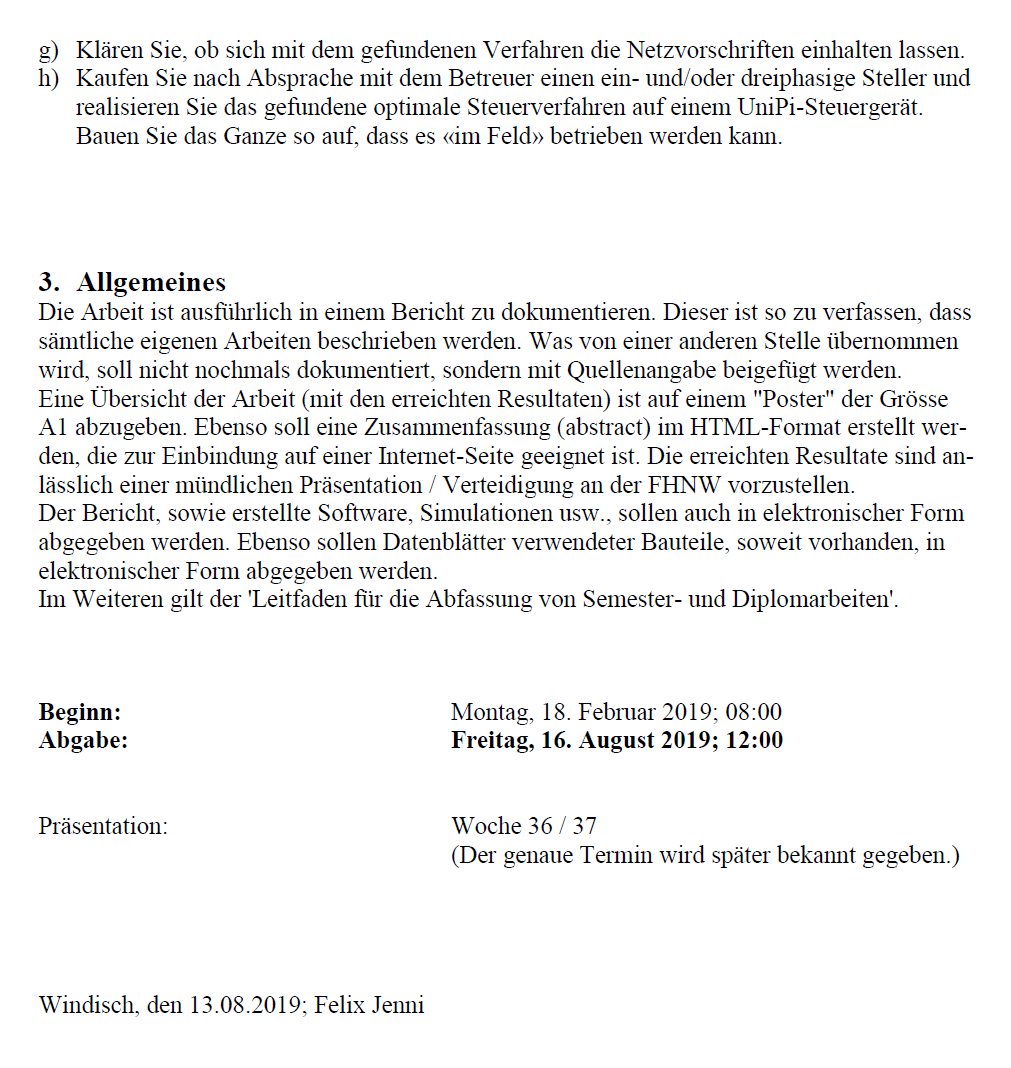
\includegraphics[width=0.95\textwidth]{Projekt_2.png}	
\end{figure}
\newpage
\section{Code}
\subsection{Matlab Berechnungen}
\subsection*{Leistungsfaktor}\label{sec:Leistungsfaktor_Berechnung}
\lstinputlisting{appendix/code/Leistungsfaktor.m}

\subsection*{Phasenanschnitt}\label{sec:Phasenanschnitt_Berechnung}
\lstinputlisting{appendix/code/FTT_Phasenanschnitt_final.m}

\subsection*{Schwingungspaket}\label{sec:Schwingungspaket_Berechnung}
\lstinputlisting{appendix/code/Schwingungspaketsteuerung_final.m}

\subsection*{Fourieranalyse von Hand}\label{sec:Fourieranalyse_Berechnung}
\lstinputlisting{appendix/code/Fourieranalyse_phasenanschnitt_final.m}

\subsection*{Trapez Funktion}\label{sec:Trapez_Berechnung}
\lstinputlisting{appendix/code/Trapez_funktion_final.m}

\subsection*{Leistungsfaktor der Messungen}\label{sec:Leistungsfaktor_Messungen}
\lstinputlisting{appendix/code/Leistungsfaktor_Messungen.m}

\subsection*{Spannungssignale mit FFT}\label{sec:Spannungen_Messungen}
\lstinputlisting{appendix/code/Berechnung_FFT_Widerstand.m}

\subsection*{Stromsignale mit FFT}\label{sec:Stroeme_Messungen}
\lstinputlisting{appendix/code/Berechnung_FFT_Stroeme_Widerstand.m}


\newpage
\subsection{Arduino-Programm}

\subsection*{Phasenanschnittsteuerung}
\begin{lstlisting}[basicstyle=\tiny,style=myArduino]
const int Switch_PO = 3;	// Output fuer den EIN- & AUSSCHALTER
const int Controll_P = 2;	// Output fuer Steuersignal
const int Switch_PI = 5;	// Input fuer den EIN- & AUSSCHALTER
int buttonState = 0;	// Zustand Schalter auf 0


void setup() {
pinMode (Switch_PO, OUTPUT);	// Schalter auf Output
pinMode (Controll_P, OUTPUT);	// PWM auf Output
pinMode (Switch_PI, INPUT_PULLUP);	// Schalter Eingang
}

void loop() {
analogWrite(Controll_P, 127); //Zuendwinkel ausgeben
}
\end{lstlisting}


\subsection*{Schwingungspaketsteuerung}
\begin{lstlisting}[basicstyle=\tiny,style=myArduino]
const int Switch_PO = 3;	// Output fuer den EIN- & AUSSCHALTER
const int Controll_P = 2;	// Output fuer Steuersignal
const int Switch_PI = 5;	// Input fuer den EIN- & AUSSCHALTER
int buttonState = 0;	// Zustand Schalter auf 0
int anzahl_Schwinwungspakete = 5;	// Anzahl Schwingungspakete

void setup() {
pinMode (Switch_PO, OUTPUT);	// Schalter auf Output
pinMode (Controll_P, OUTPUT);	// PWM auf Output
pinMode (Switch_PI, INPUT_PULLUP);	// Schalter Eingang
}

void loop() {
	buttonState =! digitalRead(Switch_PI);	// Da Pullup wird das Signal negiert
	if(buttonState == HIGH){	// if-Schleife falls Zustand Schalter auf EIN
		digitalWrite(Controll_P, HIGH);	// Auf High schalten um Zuendwinkel von 0 Grad zu erreichen (Volle Leistung)
		delay(800);	// Warten waehrend volle Leistung
		digitalWrite(Controll_P, LOW);	// Auf Low schalten um Zuendwinkel von 180 Grad zu erreichen (Keine Leistung)
		delay(200);// Genug Zeit zwischen den Paketen weil sonst wird eine Spannung von 0V nicht erreicht     
	}
}
\end{lstlisting}

\subsection*{Hartes Auf- und Absteuern}
\begin{lstlisting}[basicstyle=\tiny,style=myArduino]
const int Switch_PO = 3;	// Output fuer den EIN- & AUSSCHALTER
const int Controll_P = 2;	// Output fuer Steuersignal
const int Switch_PI = 5;	// Input fuer den EIN- & AUSSCHALTER

int buttonState = 0;	// Zustand Schalter auf 0
int anzahl_Schwingwungspakete = 5;	// Anzahl Schwingungspakete
int Geschwindigkeit = 5; //Steilheit des Hoch- und Runterfahrens

void setup() {
pinMode (Switch_PO, OUTPUT);	// Schalter auf Output
pinMode (Controll_P, OUTPUT);	// PWM auf Output
pinMode (Switch_PI, INPUT_PULLUP);	// Schalter Eingang
}

void loop() {
for (int z = 0; z < 10; z++) {	// for-Schleife fuer Schwingungspaketsteuerung
	if (z < anzahl_Schwingwungspakete) {	// Anzahl Schwingungen EIN
		for (int i = 0; i < 255; i++) {	// Hochfahren mit PWM
			analogWrite(Controll_P, i);	// Die Variable wird auf den Steuersignalausgang geschrieben
			delay(Geschwindigkeit);	// Geschwindigkeit des Hochfahrens
		}
		delay(200);	// Warten waehrend volle Leistung
		for (int i = 255; i > 0; i--) {	// Runterfahren mit PWM
			analogWrite(Controll_P, i);	// Die Variable wird auf den Steuersignalausgang geschrieben
			delay(Geschwindigkeit);	// Geschwindigkeit des Runterfahrens
		}
		delay(100);	// Warten waehrend keiner Leistung
		} else {
			digitalWrite(Controll_P, LOW);	// Ausschalten fuer Schwingungspakete keine Leistung
			delay((10 - anzahl_Schwingwungspakete) * 480);	// Verzoegerung bis wieder eingeschaltet werden soll
		}
	}
}
\end{lstlisting}

\newpage
\subsection*{Sanftes Auf- und Absteuern}
\begin{lstlisting}[basicstyle=\tiny,style=myArduino]
const int Switch_PO = 3;	// Output fuer den EIN- & AUSSCHALTER
const int Controll_P = 2;	// Output fuer Steuersignal
const int Switch_PI = 5;	// Input fuer den EIN- & AUSSCHALTER
int buttonState = 0;	// Zustand Schalter auf 0
int Geschwindigkeit = 75;	//Steilheit des Hoch- und Runterfahrens

void setup() {
	pinMode (Switch_PO, OUTPUT);  // Schalter auf Output
	pinMode (Controll_P, OUTPUT); // PWM auf Output
	pinMode (Switch_PI, INPUT_PULLUP);  // Schalter Eingang
}

void loop() {
	buttonState = ! digitalRead(Switch_PI);
	for (int i = 0; i < 255; i++) {	// Hochfahren mit PWM
		analogWrite(Controll_P, i);	// Die Variable wird auf den Steuersignalausgang geschrieben
		delay(Geschwindigkeit);	// Geschwindigkeit des Hochfahrens
	}
	delay(500);	// Warten waehrend volle Leistung
	for (int i = 255; i > 0; i--) {	// Runterfahren mit PWM
		analogWrite(Controll_P, i);	// Die Variable wird auf den Steuersignalausgang geschrieben
		delay(Geschwindigkeit);	// Geschwindigkeit des Runterfahrens
	}
	delay(2000);	// Warten waehrend keiner Leistung
}
\end{lstlisting}

\subsection*{Drehzahlregelung}\label{sec:Drehzahlregelung}
\begin{lstlisting}[basicstyle=\tiny,style=myArduino]
#define PIN_MESS A6 // Setzen Messpin
#define REF_VOLTAGE 5.0 // Setzen Referenzspannung
#define PIN_STEPS 1024.0  // Setzen ADC
const int Switch_PO = 3;  // Output fuer den EIN- & AUSSCHALTER
const int Controll_P = 2; // Output fuer Steuersignal
const int Switch_PI = 5;  // Input fuer den EIN- & AUSSCHALTER
int buttonState = 0;  // Zustand Schalter auf 0
float vout = 0.0, vin = 0.0;  // Definieren Ein- und Ausgangsspannung
float R1 = 611000.0; // resistance R1 (= 611 KOhm)
float R2 =  56000.0; // resistance R2 (= 56 KOhm)
float rawValue = 0; // Definieren ADC Wert
float Vsoll = 40; //Sollspannung vorgeben
float Vaus = Vsoll / 60 * 255; // Sollspannung umrechnen
float Vdiff = 0.0;  // Definieren Differenzspannung
float Vdiff_255 = Vdiff / 60 * 255; // Differenzspannung umrechnen
float Vdiff_1 = 0.0;  // Definieren Differenzspannung von letztem Durchgang
float Vaus_1 = 0.0; // Definieren Ausgangsspannung von letztem Durchgang
float Ti = 0.0003453873519; // Zeit PI-Regler
float  Kp = 0.1;  // Proportinal Faktor PI-Regler
float  Ki = 0.01; // Integral Faktor PI-Rgler
float  B_0 = Kp + Ki * Ti / 2; // Definieren B0
float  B_1 =  -Kp + Ki * Ti / 2;  // Definieren B1
float Vausgabe = Vausdifferenz / 60 * 255; // Definieren endgueltige Ausgangsspannung
float Vausdifferenz = 0; //  Definieren endgueltige Differenzspannung
float Vauslog = Vaus / 255 * 60; // Umrechnen Ausgangsspannung

void setup() {
	pinMode (Switch_PO, OUTPUT);  // Schalter auf Output
	pinMode (Controll_P, OUTPUT); // PWM auf Output
	pinMode (Switch_PI, INPUT_PULLUP);  // Schalter Eingang
	Serial.begin(9600); // Schreibrate
	pinMode(PIN_MESS, INPUT); // Messung auf Input
}

void loop() {
	buttonState =! digitalRead(Switch_PI);  // Da Pullup wird das Signal negiert
	if(buttonState == HIGH){  // if-Schleife falls Zustand Schalter auf EIN
		rawValue = analogRead(PIN_MESS); // Auslesen ADC
		vout = (rawValue * REF_VOLTAGE) / PIN_STEPS;  // Umrechnen auf 5V
		vin = vout / (R2 / (R1 + R2));  // Umrechnen auf 60V
		
		Vdiff = Vsoll - vin;  // Berechnen Differenzspannung
		Vaus = Vaus_1 + B_0 * Vdiff + B_1 * Vdiff_1;  // Berechnen Ausgangsspannung mit Filter
		Vausdifferenz = Vauslog + Vdiff_255;  // Berechnen Differenzspannung und Ausgangsspannung
		
		if (Vausgabe > 255) { // Begrenzung auf 255 Werte
			Vausgabe = 255;
		}
		if (Vausgabe < 0) { // Begrenzung negativer Bereich
			Vausgabe = 0;
		}	
		analogWrite(Controll_P, Vausgabe);  // Ausgeben von Ausgangsspannung
		Vdiff_1 = Vdiff;  // Differenzspannung in Differenzspannung von letztem Durchgang laden
		Vaus_1 = Vausgabe;  // Ausgangsspannung in Ausgangsspannung von letztem Durchgang laden
	}
	delay(10);  // Abtastrate definieren
}
\end{lstlisting}

\newpage
\section{Zusammenfassung der Normen}\label{sec:Zusammenfassung_Normen}

\subsubsection{EN 61000-3-2 Grenzwerte für Oberschwingungsströme}\label{sec:Stromnormen_ZF}
Diese Norm gilt für elektrische und elektronische Geräte (Betriebsmittel und Einrichtungen) bis zu einem Eingangsstrom von \SI{16}{A} je Leiter. Ausserdem ist der Anschluss des Gerätes an das öffentliche Niederspannungsverteilnetz vorgesehen. Unter dem Begriff \grqq Elektrische Einrichtung\grqq versteht man eine Anlage, welches aus einem oder mehreren voneinander unabhängigen Geräten besteht. Sie bilden eine elektrische Einrichtung, wenn nur durch deren Zusammenwirken der bestimmungsgemässe Zweck der Einrichtung erzielt werden kann. Ein Beispiel für eine elektrische Einrichtung ist, der Treppenlichtautomat zusammen mit den dazugehörigen Leuchten. Nur der Automat ohne Beleuchtung erfüllt den technischen Zweck der Bezeichnung nicht. Ein weiteres Beispiel für eine \grqq Elektrische Einrichtung \grqq wäre der motorische Antrieb. Aber auch hier gilt, dass der Motor ohne mechanische Last den technischen Nutzen nicht erfüllen würde.\\
Die Norm definiert die Grenzwerte der Oberschwingungsanteile des Eingangsstromes bis zur 40. Harmonischen, die durch ein Gerät hervorgerufen werden können, dass unter festgelegten Bedingungen geprüft wird. Da heutzutage die Zahl der nicht linearen Verbraucher am öffentlichen Versorgungsnetz zunehmend steigen, steigt auch der Anteil des Oberschwingungsgehalts der Versorgungsspannung. Die nicht-sinusförmige und somit oberschwingungsbehaftete Stromentnahme verursacht an der Netzimpedanz Spannungsabfälle. Das Resultat ist eine Abweichung des Spannungsverlaufs von dem idealen harmonischen Verlauf des Netzes. Um normgerechte und reproduzierbare Messungen der Stromoberschwingungen durchführen zu können, muss ein ideales oberschwingungsfreies Netz zur Verfügung stehen. Laut der Norm EN 61000-3-2 darf die Prüfquelle eine bestimmten Oberwellengehalt nicht überschreiten. Es muss sichergestellt werden, dass ausschliesslich die vom Verbraucher erzeugte Stromoberschwingung gemessen werden. Beginnt man mit der Prüfung, muss der Prüfling so eingestellt werden, dass der höchste Gesamt-Oberschwingungsstrom (maximal total harmonic current) unter üblichen Betriebsbedingungen erreicht wird. Für die Quellenanforderung gelten folgende Spezifikationen, die zwingend während des zu prüfenden Geräts eingehalten werden müssen:

\begin{itemize}
	\item Spannungsgenauigkeit $\pm$ 2 \%
	\item Frequenzgenauigkeit $\pm$ 0.5 \%
	\item Phasenwinkelstabilität $\pm$ $1.5^\circ$
	\item 	U$_{peak}$ = \SI{1.4}{V} - \SI{1.42}{V} U$_{eff}$ und zwischen 87\textdegree \hspace{0.02cm} und 93\textdegree \hspace{0.02cm} muss nach dem Nulldurchgang erreicht werden. dies muss jedoch nicht eingehalten werden, sofern Klasse A oder B geprüft wird.
	\item Die relativen Oberschwingungsanteile der Prüfspannung dürfen folgende Werte nicht überschreiten:\\
	0.9 \% für die 3. Harmonische Oberschwingung\\
	0.4 \% für die 5. Harmonische Oberschwingung\\
	0.3 \% für die 7. Harmonische Oberschwingung\\
	0.2 \% für die 9. Harmonische Oberschwingung\\
	0.2 \% für die geradzahlige Oberschwingung 2 bis 10 Ordnung\\
	0.1 \% für die Oberschwingung 11 bis 40 Ordnung\\
\end{itemize} 

In der Norm 61000-3-2 sind 4 Geräteklassen definiert, bei denen die Oberschwingungen des Eingangsstromes die Werte nicht überschreiten dürfen. Da es sich beim vorliegenden Projekt um symmetrische, dreiphasige ohmsche Lasten handelt, fällt dies unter die Klasse A. Ausserdem beinhalten die folgenden Einrichtungen auch die Klasse A. 
\begin{itemize}
	\item Symmetrische dreiphasige Geräte	
	\item Haushaltsgeräte (ausser die, die in Klasse D fallen)
	\item Elektrowerkzeuge (ausser tragbare Elektrowerkzeuge)
	\item Beleuchtungsregler (Dimmer) für Glühlampen
	\item Audio-Einrichtungen
\end{itemize} 

Um zu verdeutlichen, welche Geräte die anderen Klasse erhalten, sind sie der Vollständigkeit halber aufgelistet.\\
Klasse B:
\begin{itemize}
	\item tragbare Elektrowerkzeuge 	
	\item Lichtbogenschweisseinrichtungen, die nicht zum professionellen Gebrauch vorgesehen sind.
\end{itemize} 
Klasse C:
\begin{itemize}
	\item Beleuchtungseinrichtungen	
\end{itemize} 
Klasse D:
\begin{itemize}
	\item Personalcomputer und Bildschirme (Monitore) für Personalcomputer	
	\item Fernseh-Rundfunkempfänger
\end{itemize}

Falls es Geräte gibt, die nicht in die Klassen B bis D fallen, müssen sie automatisch als Geräte der Klasse A definiert werden.\\
Die Grenzwerte für den Höchstwert des Oberschwingungsstromes für Klasse A Geräte sind wie folgt definiert:

\begin{table}[ht!]
	\centering
	\begin{tabular}{|l|l|}
		\hline
		\multicolumn{1}{|c|}{Oberschwingungsordnung} & \multicolumn{1}{c|}{\begin{tabular}[c]{@{}c@{}}Zuverlässiger Höchstwert des \\ Oberschwingungsstromes\end{tabular}} \\
		\multicolumn{1}{|c|}{\textit{n}}                      & \multicolumn{1}{c|}{A}                                                                                              \\ \hline
		\multicolumn{2}{|c|}{Ungeradzahlige Oberschwingungen}                                                                                                              \\ \hline
		3                                            & 2.30                                                                                                                \\
		5                                            & 1.14                                                                                                                \\
		7                                            & 0.77                                                                                                                \\
		9                                            & 0.40                                                                                                                \\
		11                                           & 0.33                                                                                                                \\
		13                                           & 0.21                                                                                                                \\
		15 $\leq$ \textit{n} $\leq$ 39               & 0.15 x 15/\textit{n}                                                                                                \\ \hline
		\multicolumn{2}{|c|}{Geradzahlige Oberschwingungen}                                                                                                                \\ \hline
		2                                            & 1.08                                                                                                                \\
		4                                            & 0.43                                                                                                                \\
		6                                            & 0.30                                                                                                                \\
		8 $\leq$ \textit{n} $\leq$ 40                & 0.23 x 8/\textit{n}                                                                                                 \\ \hline
	\end{tabular}
	\caption{Grenzwerte für Geräte der Klasse A}\label{tab:Grenzwerte_Normen_ZF}
\end{table}


Ein weiterer wichtiger Wert ist die jeweilige Beobachtungsdauer der Endgeräte. Es sind hier verschiedene Arten von Geräteverhalten definiert und dabei die Beobachtungsdauer bestimmt. Dies sieht man in der folgenden Tabelle \ref{tab:Beobachtungsdauer_für_die_Prüfung} \cite{EMVNorm}.

\begin{table}[ht!]
	\centering
	\begin{tabular}{|l|l|}
		\hline
		\multicolumn{1}{|c|}{Art des Geräteveraltens}                      & \multicolumn{1}{c|}{Beobachtungsdauer}                                                                                                                                                                                   \\ \hline
		quasi-stationär                                                    & \begin{tabular}[c]{@{}l@{}}T$_{obs}$ von ausreichender Dauer, um die Anforderungen\\ zur Wiederholpräzision einzuhalten\end{tabular}                                                                                          \\ \hline
		kurzer Zyklus (T$_{cycle}$ $\leq$ 2.5min)                                    & \begin{tabular}[c]{@{}l@{}}T$_{obs}$ $\geq$ 10 Zyklen (Bezugsverfahren) oder T$_{obs}$ von \\ ausreichender Dauer oder Synochronisation, um \\ die Anforderungen zur Wiederholpräzision\\ einzuhalten \hspace{0.1cm}$^a$\end{tabular}                      \\ \hline
		zufällig                                                           & \begin{tabular}[c]{@{}l@{}}T$_{obs}$ von ausreichender Dauer, um die Anforderungen\\ zur Wiederholpräzision einzuhalten\end{tabular}                                                                                          \\ \hline
		langer Zyklus (T$_{cycle}$ \textgreater 2.5 min)                        & \begin{tabular}[c]{@{}l@{}}voller Programmzyklus des Gerätes (Bezugsverfahren)\\ oder ein repräsentives 2.5 min -Intervall mit dem \\ höchsten THC angesehen wird\end{tabular}                                           \\ \hline
		\multicolumn{2}{|l|}{\begin{tabular}[c]{@{}l@{}} $^a$ \grqq Synchronisation\grqq \hspace{0.08cm} bedeutet, dass die gesamte Beobachtungsdauer hinreichend gut eine\\ exakte ganzzahlige Anzahl von Betriebszyklen des Gerätes umfasst, so dass die\\Anforderungen zur Wiederholpräzision eingehalten wird.\end{tabular}} \\ \hline
	\end{tabular}
	\caption{Beobachtungsdauer für die Prüfung}\label{tab:Beobachtungsdauer_für_die_Prüfung}
\end{table}


\subsubsection{EN 61000-3-3 Begrenzung von Spannungsänderungen, Spannungsschwankungen} \label{sec:flickernorm}
Auch diese Norm gilt für Geräte und Einrichtungen mit einem Nenn-Eingansstrom von bis zu \SI{16}{A} je Aussenleiter, die zum Anschluss an das öffentliche Niederspannungsnetz vorgesehen sind und keiner Sonderanschlussbedingung unterlegen. Die Flicker, die auch als repetitive Spannungsänderungen bekannt sind, können so begrenzt werden. Falls Geräte und Einrichtungen diese Norm erfüllen, dürfen sie ohne weitere Prüfung an jeden Anschlusspunkt des öffentlichen Netzes angeschlossen werden. Die Nennleistung, welche die Geräte und Einrichtungen aufweisen sollten, sind ohne Einschränkungen kleiner als \SI{11}{kW} bei Drehstromgeräten, \SI{3.7}{kW} bei Einphasengeräten und \SI{6.47}{kW} bei Zweiphasengeräten. Diese Norm trifft man unter anderem beifolgenden Geräten an:
\begin{itemize}
	\item Haushaltsgeräte und tragbare Elektrowerkzeuge 
	\item Motorbetriebene Geräte (Waschmaschine, Staubsauger, Elektrowärmegerät und Kocheinrichtungen)
	\item Beleuchtungseinrichtungen
	\item Automatische elektrische Steuerungen für Hausgebrauch und ähnliche Anwendungen
	\item Drehzahlgeregelte Antriebe
	\item Funk-Einrichtungen
	\item Lichtbogenschweisseinrichtungen
	\item Medizinische Geräte und Einrichtungen
	\item Mikrowellengeräte	
\end{itemize}

Die Norm schreibt eine Prüfung der zu beurteilenden Geräten, an einer Prüfungsimpedanz vor. Die Impedanz $Z$ ist in Abbildung \ref{fig:Bezugsimpedanz} als Widerstand R$_A$ in Serie mit einer Spule jX$_A$ dargestellt und entspricht den folgenden Werten:


\begin{figure}[ht!]
	\centering
	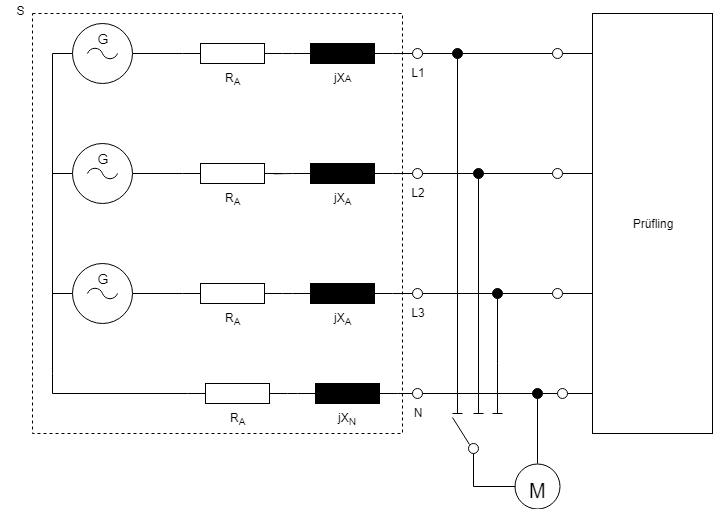
\includegraphics[scale=0.4]{Bezugsimpedanz.png}	
	\caption{Prüfspannungsquelle mit der Bezugsimpedanz}
	\label{fig:Bezugsimpedanz}
\end{figure}

\begin{table}[ht!]
	\begin{tabular}{ll}
		G  & Spannungsquelle                                                                                                                                                                                                                                               \\
		M  & Messeinrichtung                                                                                                                                                                                                                                               \\
		S  & \begin{tabular}[c]{@{}l@{}}Prüfungspannungsquelle, bestehend aus dem Spannungsgenerator  G und der\\ Bezugsimpedanz Z mit den Elemente\end{tabular}                                                                                                           \\
		& \begin{tabular}[c]{@{}l@{}}R$_A$ = $\SI{0.24}{\Omega}$  jX$_A$ = $\SI{0.15}{\Omega}$ bei $\SI{50}{Hz}$\\ R$_N$ = $\SI{0.16}{\Omega}$ jX$_A$ = $\SI{0.10}{\Omega}$ bei $\SI{50}{Hz}$\end{tabular}
	\end{tabular}
\end{table}

Die drei Quellenspannungen $G$ entsprechen der Nennspannung. Alle Spannungen werden auf die Nennspannung $Un$ normiert: Der Prüfkreis besteht aus der Prüfspannungsquelle, dem zu prüfenden Gerät (Prüfling) und einer Messeinrichtung, zum Beispiel Strommesser, Spannungszange oder einem Flickermeter (M).\\
Es gibt bei der Bezugsimpedanz keine Unterscheidung im Anwendungsbereich zwischen Haushaltsgeräten und gewerblich genutzten Geräten. Stattdessen wird die Langzeit-Flickerstärke eingeführt und auf 65 \% der Kurzzeit-Flickerstärke begrenzt \cite{FlickerNorm}.\\
Damit man versteht, welche Bedeutung der Flickerwert hat und wie er zustande gekommen ist, gibt es hier eine Kurze Erklärung des Begriffes:\\
Mithilfe des Flickerwertes kann man die Störempfindlichkeit des menschlichen Auges, auf Helligkeitsschwankungen bei der Beleuchtung, durch einen messbaren Wert ermitteln. Dieser Wert ist eine dimensionslose Zahl, welche das Störempfinden des Menschen ausdrückt, wenn er sich mit einer \SI{60}{W}-Glühbirne beleuchtet. Die Helligkeit variiert dabei auf Grund von Spannungsschwankungen. Erhält man den Wert 0, so bedeutet dies, dass praktisch keine Schwankungen der Spannungshöhe vorhanden und somit auch kein Flackern der Lampe ersichtlich ist.\\
Bei dem Wert 1 gibt es eine gewisse Helligkeitsschwankung, die als störend wahrgenommen wird. Jedoch sind die Resultate nicht aussagekräftig, da sie Orts-, Zeit- und Personen abhängig sind. Deshalb entwickelte man einen Algorithmus und ein entsprechendes Formelwerk für das Durchschnittsempfinden der Erkenntnisse. Mit Hilfe eines Flicker-Meters konnte ein geeignetes Messgerät entwickelt werden, welches mit einem Flickermessverfahren den Flickerwert berechnen konnte. Das Flicker-Meter liefert alle 10 Minuten einen Wert, der mit $Pst$ bezeichnet wird. Das $P$ steht dabei für $perceptibility units$ (Wahrnehmungseinheiten) und $st$ steht für $short time$. Der Wert, welcher man behandelt ist also der Kurzzeit-Flickerwert.\\
Die EN 50160-Norm sagt aus, dass man 12 aufeinander folgende $Pst$-Werte zusammenfassend zu einem $Plt$-Wert (long time-Flicker = Langzeit-Flicker) verrechnen kann. Genauer bedeutet dies, dass man die 12 $Pst$-Werte, die über 2 Stunden gemessen wurden, zusammenrechnet und daraus den Durchschnitt nimmt. Jeder einzelne $Pst$-Wert geht mit einer 3. Potenz in die Bewertung ein. Der $Plt$-Wert ist der kubische Mittelwert der 12 $Pst-Werte$ und ist in der unterstehenden Formel dargestellt \cite{Spannungsqualitaet}.

\begin{equation}\label{eq:Plt}
P_{lt} = {\sqrt[3]{\frac{\sum_{i=1}^{N} {P_{st,i}}^3}{N}}}
\end{equation}

Mithilfe dieser Norm können Typenprüfung für bestimmte Geräte vorgenommen werden. Das Ziel dieser Typenprüfung ist es, die Übereinstimmung mit den Grenzwerten festzustellen. Diese werden unter Laborbedingungen an einem Bezugsnetz betrieben. Bei den festgelegten Betriebsbedingungen werden die erzeugten Spannungsschwankungen in Bezug zu den Bezugsimpedanzen gemessen und beurteilt. Falls Geräte die Grenzwerte dieser Norm einhalten, kann davon ausgegangen werden, dass sie zu keinerlei Beschwerden im Netz Anlass geben. Die elektromagnetische Verträglichkeit ist daher gewährleistet \cite{FlickerNorm}. 


\subsubsection{EN 61000-2-2 Grenzwerte für Oberschwingungsspannungen}

Die folgende Norm beinhaltet die Festlegung für Verträglichkeitspegel von niederfrequenten, leitungsgeführten Störgrössen und für Signale von Netz-Kommunikationssystemen in öffentlichen Niederspannungs- und Stromversorgungsnetzen. Die Werte des Verträglichkeitspegels mit ihrer Eigenschaft können für die EMV-Koordinierung von Störaussendungs- und Störfestigkeitsanforderungen für Geräte und als Planungspegel für Stromversorgungsnetze verwendet werden. In der Norm werden folgende Phänomene betrachtet:

\begin{itemize}
	\item Spannungsschwankungen und Flicker 
	\item Oberschwingungen bis zur 50. Oberschwingungsordnung
	\item Zwischenharmonische
	\item Spannungsverzerrungen bei Frequenzen oberhalb der 50. Oberschwingungsordnung
	\item Spannungseinbrüche
	\item Kurzzeitunterbrechungen der Versorgungsspannung
	\item Spannungsunsymmetrien
	\item Kurzzeitunterbrechungen der Versorgungsspannung
	\item Transiente Überspannung
	\item Zweiteilige Schwankung der Netzfrequenz
\end{itemize}
Wobei man sagen kann, dass einige Punkt, wie zum Beispiel das Bestimmen des Flickerwertes oder die Langzeit- und die Kurzzeit Flickerstärke schon in der vorherigen Norm definiert sind.\\
Die Tabelle \ref{tab:kompatibilitätsstufen_ZF} zeigt die verschiedenen Kompatibilitätsstufen für einzelne Oberschwingungsspannungen im Niederspannungsnetz. Sie ist nur in Bezug auf Langzeiteffekte für einzelne harmonische Spannung definiert. Der Wert der gesamten harmonische Verzerrung darf hierbei höchstens einen Wert von $THD$ = 8\% betragen im stationären Betrieb.
\begin{table}[ht!]
	\centering
	\resizebox{\textwidth}{!}{%
		\begin{tabular}{|l|l|l|l|l|l|}
			\hline
			\multicolumn{2}{|c|}{\begin{tabular}[c]{@{}c@{}}Ungeradzahlige \\ Harmonische \\ nicht-vielfache von 3\end{tabular}}                                                            & \multicolumn{2}{c|}{\begin{tabular}[c]{@{}c@{}}Ungeradzahlige \\ Harmonische \\ Vielfache von 3\end{tabular}}                                                                     & \multicolumn{2}{c|}{\begin{tabular}[c]{@{}c@{}}Geradzahlige \\ Harmonische\end{tabular}}                                                                                          \\ \hline
			\multicolumn{1}{|c|}{\begin{tabular}[c]{@{}c@{}}Oberschwingungs\\ -ordnung\end{tabular}} & \multicolumn{1}{c|}{\begin{tabular}[c]{@{}c@{}}Harmonische \\ Spannung\end{tabular}} & \multicolumn{1}{c|}{\begin{tabular}[c]{@{}c@{}}Oberschwingungs\\ -ordnung\end{tabular}} & \multicolumn{1}{c|}{\begin{tabular}[c]{@{}c@{}}Harmonische \\ Spannung\end{tabular}} & \multicolumn{1}{c|}{\begin{tabular}[c]{@{}c@{}}Oberschwingungs\\ -ordnung\end{tabular}} & \multicolumn{1}{c|}{\begin{tabular}[c]{@{}c@{}}Harmonische \\ Spannung\end{tabular}} \\
			\multicolumn{1}{|c|}{\textit{h}}                                                                  & \multicolumn{1}{c|}{\%}                                                              & \multicolumn{1}{c|}{\textit{h}}                                                                     & \multicolumn{1}{c|}{\%}                                                              & \multicolumn{1}{c|}{\textit{h}}                                                                     & \multicolumn{1}{c|}{\%}                                                              \\ \hline
			
			5                                                         & 6                                                     & 3                                                       & 5                                                & 2                                           & 2                                         \\
			7                                                         & 5                                                     & 9                                                       & 1.5                                              & 4                                           & 1                                         \\
			11                                                        & 3.5                                                   & 15                                                      & 0.4                                              & 6                                           & 0.5                                       \\
			13                                                        & 3                                                     & 21                                                      & 0.3                                              & 8                                           & 0.5                                       \\
			17 $\leq$\textit{h}$\leq$ 49                                                   & 2.27x(17/\textit{h})-0.27                                   & 21<h$\leq$45                                                 & 0.2                                              & 10$\leq$\textit{h}$\leq$50                                     & 0.25x(10/\textit{h})+0.25                       \\ \hline
	\end{tabular}}
	\caption{Kompatibilitätsstufen für einzelne Oberschwingungsspannungen im Niederspannungsnetz}\label{tab:kompatibilitätsstufen_ZF}
\end{table}

Bei Kurzzeiteffekten wird ein Faktor k zu den harmonischen Ordnungen hinzu multipliziert. Dieser Faktor wird wie folgt berechnet: 
\begin{equation}\label{eq:factor_k_für_kurzzeiteffekte_ZF}
k = {1.3+\frac{0.7}{45}\cdot(h-5)}
\end{equation}
Der entsprechende Kompatibilitätsgrad für die gesamte harmonische Verzerrung liegt daher bei $THD$ = 11\%.



Die Tabelle \ref{tab:subharmonische_Spannung_ZF} zeigt die erforderlichen Werte in Prozent der subharmonischen Spannung im Niederspannungsnetz bei \SI{230}{V}, bei einer Frequenz von \SI{10}{Hz} bis \SI{90}{Hz}. Sie entsprechen dem Kompatibilitätsgrad bezüglich des Flimmerns.
\begin{table}[ht!]
	\centering
	\begin{tabular}{|l|l|l|}
		\hline
		\multicolumn{1}{|c|}{\multirow{3}{*}{\begin{tabular}[c]{@{}c@{}}Ordnung\\   {[}m{]}\end{tabular}}} & \multicolumn{2}{c|}{50 Hz System}                                                                                                                    \\ \cline{2-3} 
		\multicolumn{1}{|c|}{}                                                                             & \multicolumn{1}{c|}{\multirow{2}{*}{\begin{tabular}[c]{@{}c@{}}Subharmonische\\   Frequenzen fm {[}Hz{]}\end{tabular}}} & \multicolumn{1}{c|}{Um \%} \\ \cline{3-3} 
		\multicolumn{1}{|c|}{}                                                                             & \multicolumn{1}{c|}{}                                                                                                   & \multicolumn{1}{c|}{230V}  \\ \hline
		0.20 < m $\leq$ 0.60                                                                              & 10 < fm $\leq$ 30                                                                                                    & 0.51                        \\ \hline
		0.60 < m $\leq$ 0.64                                                                             & 30 < fm $\leq$ 32                                                                                                    & 0.43                        \\ \hline
		0.64 < m $\leq$ 0.68                                                                            & 32 < fm $\leq$ 34                                                                                                    & 0.35                        \\ \hline
		0.68 < m $\leq$ 0.72                                                                            & 34 < fm $\leq$ 36                                                                                                    & 0.28                        \\ \hline
		0.72 < m $\leq$ 0.76                                                                            & 36 < fm $\leq$ 38                                                                                                    & 0.23                        \\ \hline
		0.76 < m $\leq$ 0.84                                                                            & 38 < fm $\leq$ 42                                                                                                    & 0.18                        \\ \hline
		0.84 < m $\leq$ 0.88                                                                            & 42 < fm $\leq$ 44                                                                                                    & 0.18                        \\ \hline
		0.88 < m $\leq$ 0.92                                                                            & 44 < fm $\leq$ 46                                                                                                    & 0.24                        \\ \hline
		0.92 < m $\leq$ 0.96                                                                            & 46 < fm $\leq$ 48                                                                                                    & 0.36                        \\ \hline
		0.96 < m $\leq$ 1.04                                                                            & 48 < fm $\leq$ 52                                                                                                    & 0.64                        \\ \hline
		1.04 < m $\leq$ 1.08                                                                            & 52 < fm $\leq$ 54                                                                                                    & 0.36                        \\ \hline
		1.08 < m $\leq$ 1.12                                                                            & 54 < fm $\leq$ 56                                                                                                    & 0.24                        \\ \hline
		1.12 < m $\leq$ 1.16                                                                            & 56 < fm $\leq$ 58                                                                                                    & 0.18                        \\ \hline
		1.16 < m $\leq$ 1.24                                                                            & 58 < fm $\leq$ 62                                                                                                    & 0.18                        \\ \hline
		1.24 < m $\leq$ 1.28                                                                            & 62 < fm $\leq$ 64                                                                                                    & 0.23                        \\ \hline
		1.28 < m $\leq$ 1.32                                                                            & 64 < fm $\leq$ 66                                                                                                    & 0.28                        \\ \hline
		1.32 < m $\leq$ 1.36                                                                            & 66 < fm $\leq$ 68                                                                                                    & 0.35                        \\ \hline
		1.36 < m $\leq$ 1.40                                                                             & 68 < fm $\leq$ 70                                                                                                    & 0.43                        \\ \hline
		1.40 < m $\leq$ 1.80                                                                              & 70 < fm $\leq$ 90                                                                                                    & 0.51                        \\ \hline
	\end{tabular}
	\caption{Erforderlichen Werte der subharmonischen Spannungen}\label{tab:subharmonische_Spannung_ZF}
\end{table}

Einige Effekte, die wegen subharmonische Oberschwingung entstehen können sind:
\begin{itemize}
	\item Unerwünschter Strom, der in die Versorgungsnetze fliesst, welcher zusätzlicher Energieverlust verursacht.
	\item Subharmonische Spannungen stören den Betrieb von Leuchtstofflampen und anderen elektronischen Geräte, wie zum Beispiel Fernsehempfängern. Jede Verwendung von Strom und Spannungen, bei der die Höhe der Amplitude oder der Zeitpunkt des Nulldurchgangs wichtig ist, kann somit gestört werden, wenn die Kombination der vorhandenen unerwünschten Frequenz diese Eigenschaften der Versorgungsspannung ändern.
	\item Je grösser der Frequenzbereich ist und je grösser die Amplitude der Spannung bei diesen Frequenzen sind, desto grösser ist das Risiko unvorhersehbare Resonanzeffekte zu erhalten. Sie verstärkt die Spannungsverzerrung der Versorgungsspannung und führen zu einer Überlast oder anderen Störung bei den elektrischen Verbrauchern.
	\item Ein weiterer Effekt ist das Erzeugen von akustischen Geräuschen. Dies tritt jedoch vor allem bei einem Frequenzbereich von \SI{1}{kHz} bis \SI{9}{kHz} auf, bei der die Amplitude 0.5\% vom Frequenzwert abweicht und von der Art des beeinflussten Gerätes \cite{SpannungsNorm}.
\end{itemize}

\newpage
\section{Vergleich der Resultate von Plecs und Matlab}\label{sec:Vergleich_der_Resultate}

\begin{figure}[ht!]
	\centering
	\subfloat[][]{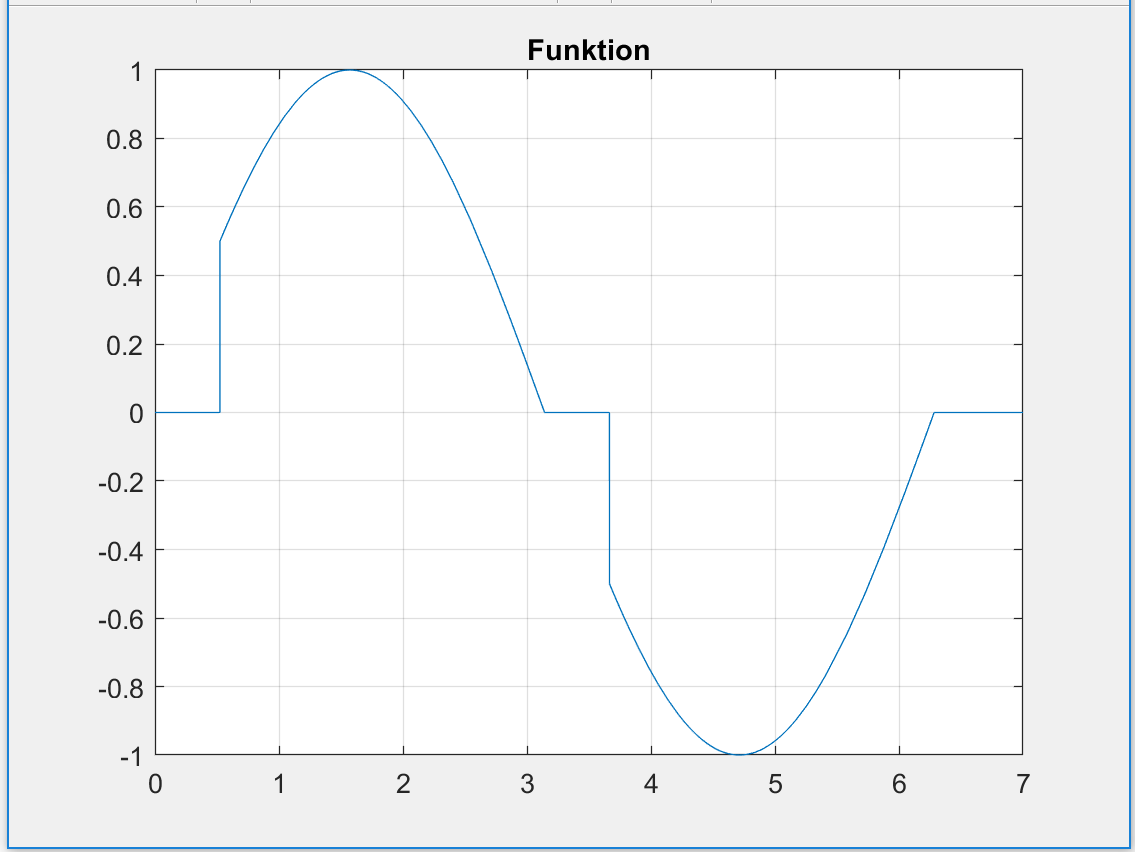
\includegraphics[width=0.4\linewidth]{eingangssignal_30.png}\label{fig:eingangssignal_30}}\qquad
	\subfloat[][]{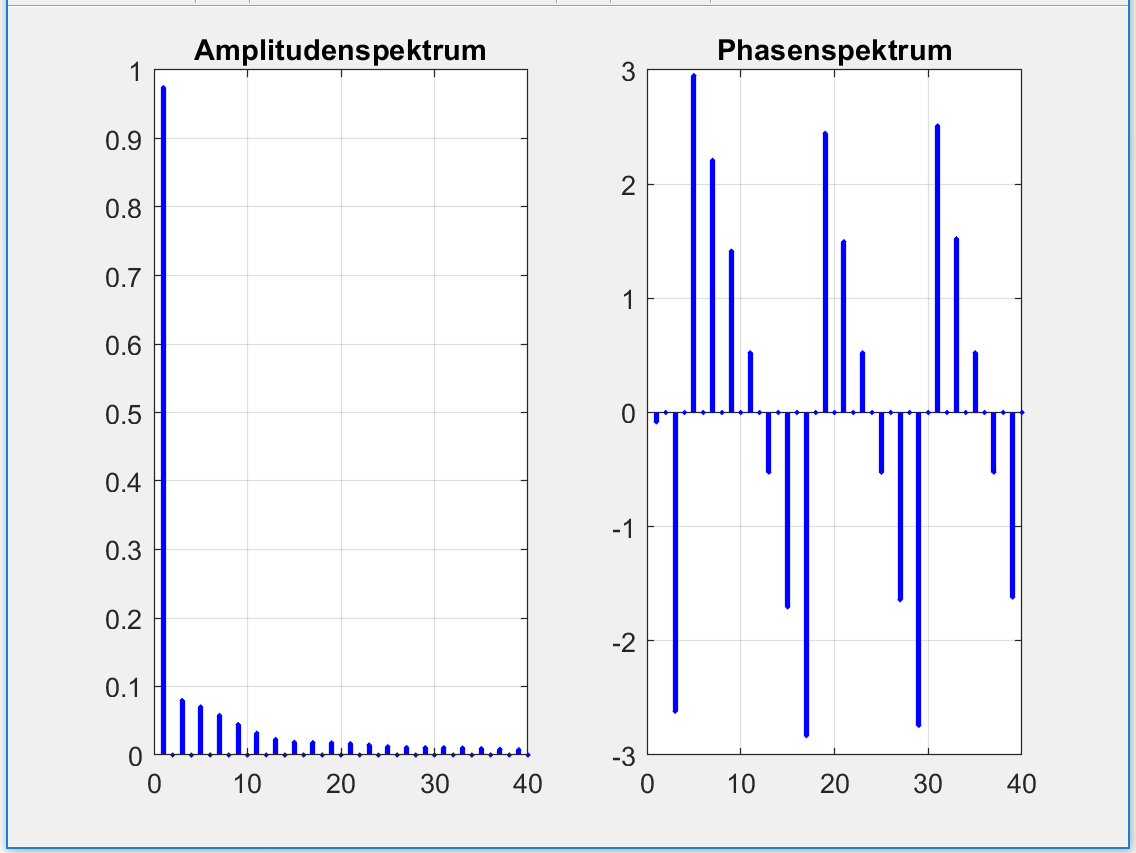
\includegraphics[width=0.4\linewidth]{A_PH_30.png}\label{fig:A_PH_30.}}
	\caption{Phasenanschnittsteuerung mit 30\textdegree (a) Eingangssignal (b) Amplituden- und Phasenspektrum}
	\label{fig:Phasenanschnittsteuerung_mit_30}
\end{figure}

\begin{figure}[ht!]
	\centering
	\subfloat[][]{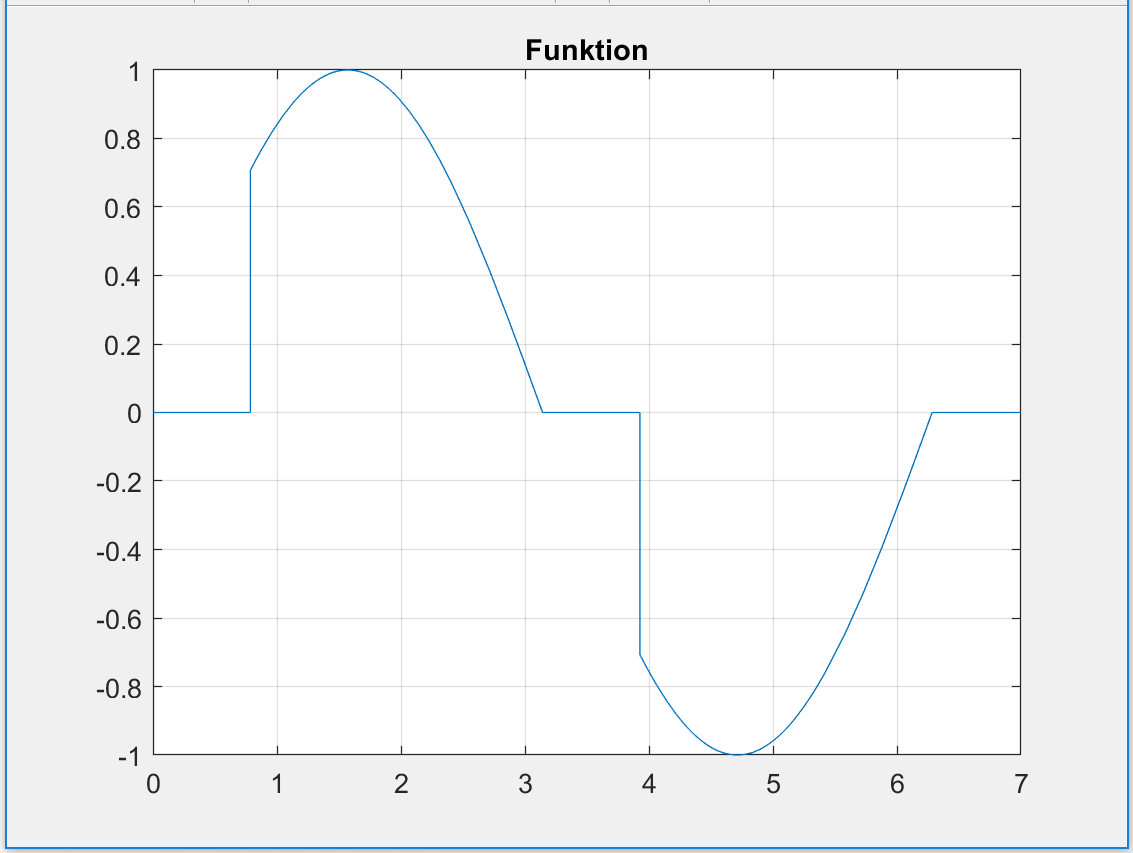
\includegraphics[width=0.4\linewidth]{eingangssignal_45.png}\label{fig:eingangssignal_45}}\qquad
	\subfloat[][]{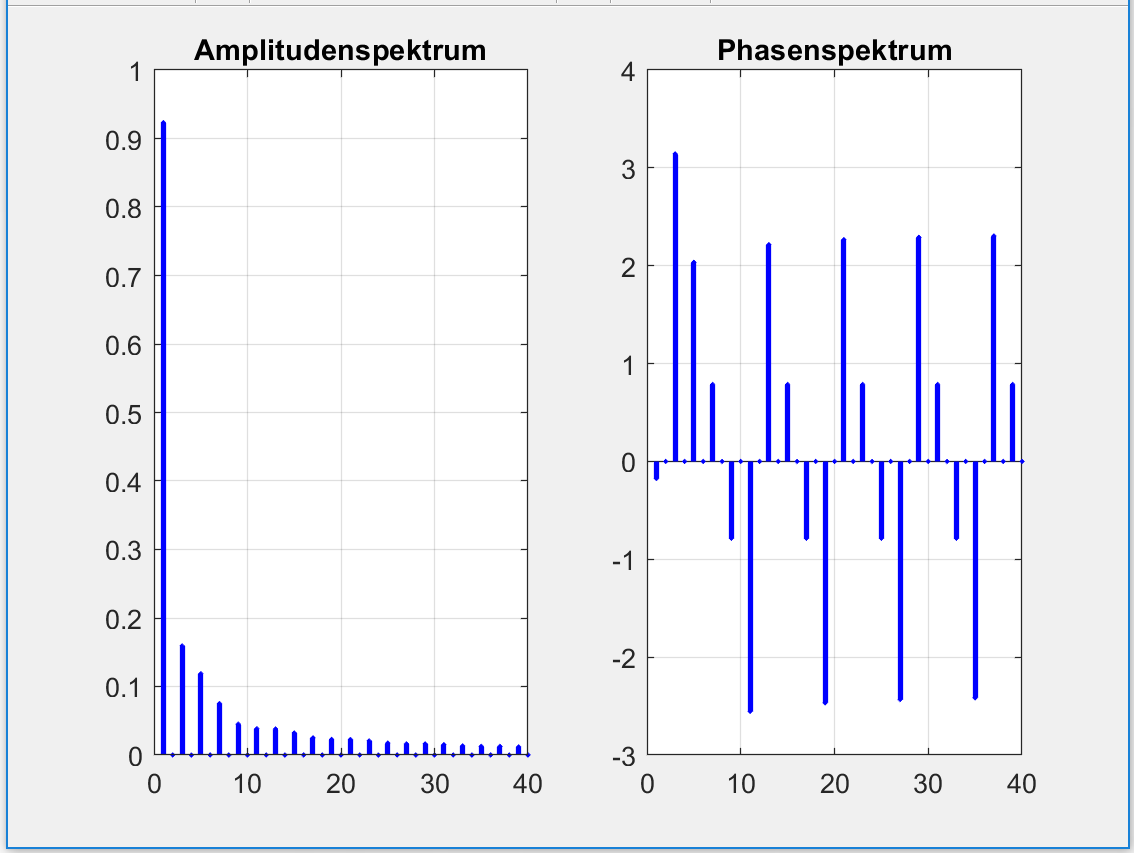
\includegraphics[width=0.4\linewidth]{A_PH_45.png}\label{fig:A_PH_45}}
	\caption{Phasenanschnittsteuerung mit 45\textdegree (a) Eingangssignal (b) Amplituden- und Phasenspektrum}
	\label{fig:Phasenanschnittsteuerung_mit_45}
\end{figure}

\begin{figure}[ht!]
	\centering
	\subfloat[][]{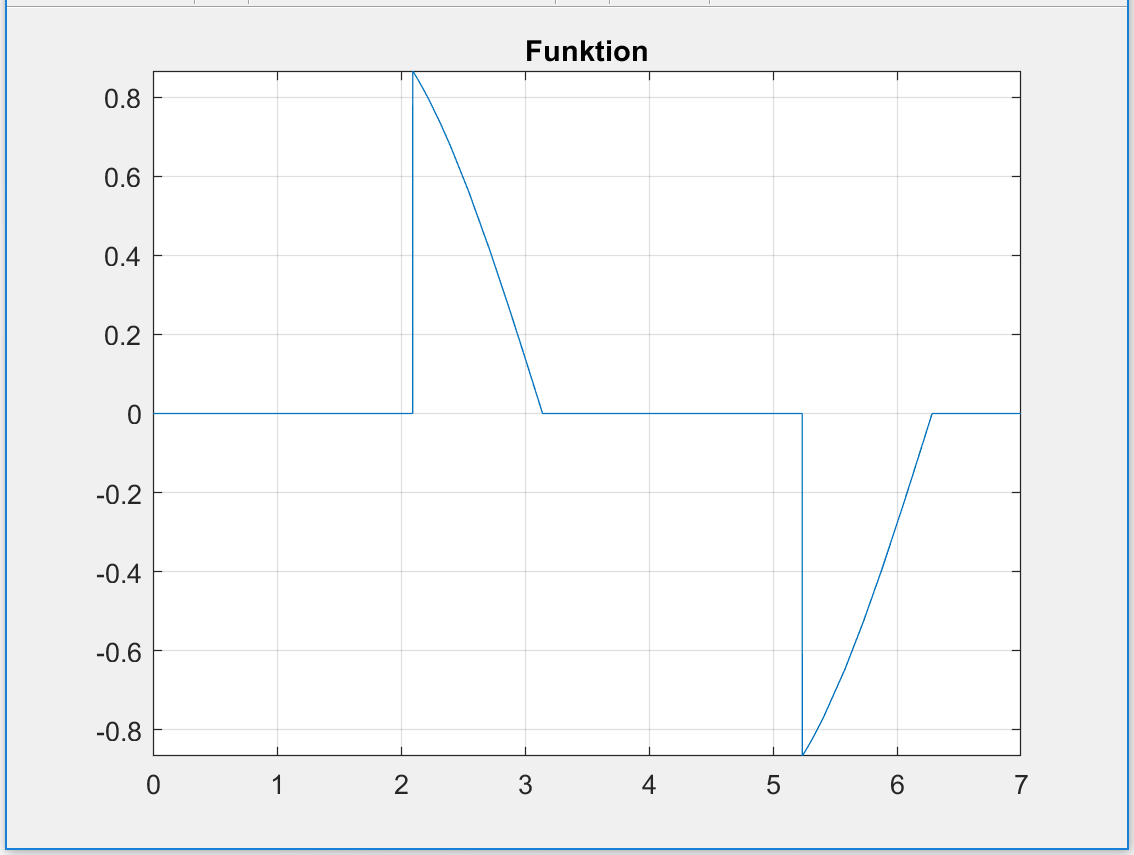
\includegraphics[width=0.4\linewidth]{eingangssignal_120.png}\label{fig:eingangssignal_120}}\qquad
	\subfloat[][]{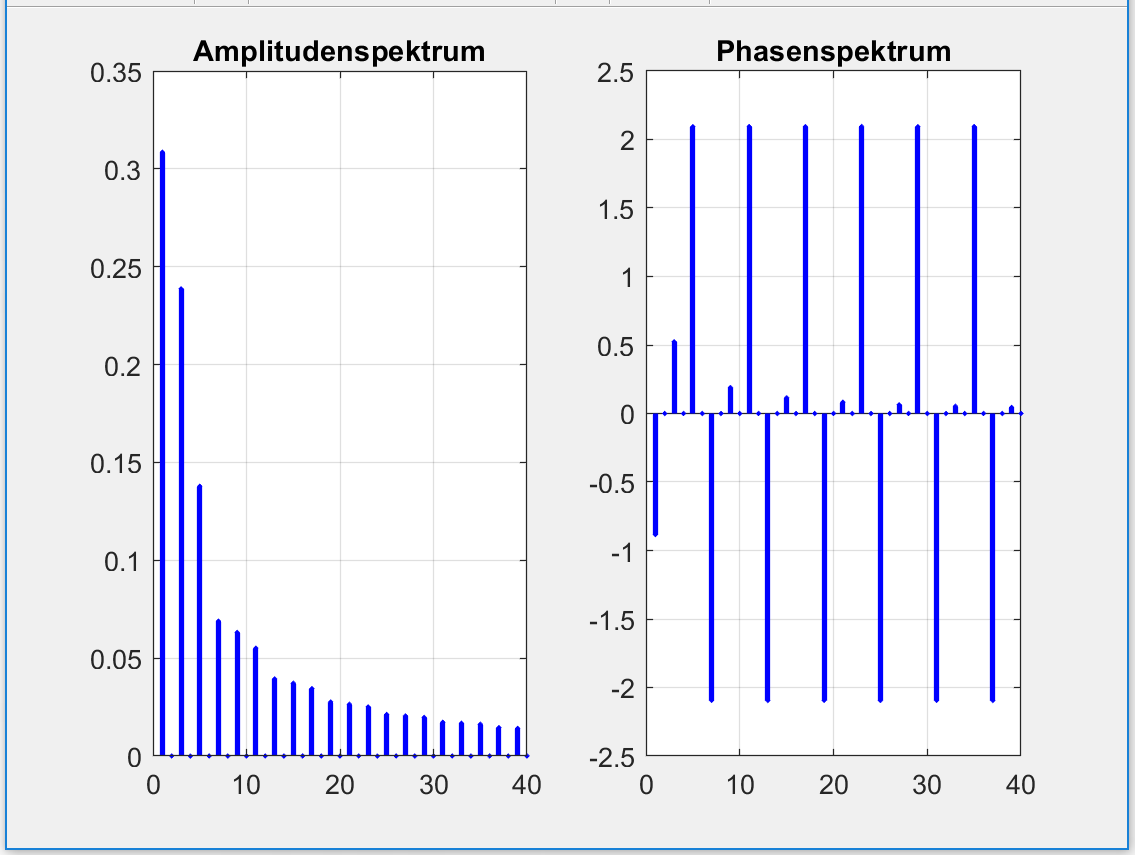
\includegraphics[width=0.4\linewidth]{A_PH_120.png}\label{fig:A_PH_120}}
	\caption{Phasenanschnittsteuerung mit 120\textdegree (a) Eingangssignal (b) Amplituden- und Phasenspektrum}
	\label{fig:Phasenanschnittsteuerung_mit_120}
\end{figure}

\newpage

\begin{figure}[ht!]
	\centering
	\subfloat[][]{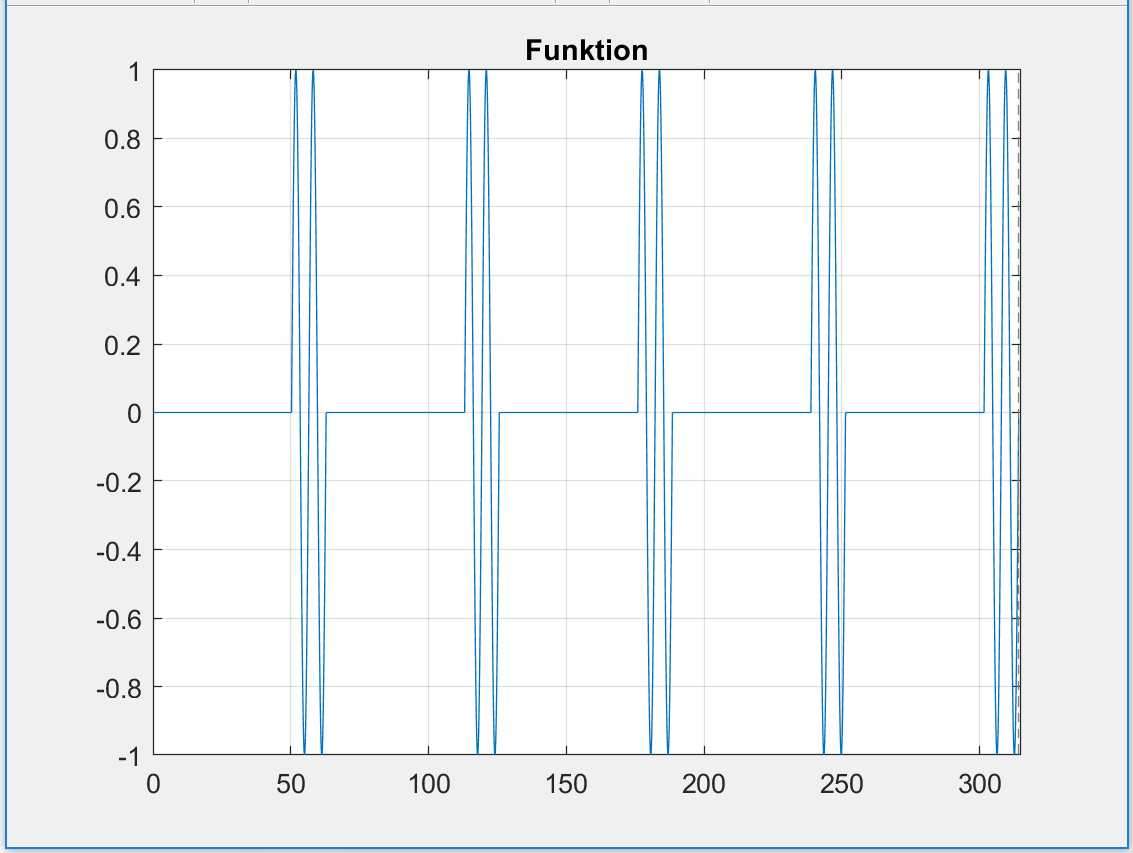
\includegraphics[width=0.4\linewidth]{Schwingungspaket_0_2.png}\label{fig:Schwingungspaket_0_2}}\qquad
	\subfloat[][]{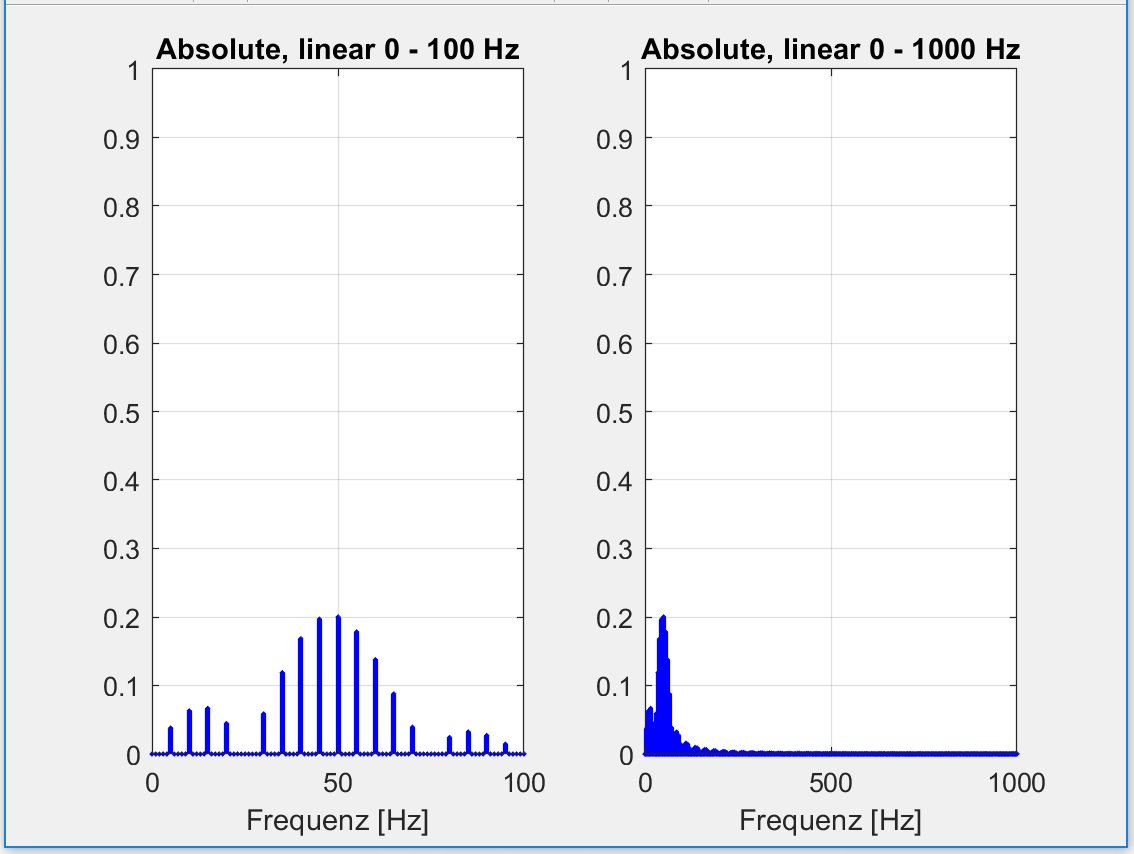
\includegraphics[width=0.4\linewidth]{Oberwellen_0_2.png}\label{fig:Oberwellen_0_2}}
	\caption{Schwingungspaket mit Duty Cycle 0.2 (a) Eingangssignal (b) Amplituden- und Phasenspektrum}
	\label{fig:Schwingungspaketsteuerung_mit_duty_cycle_0_2}
\end{figure}


\begin{figure}[ht!]
	\centering
	\subfloat[][]{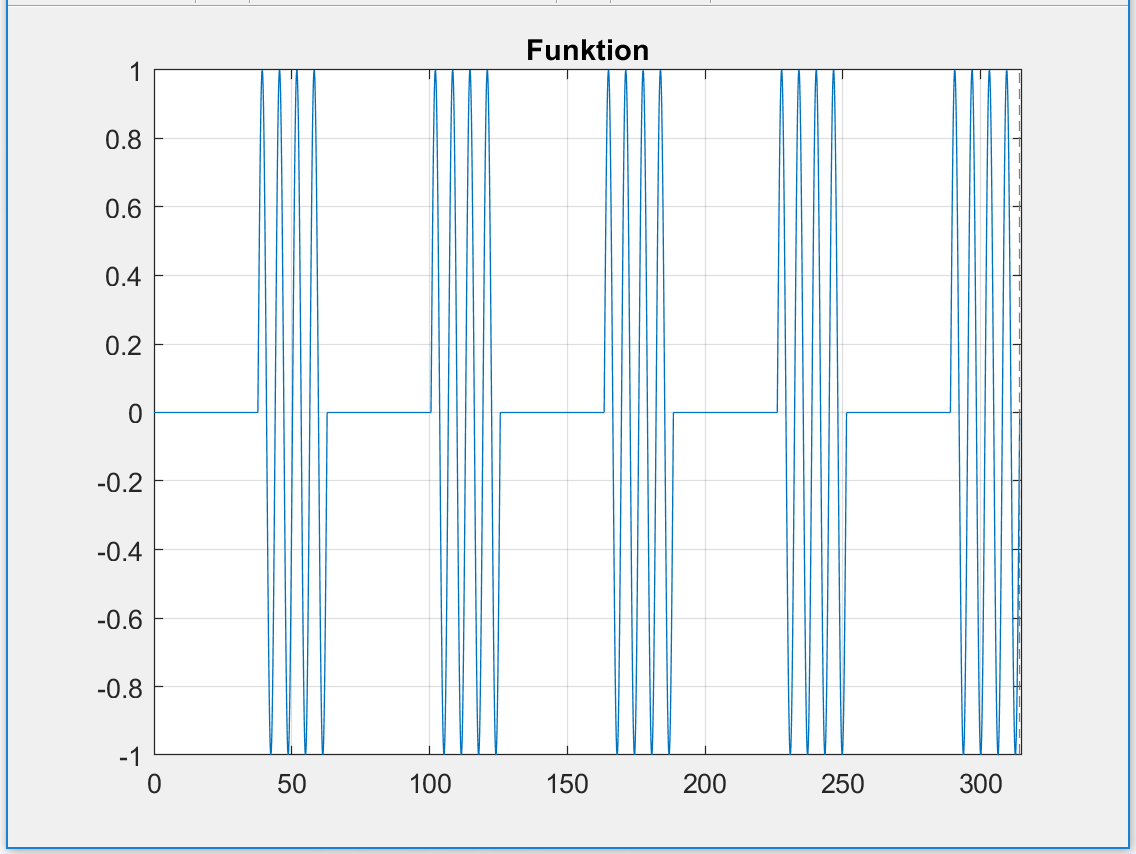
\includegraphics[width=0.4\linewidth]{Schwingungspaket_0_4.png}\label{fig:Schwingungspaket_0_4}}\qquad
	\subfloat[][]{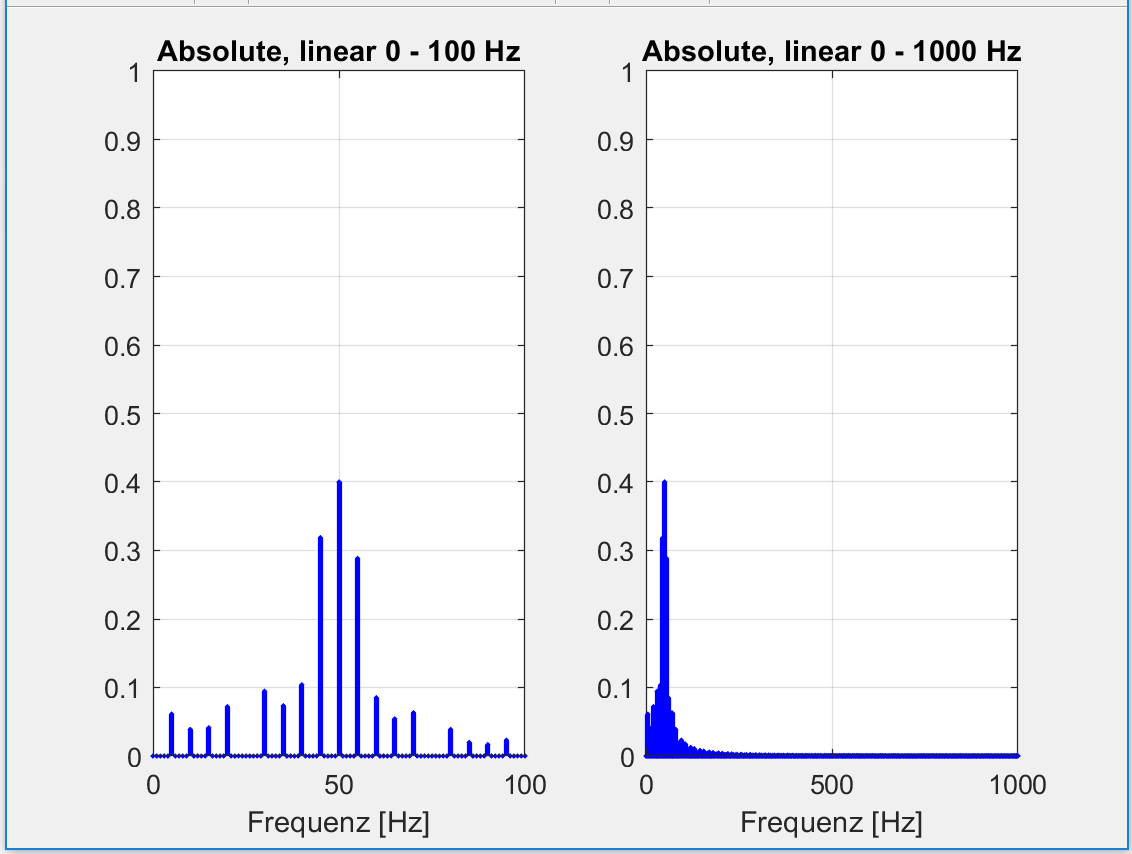
\includegraphics[width=0.4\linewidth]{Oberwellen_0_4.png}\label{fig:Oberwellen_0_4}}
	\caption{Schwingungspaket mit Duty Cycle 0.4 (a) Eingangssignal (b) Amplituden- und Phasenspektrum}
	\label{fig:Schwingungspaketsteuerung_mit_duty_cycle_0_4}
\end{figure}

\begin{figure}[ht!]
	\centering
	\subfloat[][]{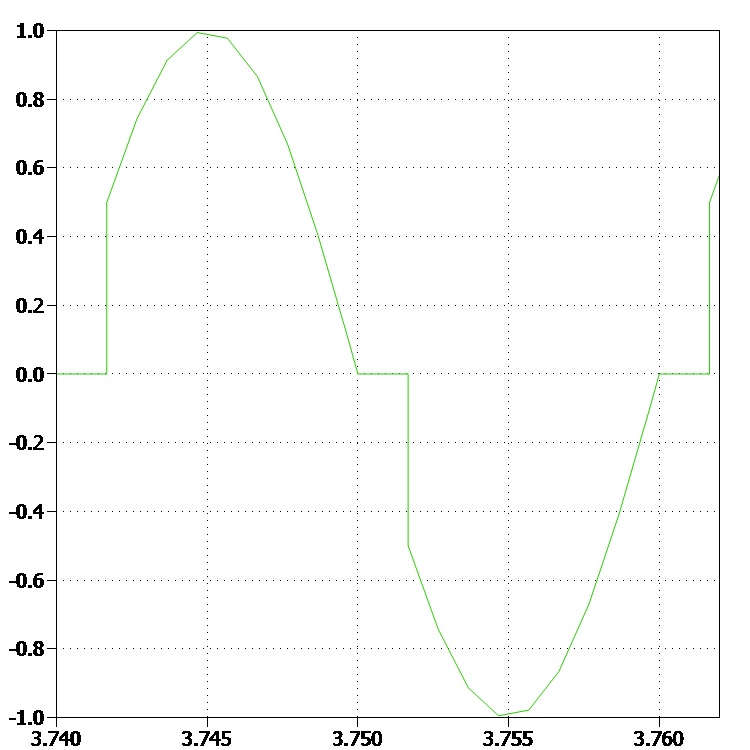
\includegraphics[width=0.32\linewidth]{plecs_phasenanschnitt_pi_6_funktion.png}\label{fig:plecs_phasenanschnitt_pi_6_funktion}}\qquad
	\subfloat[][]{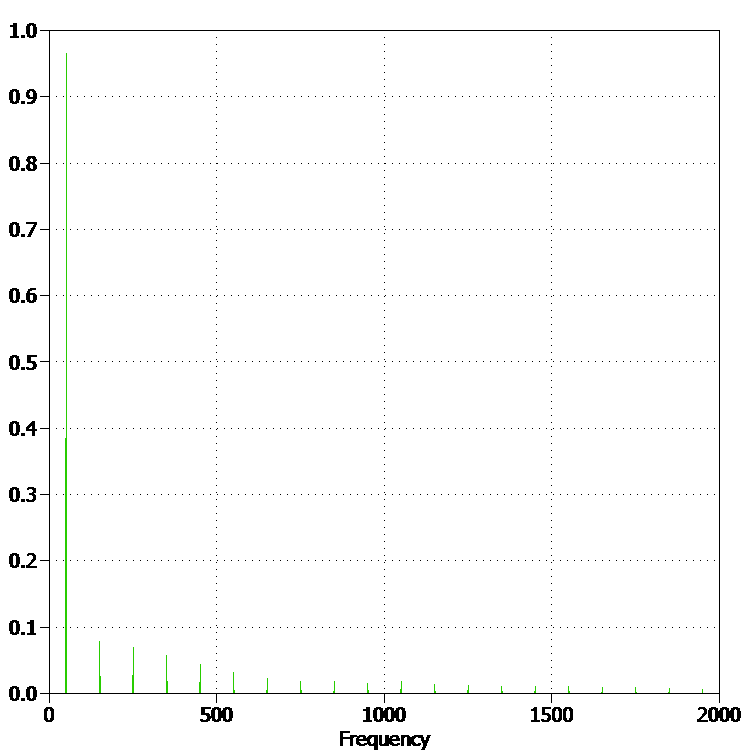
\includegraphics[width=0.32\linewidth]{plecs_phasenanschnitt_pi_6.png}\label{fig:plecs_phasenanschnitt_pi_6}}
	\caption{Phasenanschnitt mit 30\textdegree simuliert mit Plecs (a) Eingangssignal (b) Amplituden- und Phasenspektrum}
	\label{fig:Plecs_mit_phasenanschnitt_30}
\end{figure}

\newpage

\begin{figure}[ht!]
	\centering
	\subfloat[][]{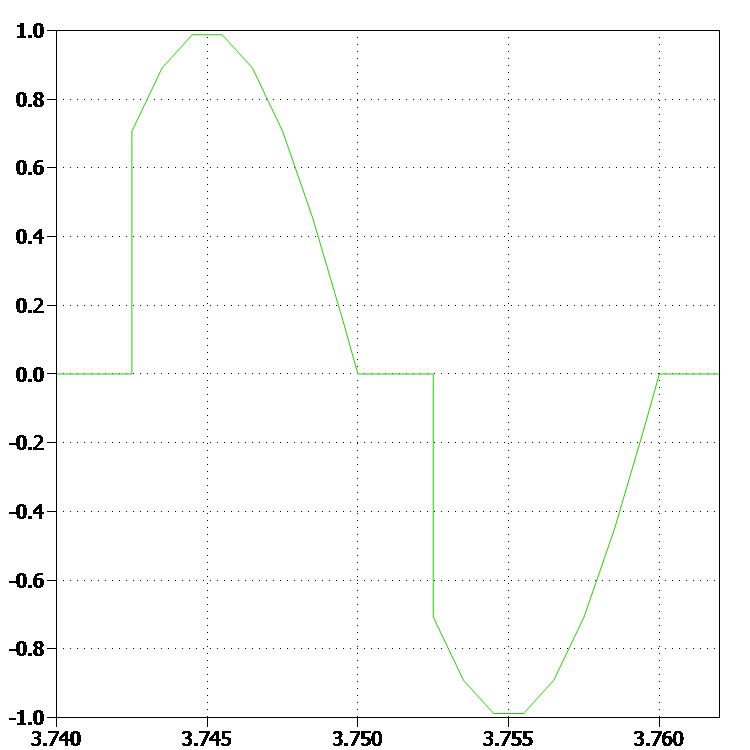
\includegraphics[width=0.32\linewidth]{plecs_phasenanschnitt_pi_4_funktion.png}\label{fig:plecs_phasenanschnitt_pi_4_funktion}}\qquad
	\subfloat[][]{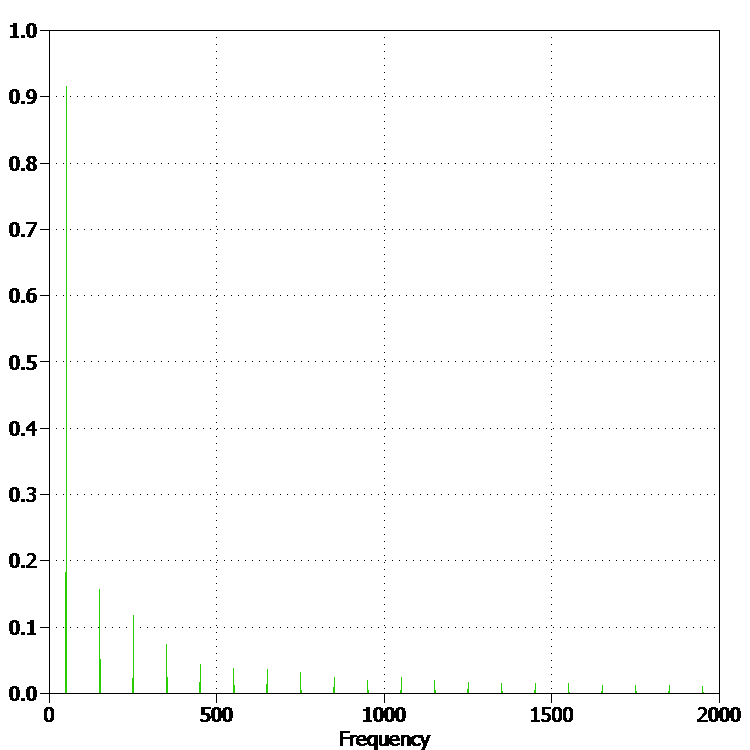
\includegraphics[width=0.32\linewidth]{plecs_phasenanschnitt_pi_4.png}\label{fig:plecs_phasenanschnitt_pi_4}}
	\caption{Phasenanschnitt mit 45\textdegree simuliert mit Plecs (a) Eingangssignal (b) Amplituden- und Phasenspektrum}
	\label{fig:Plecs_mit_phasenanschnitt_45}
\end{figure}


\begin{figure}[ht!]
	\centering
	\subfloat[][]{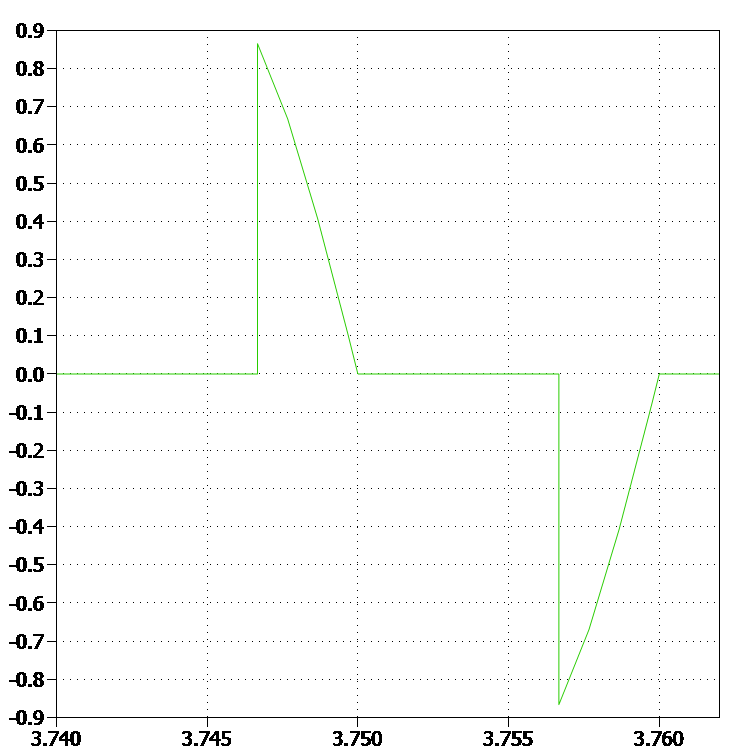
\includegraphics[width=0.32\linewidth]{plecs_phasenanschnitt_120_funktion.png}\label{fig:plecs_phasenanschnitt_120_funktion}}\qquad
	\subfloat[][]{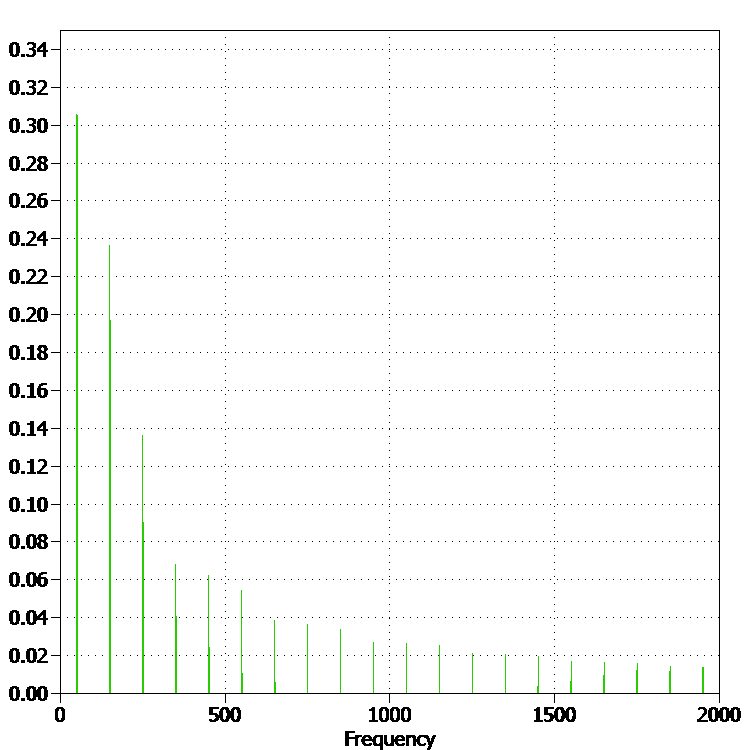
\includegraphics[width=0.32\linewidth]{plecs_phasenanschnitt_120.png}\label{fig:plecs_phasenanschnitt_120}}
	\caption{Phasenanschnitt mit 120\textdegree simuliert mit Plecs (a) Eingangssignal (b) Amplituden- und Phasenspektrum}
	\label{fig:Plecs_mit_phasenanschnitt_120}
\end{figure}


\begin{figure}[ht!]
	\centering
	\subfloat[][]{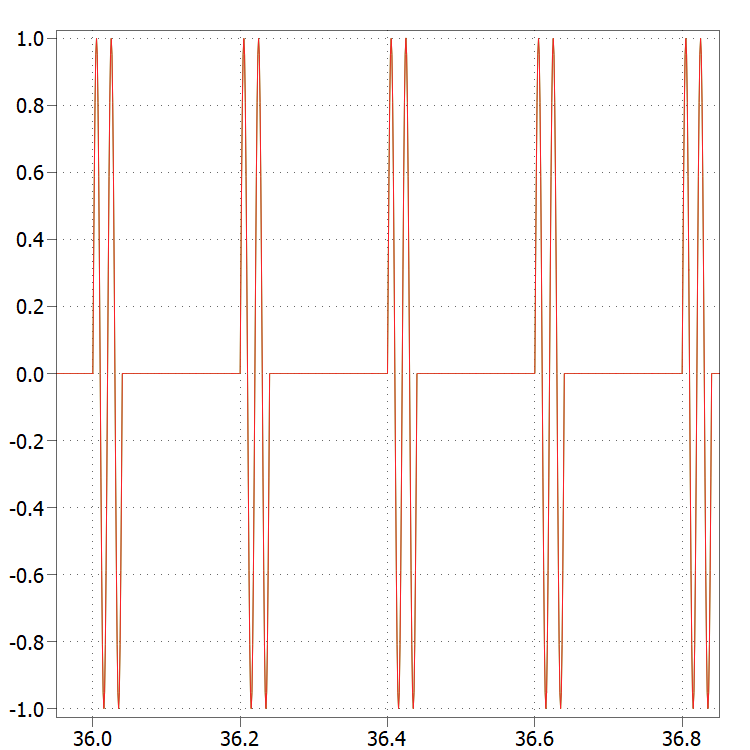
\includegraphics[width=0.32\linewidth]{plecs_schwingungspacket_0_2_schwingungen.PNG}\label{fig:plecs_schwingungspacket_0_2_schwingungen}}\qquad
	\subfloat[][]{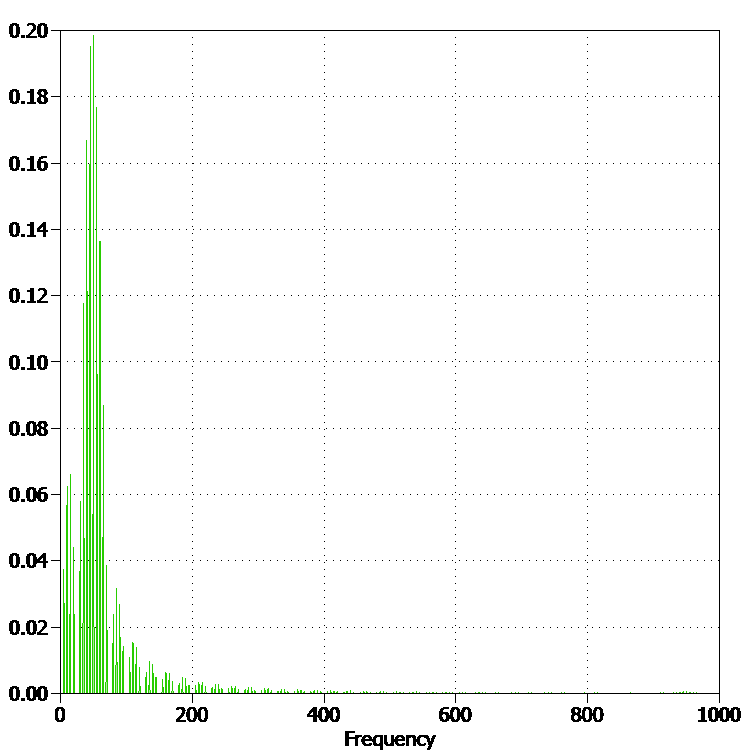
\includegraphics[width=0.32\linewidth]{plecs_schwingungspacket_0_2_1000.PNG}\label{fig:plecs_schwingungspacket_0_2_1000}}
	\caption{Schwingungspaketsteuerung mit Duty Cycle 0.2 simuliert mit Plecs (a) Eingangssignal (b) Amplitudenspektrum}
	\label{fig:Schwingungspaketsteuerung_mit_duty_cycle_0_2 simuliert_mit_Plecs}
\end{figure}

\newpage

\begin{figure}[ht!]
	\centering
	\subfloat[][]{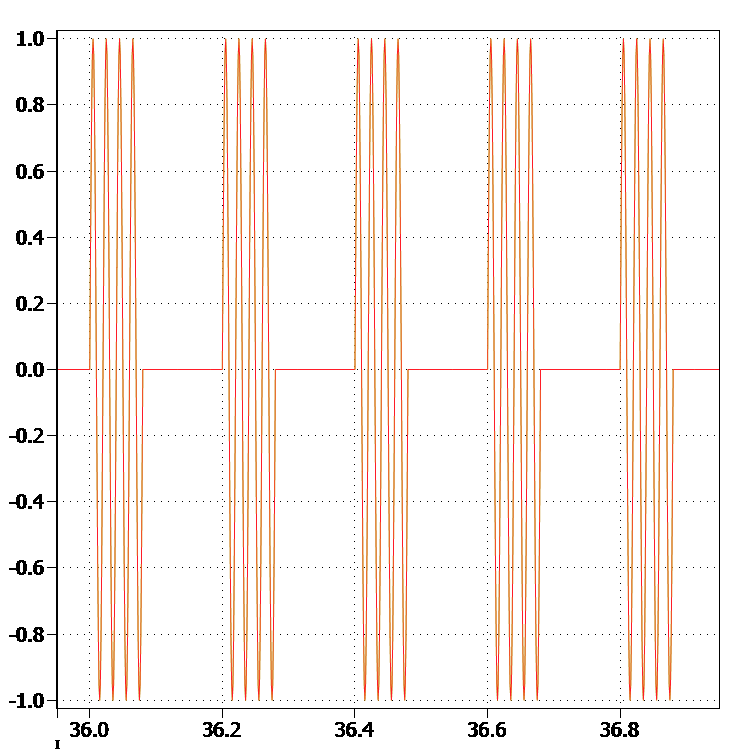
\includegraphics[width=0.32\linewidth]{plecs_schwingungspacket_0_4_schwingungen.PNG}\label{fig:plecs_schwingungspacket_0_4_schwingungen}}\qquad
	\subfloat[][]{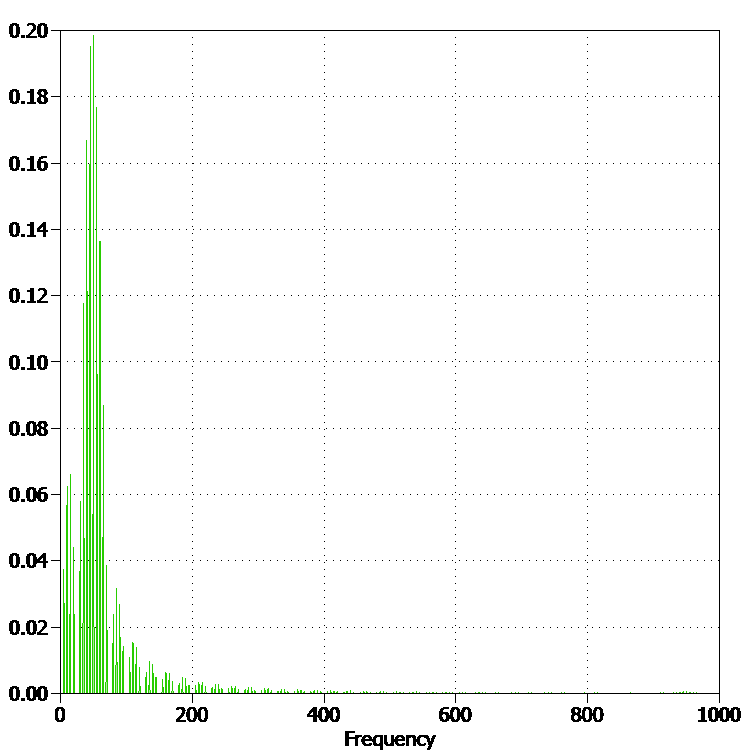
\includegraphics[width=0.32\linewidth]{plecs_schwingungspacket_0_2_1000.PNG}\label{fig:plecs_schwingungspacket_0_4_1000}}
	\caption{Schwingungspaketsteuerung mit Duty Cycle 0.4 simuliert mit Plecs (a) Eingangssignal (b) Amplitudenspektrum}
	\label{fig:Schwingungspaketsteuerung_mit_duty_cycle_0_4 simuliert_mit_Plecs}
\end{figure}

\begin{figure}[ht!]  
	\centering 
	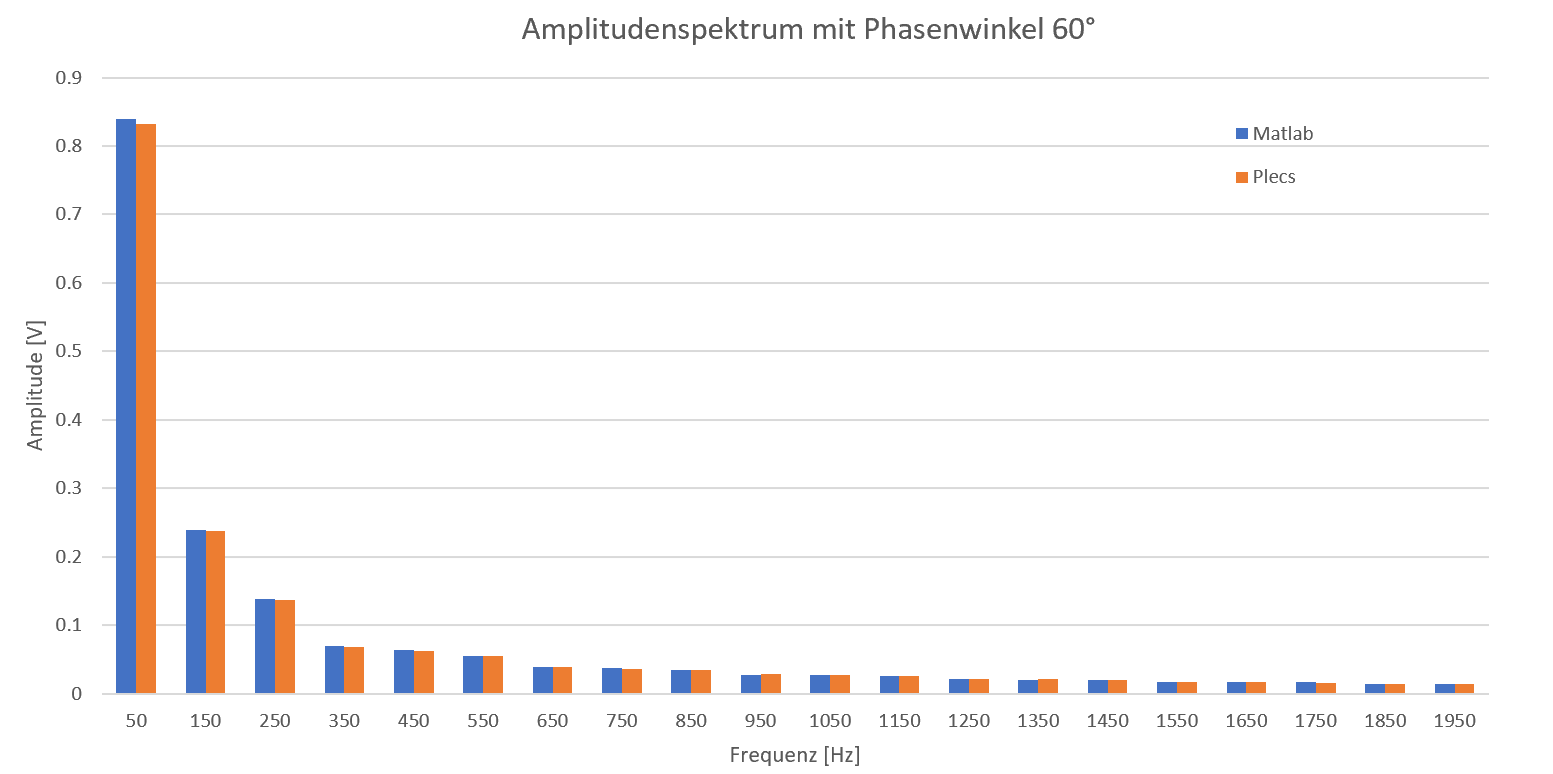
\includegraphics[scale=0.75]{Vergleich_Amplitudenspektrum_mit_Phasenwinkel_60.png}	
	\caption{Vergleich der Amplitudenspektrum mit Phasenwinkel von 60\textdegree}
	\label{fig:Vergleich_der_Amplitudenspektrum_mit Phasenwinkel_von_60}
\end{figure} 


\begin{figure}[ht!]
	\centering
	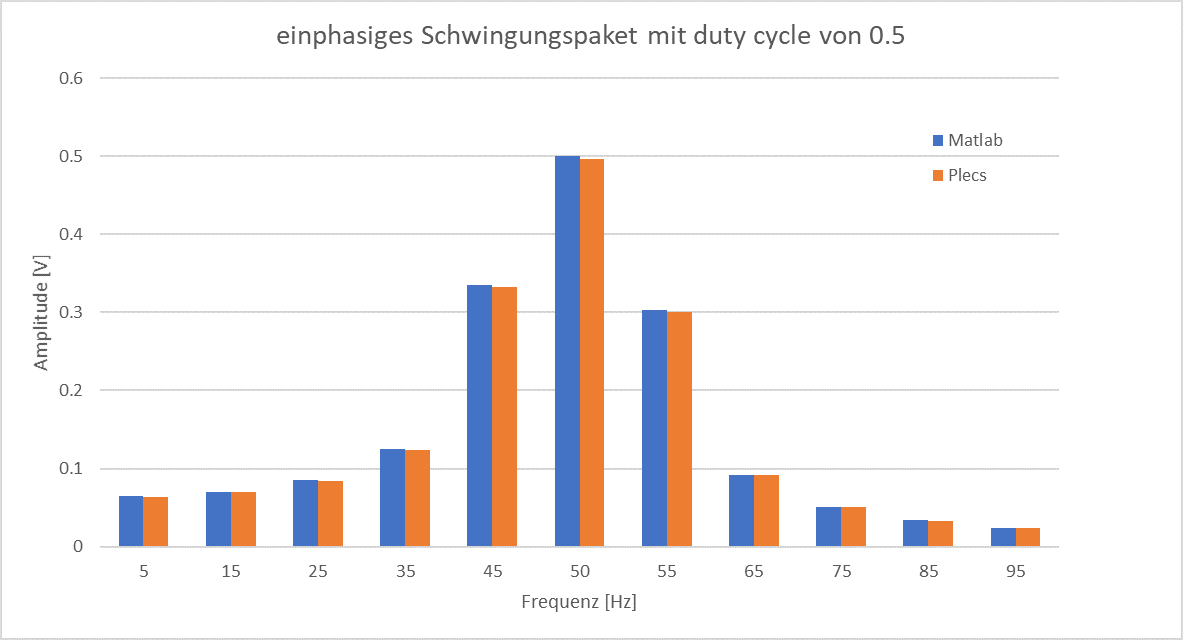
\includegraphics[scale=0.55]{Vergleich_einphasiges_Schwingungspaket_mit_duty_cycle_von_0_5.png}	
	\caption{Vergleich des Schwingungspaket mit Duty Cycle von 0.5}
	\label{fig:Vergleich des Schwingungspaket mit Duty Cycle von 0.5}
\end{figure}

\newpage

\begin{figure}[ht!]
	\centering
	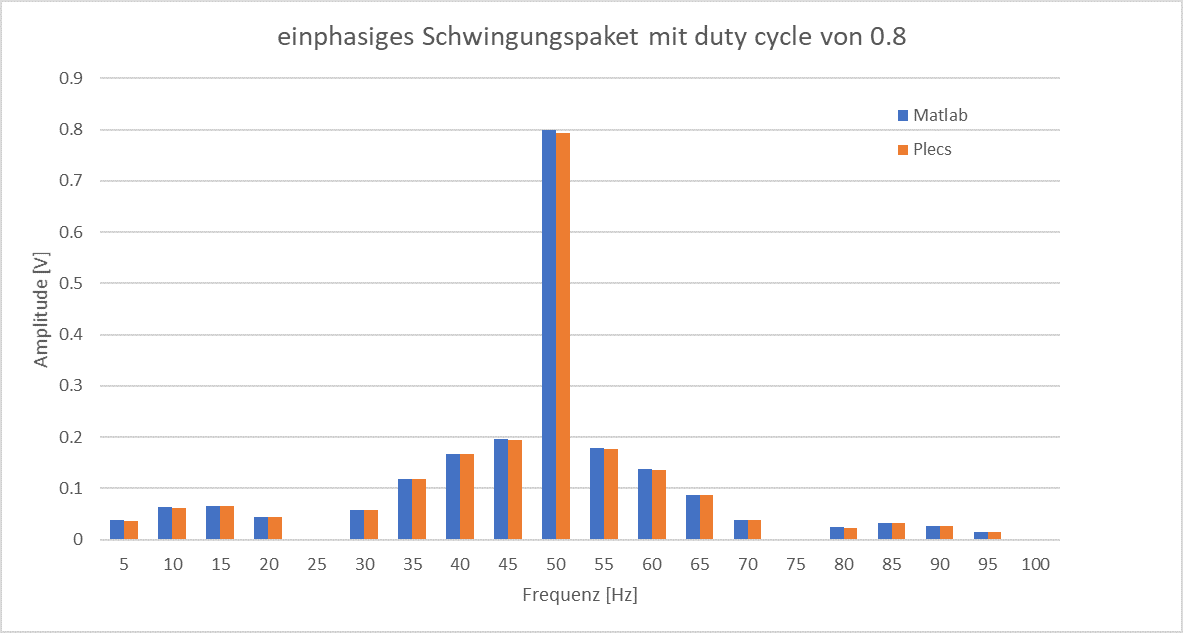
\includegraphics[scale=0.55]{Vergleich_einphasiges_Schwingungspaket_mit_duty_cycle_von_0_8.png}	
	\caption{Vergleich des Schwingungspaket mit Duty Cycle von 0.8}
	\label{fig:Vergleich des Schwingungspaket mit Duty Cycle von 0.8}
\end{figure}

\begin{figure}[ht!]
	\centering
	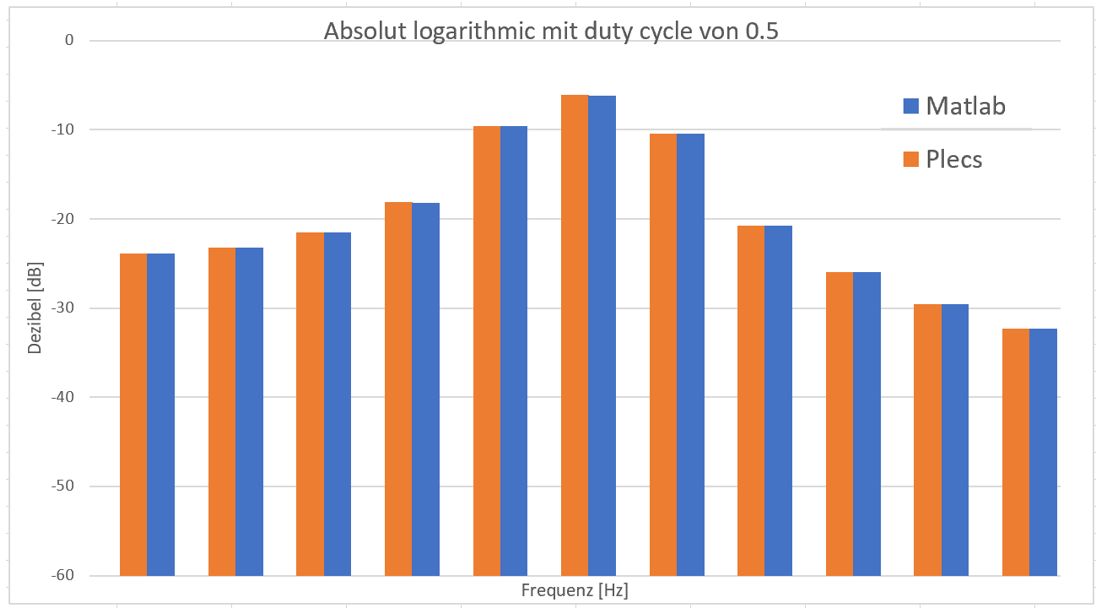
\includegraphics[scale=0.55]{Vergleich_absolut_logarithmic_duty_cycle_von_0_5_mit_legende.PNG}	
	\caption{Vergleich der absolut logarithmische Werte des Schwingungspaket mit Duty Cycle von 0.8}
	\label{fig:Vergleich_absolut_logarithmic_duty_cycle_von_0_5_mit_legende}
\end{figure}

\begin{figure}[ht!]
	\centering
	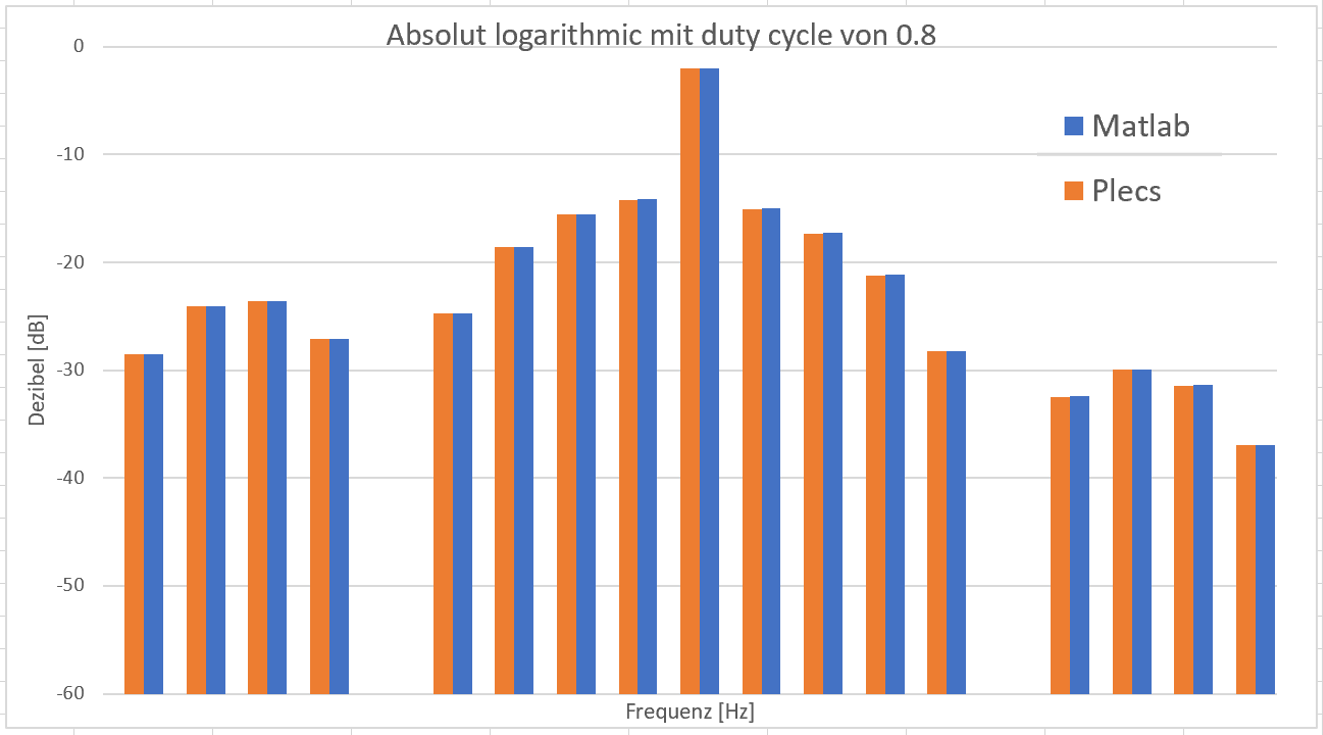
\includegraphics[scale=0.55]{Vergleich_absolut_logarithmic_duty_cycle_von_0_8_mit_legende.PNG}	
	\caption{Vergleich der absolut logarithmische Werte des Schwingungspaket mit Duty Cycle von 0.8}
	\label{fig:Vergleich_absolut_logarithmic_duty_cycle_von_0_8_mit_legende}
\end{figure}

\begin{minipage}{0.49\textwidth}
	\centering
	\begin{tabular}{|l|l|l|}
		\hline
		Frequenz & Matlab  & Plecs     \\ \hline
		50       & 0.8392  & 0.832293  \\ \hline
		150      & 0.2387  & 0.236735  \\ \hline
		250      & 0.1378  & 0.136638  \\ \hline
		350      & 0.06892 & 0.0683341 \\ \hline
		450      & 0.06316 & 0.0625278 \\ \hline
		550      & 0.05513 & 0.0545493 \\ \hline
		650      & 0.03938 & 0.0389562 \\ \hline
		750      & 0.03716 & 0.0365021 \\ \hline
		850      & 0.03446 & 0.0336658 \\ \hline
		950      & 0.02757 & 0.0278878 \\ \hline
		1050     & 0.0264  & 0.0276274 \\ \hline
		1150     & 0.02506 & 0.0253678 \\ \hline
		1250     & 0.0212  & 0.0213567 \\ \hline
		1350     & 0.02049 & 0.0205108 \\ \hline
		1450     & 0.01969 & 0.0196758 \\ \hline
		1550     & 0.01723 & 0.0172034 \\ \hline
		1650     & 0.01675 & 0.0166963 \\ \hline
		1750     & 0.01622 & 0.0161076 \\ \hline
		1850     & 0.01451 & 0.0143616 \\ \hline
		1950     & 0.01416 & 0.0137444 \\ \hline
	\end{tabular}
\captionof{table}{Vergleich der Werte des Phasenanschnittes mit 60\textdegree}
\label{tab:Phas_60_Vergleich}
\end{minipage}
%
\begin{minipage}{0.49\textwidth}
	\begin{tabular}{|l|l|l|}
		\hline
		Frequenz & Matlab  & Plecs     \\ \hline
		50       & 0.5927  & 0.587846  \\ \hline
		150      & 0.3183  & 0.3157    \\ \hline
		250      & 0.1061  & 0.105158  \\ \hline
		350      & 0.1061  & 0.105196  \\ \hline
		450      & 0.06366 & 0.0630047 \\ \hline
		550      & 0.06366 & 0.0630497 \\ \hline
		650      & 0.04547 & 0.044839  \\ \hline
		750      & 0.04547 & 0.0449042 \\ \hline
		850      & 0.03537 & 0.0342252 \\ \hline
		950      & 0.03537 & 0.0344228 \\ \hline
		1050     & 0.02894 & 0.0296088 \\ \hline
		1150     & 0.02894 & 0.0294399 \\ \hline
		1250     & 0.02449 & 0.0245782 \\ \hline
		1350     & 0.02449 & 0.0245363 \\ \hline
		1450     & 0.02122 & 0.0212078 \\ \hline
		1550     & 0.02122 & 0.0211877 \\ \hline
		1650     & 0.01872 & 0.0186503 \\ \hline
		1750     & 0.01872 & 0.0186415 \\ \hline
		1850     & 0.01675 & 0.0165256 \\ \hline
		1950     & 0.01675 & 0.0165378 \\ \hline
	\end{tabular}
\captionof{table}{Vergleich der Werte des Phasenanschnittes mit 90\textdegree}
\label{tab:Phas_90_Vergleich}
\end{minipage}

\newpage
\begin{minipage}{0.49\textwidth}
	\centering
	\begin{tabular}{|l|l|l|}
		\hline
		Frequenz & Matlab  & Plecs     \\ \hline
		5        & 0.06431 & 0.0637753 \\ \hline
		15       & 0.06996 & 0.0693821 \\ \hline
		25       & 0.08488 & 0.0841842 \\ \hline
		35       & 0.1248  & 0.123802  \\ \hline
		45       & 0.3351  & 0.332314  \\ \hline
		50       & 0.5     & 0.495901  \\ \hline
		55       & 0.3032  & 0.30067   \\ \hline
		65       & 0.09226 & 0.09151   \\ \hline
		75       & 0.05093 & 0.0505147 \\ \hline
		85       & 0.03368 & 0.0334101 \\ \hline
		95       & 0.02439 & 0.0241942 \\ \hline
	\end{tabular}
	\captionof{table}{Vergleich der Werte des Schwingungspaketes mit einem Duty Cycle von 0.5}
	\label{tab:Schwing_50_Vergleich}
\end{minipage}
%
\begin{minipage}{0.49\textwidth}
	\begin{tabular}{|l|l|l|}
		\hline
		Frequenz & Matlab & Plecs    \\ \hline
		5        & -23.84 & -23.907  \\ \hline
		15       & -23.1  & -23.175  \\ \hline
		25       & -21.42 & -21.4954 \\ \hline
		35       & -18.07 & -18.1455 \\ \hline
		45       & -9.497 & -9.56903 \\ \hline
		50       & -6.021 & -6.0921  \\ \hline
		55       & -10.37 & -10.4382 \\ \hline
		65       & -20.7  & -20.7706 \\ \hline
		75       & -25.86 & -25.9316 \\ \hline
		85       & -29.45 & -29.5225 \\ \hline
		95       & -32.26 & -32.3258 \\ \hline
	\end{tabular}
	\captionof{table}{Vergleich der absolut logarithmische Werte des Schwingungspaketes mit einem Duty Cycle von 0.5}
	\label{tab:abs_Schwing_50_Vergleich} 	
\end{minipage}

\begin{minipage}{0.49\textwidth}
	\centering
	\begin{tabular}{|l|l|l|}
		\hline
		Frequenz & Matlab & Plecs    \\ \hline
		5        & -28.45 & -28.5226 \\ \hline
		10       & -24    & -24.0755 \\ \hline
		15       & -23.54 & -23.6109 \\ \hline
		20       & -27.02 & -27.0954 \\ \hline
		25       &        &          \\ \hline
		30       & -24.66 & -24.7333 \\ \hline
		35       & -18.51 & -18.5814 \\ \hline
		40       & -15.48 & -15.5559 \\ \hline
		45       & -14.11 & -14.1847 \\ \hline
		50       & -1.938 & -2.0097  \\ \hline
		55       & -14.98 & -15.0538 \\ \hline
		60       & -17.23 & -17.2987 \\ \hline
		65       & -21.14 & -21.2065 \\ \hline
		70       & -28.18 & -28.2546 \\ \hline
		75       &        &          \\ \hline
		80       & -32.4  & -32.4725 \\ \hline
		85       & -29.89 & -29.9583 \\ \hline
		90       & -31.36 & -31.4339 \\ \hline
		95       & -36.87 & -36.9414 \\ \hline
	\end{tabular}
	\captionof{table}{Vergleich der absolut logarithmische Werte des Schwingungspaketes mit einem Duty Cycle von 0.8}
	\label{tab:abs_Schwing_80_Vergleich}
\end{minipage}
%
\begin{minipage}{0.49\textwidth}
	\begin{tabular}{|l|l|l|}
		\hline
		Frequenz & Matlab  & Plecs     \\ \hline
		5        & 0.0378  & 0.0374862 \\ \hline
		10       & 0.06307 & 0.0625494 \\ \hline
		15       & 0.06653 & 0.0659863 \\ \hline
		20       & 0.04455 & 0.0441804 \\ \hline
		25       & 0       & 0         \\ \hline
		30       & 0.05847 & 0.0579873 \\ \hline
		35       & 0.1187  & 0.117742  \\ \hline
		40       & 0.1682  & 0.166803  \\ \hline
		45       & 0.1969  & 0.195329  \\ \hline
		50       & 0.8     & 0.793442  \\ \hline
		55       & 0.1782  & 0.176729  \\ \hline
		60       & 0.1376  & 0.136479  \\ \hline
		65       & 0.08775 & 0.0870312 \\ \hline
		70       & 0.03898 & 0.0386607 \\ \hline
		75       & 0       & 0         \\ \hline
		80       & 0.02399 & 0.0237918 \\ \hline
		85       & 0.03203 & 0.0317749 \\ \hline
		90       & 0.02703 & 0.0268104 \\ \hline
		95       & 0.01434 & 0.014221  \\ \hline
		100      & 0       & 0         \\ \hline
	\end{tabular}
\captionof{table}{Vergleich der Werte des des Schwingungspaketes mit einem Duty Cycle von 0.8}
\label{tab:Schwing_80_Vergleich}
\end{minipage}


\newpage
\section{Messungen}
\subsection{Messungen Spannungen Widerstand}\label{sec:Mess_Spannung_Widerstand}
\subsubsection*{Phasenanschnitt 60\textdegree}

\begin{figure}[ht!]
	\centering
	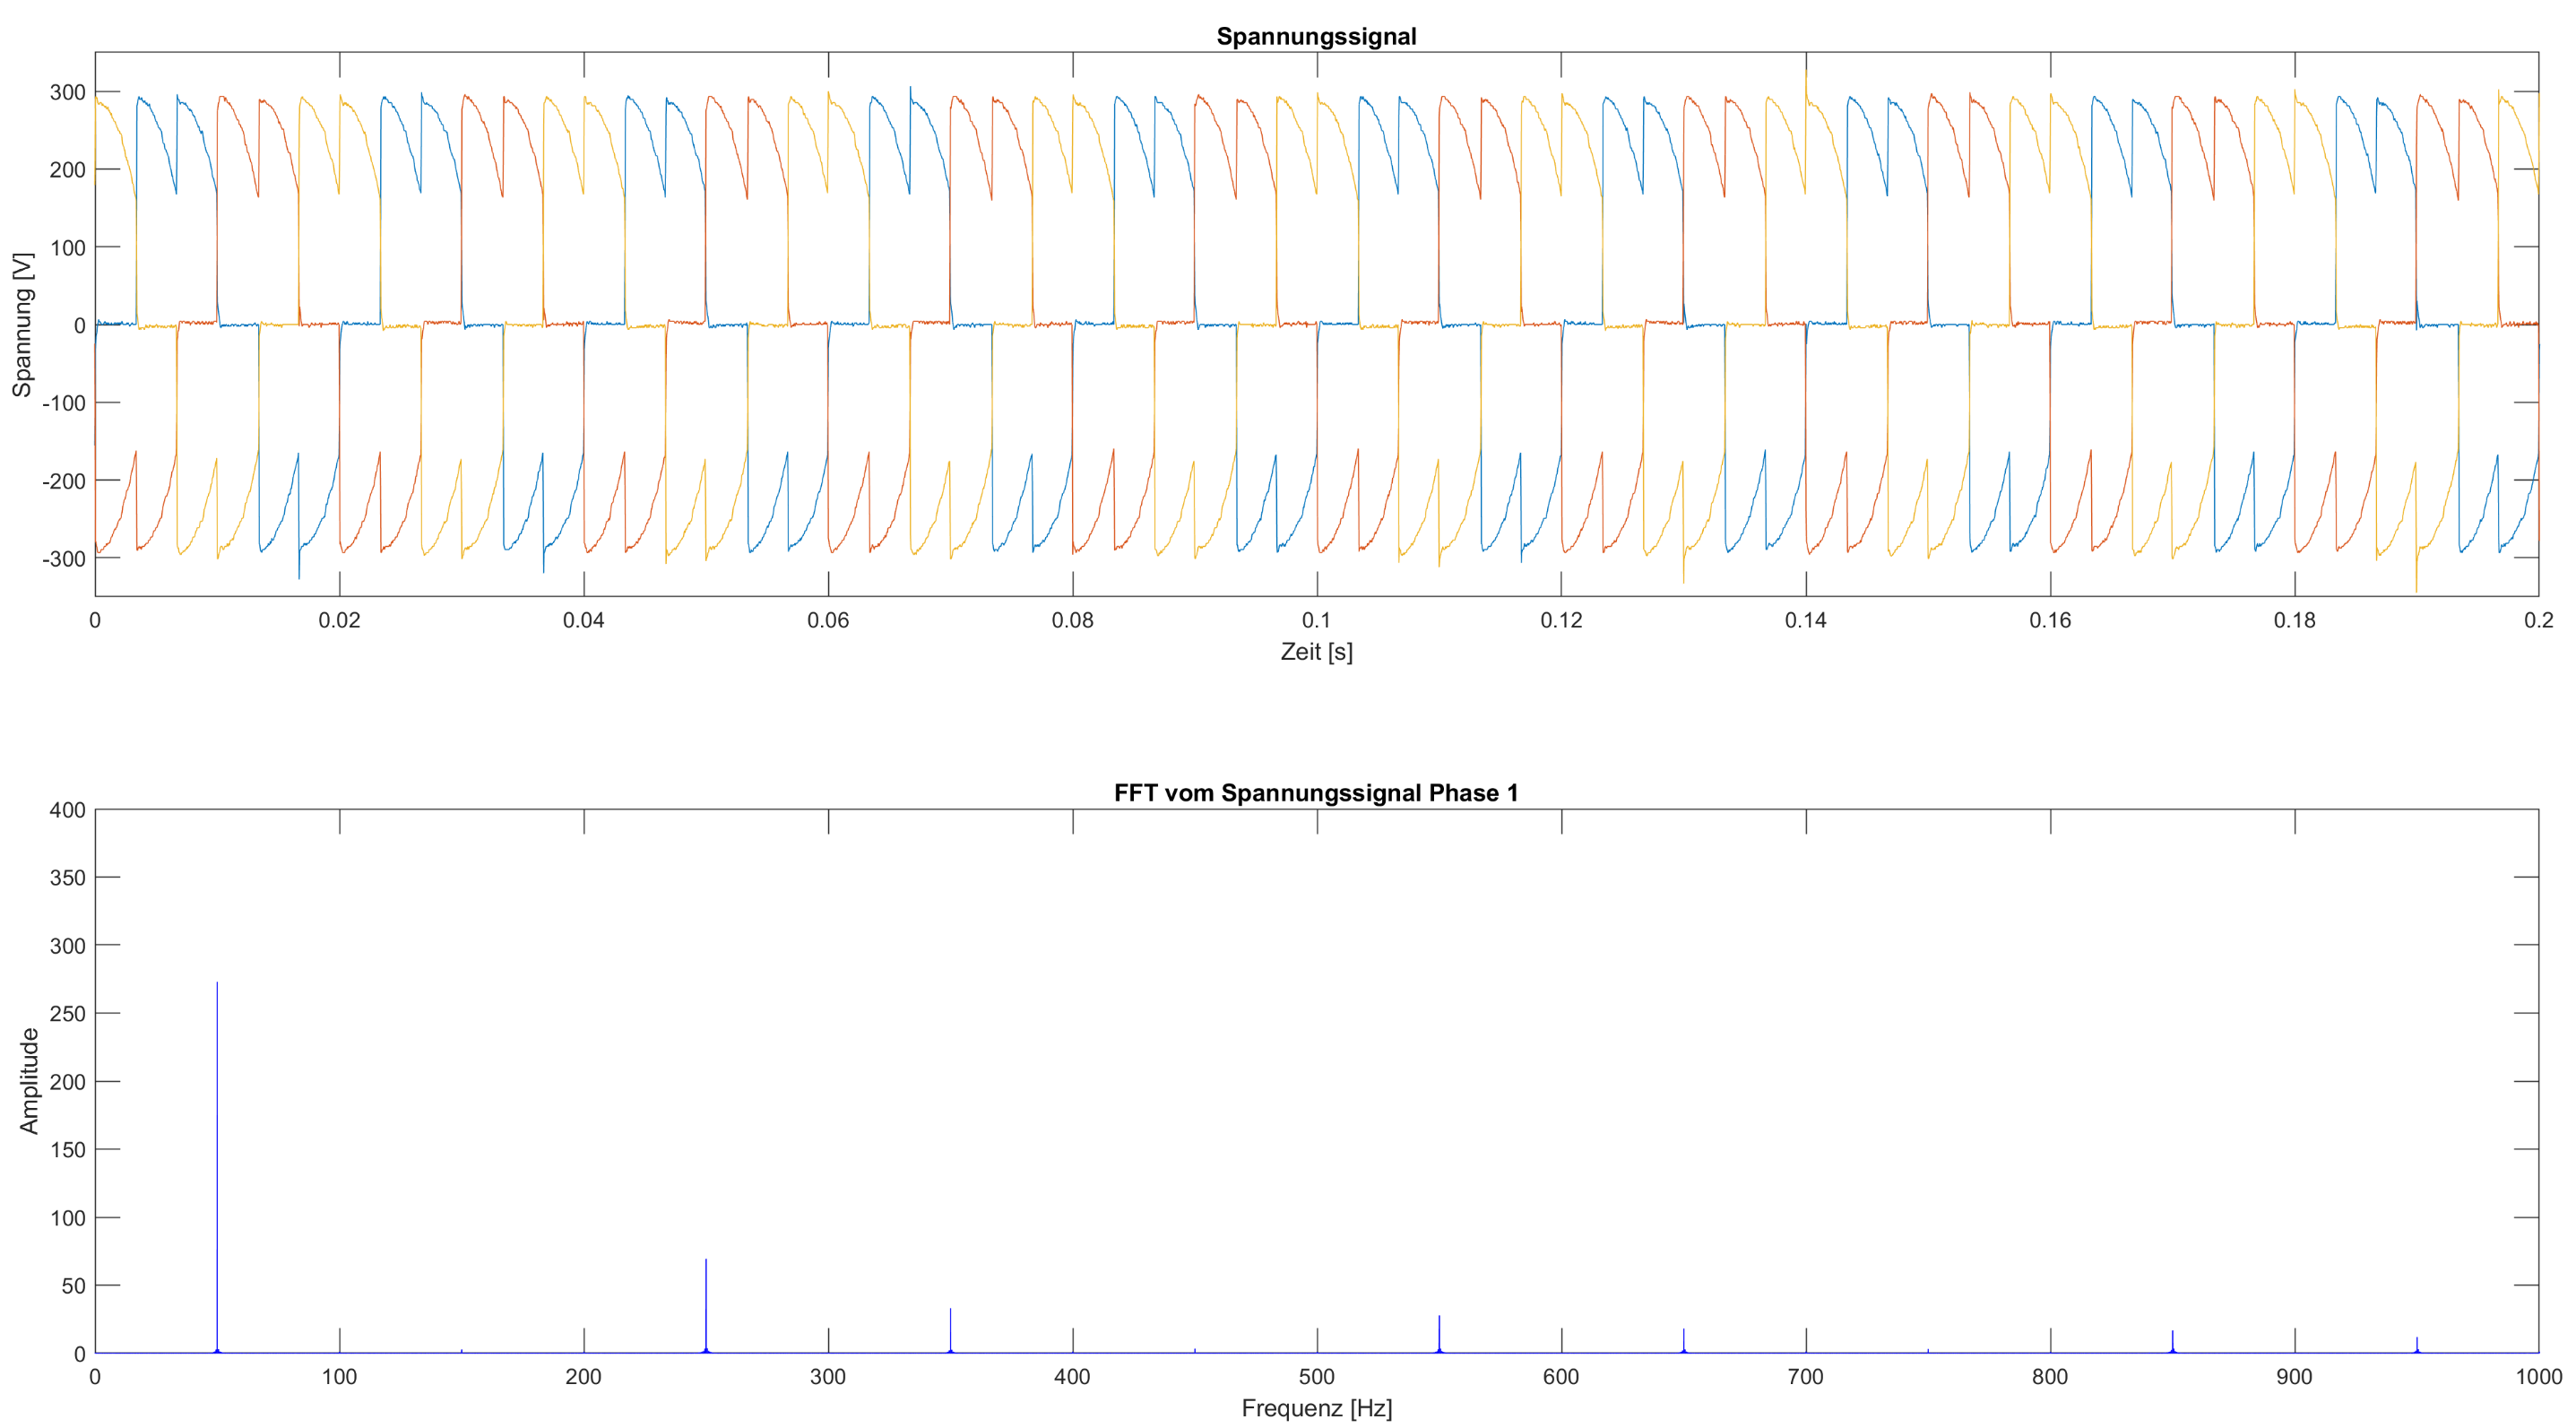
\includegraphics[width=0.96\textwidth]{Messung_Widerstand_Phas_60grad.png}	
	\caption{Messung mit Phasenanschnitt 60\textdegree}\label{fig:Mess_Phas_60}
\end{figure}

\subsubsection*{Phasenanschnitt 90\textdegree}
\begin{figure}[ht!]
	\centering
	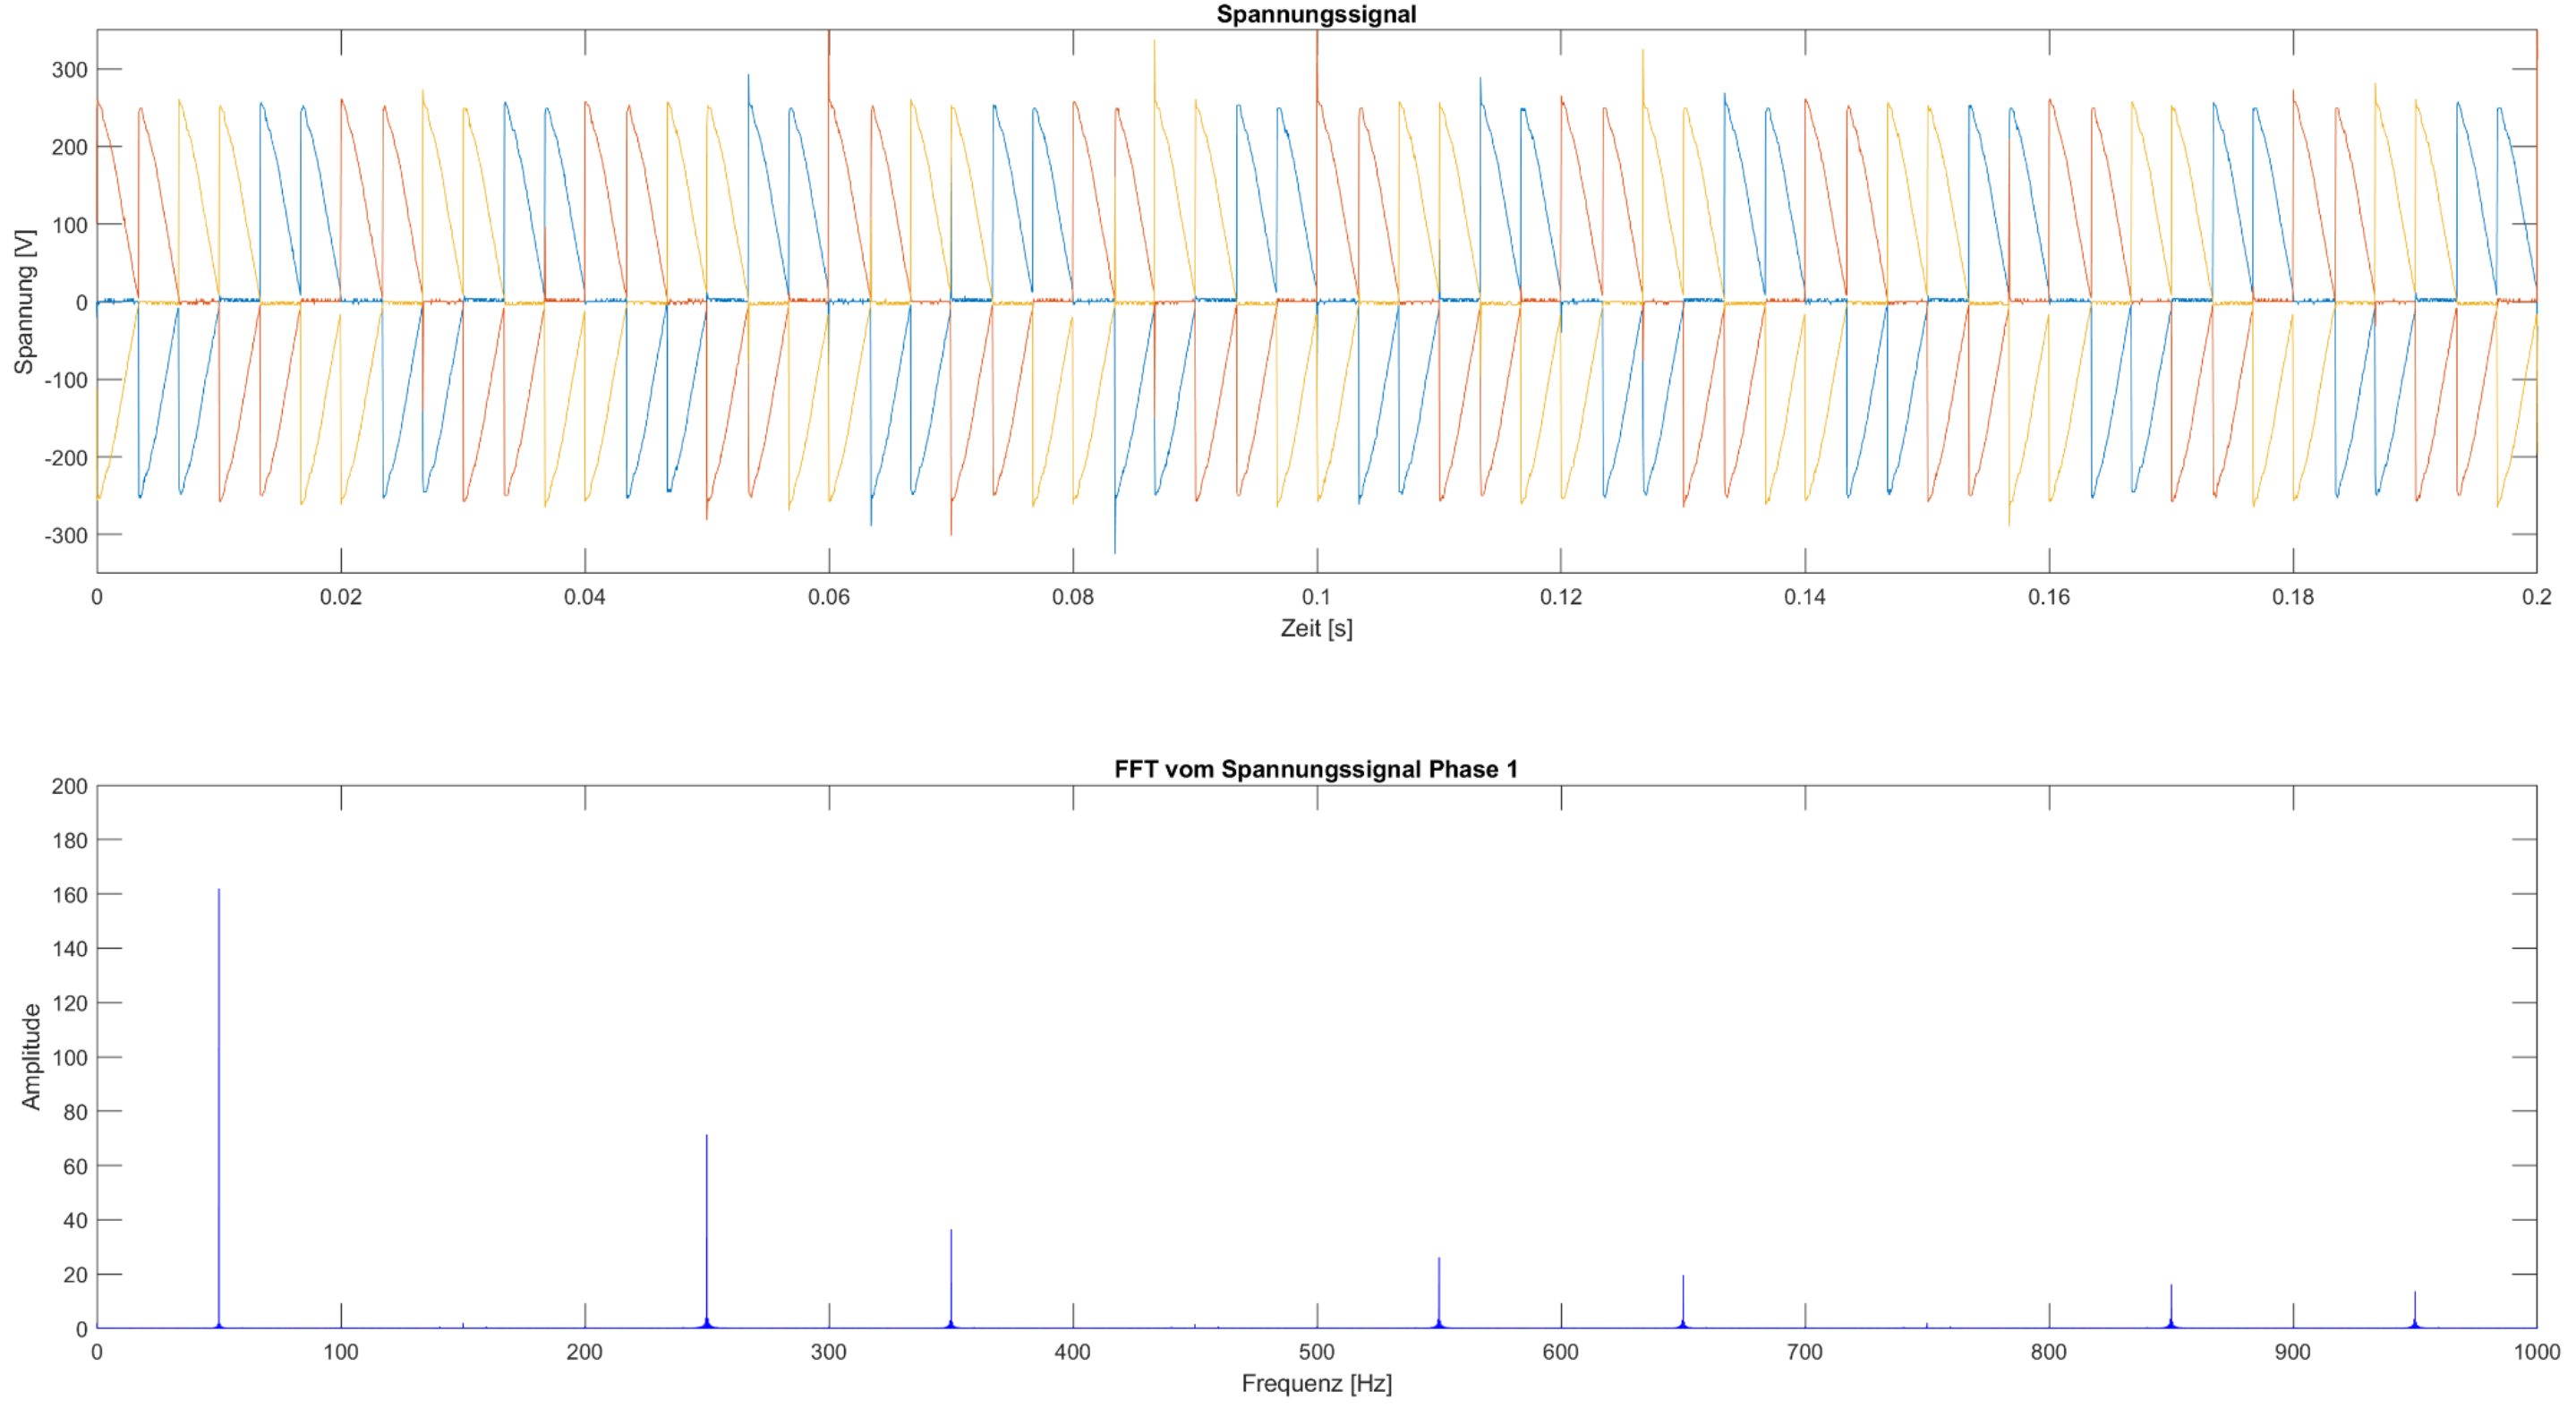
\includegraphics[width=0.96\textwidth]{Messung_Widerstand_Phas_90grad.png}	
	\caption{Messung mit Phasenanschnitt 90\textdegree}\label{fig:Mess_Phas_90}
\end{figure}

\newpage
\subsection{Messungen Spannungen ASM}\label{sec:Mess_Spannung_ASM}
\subsubsection*{Schwingungspaket mit einem Duty Cycle von 0.5}
\begin{figure}[ht!]
	\centering
	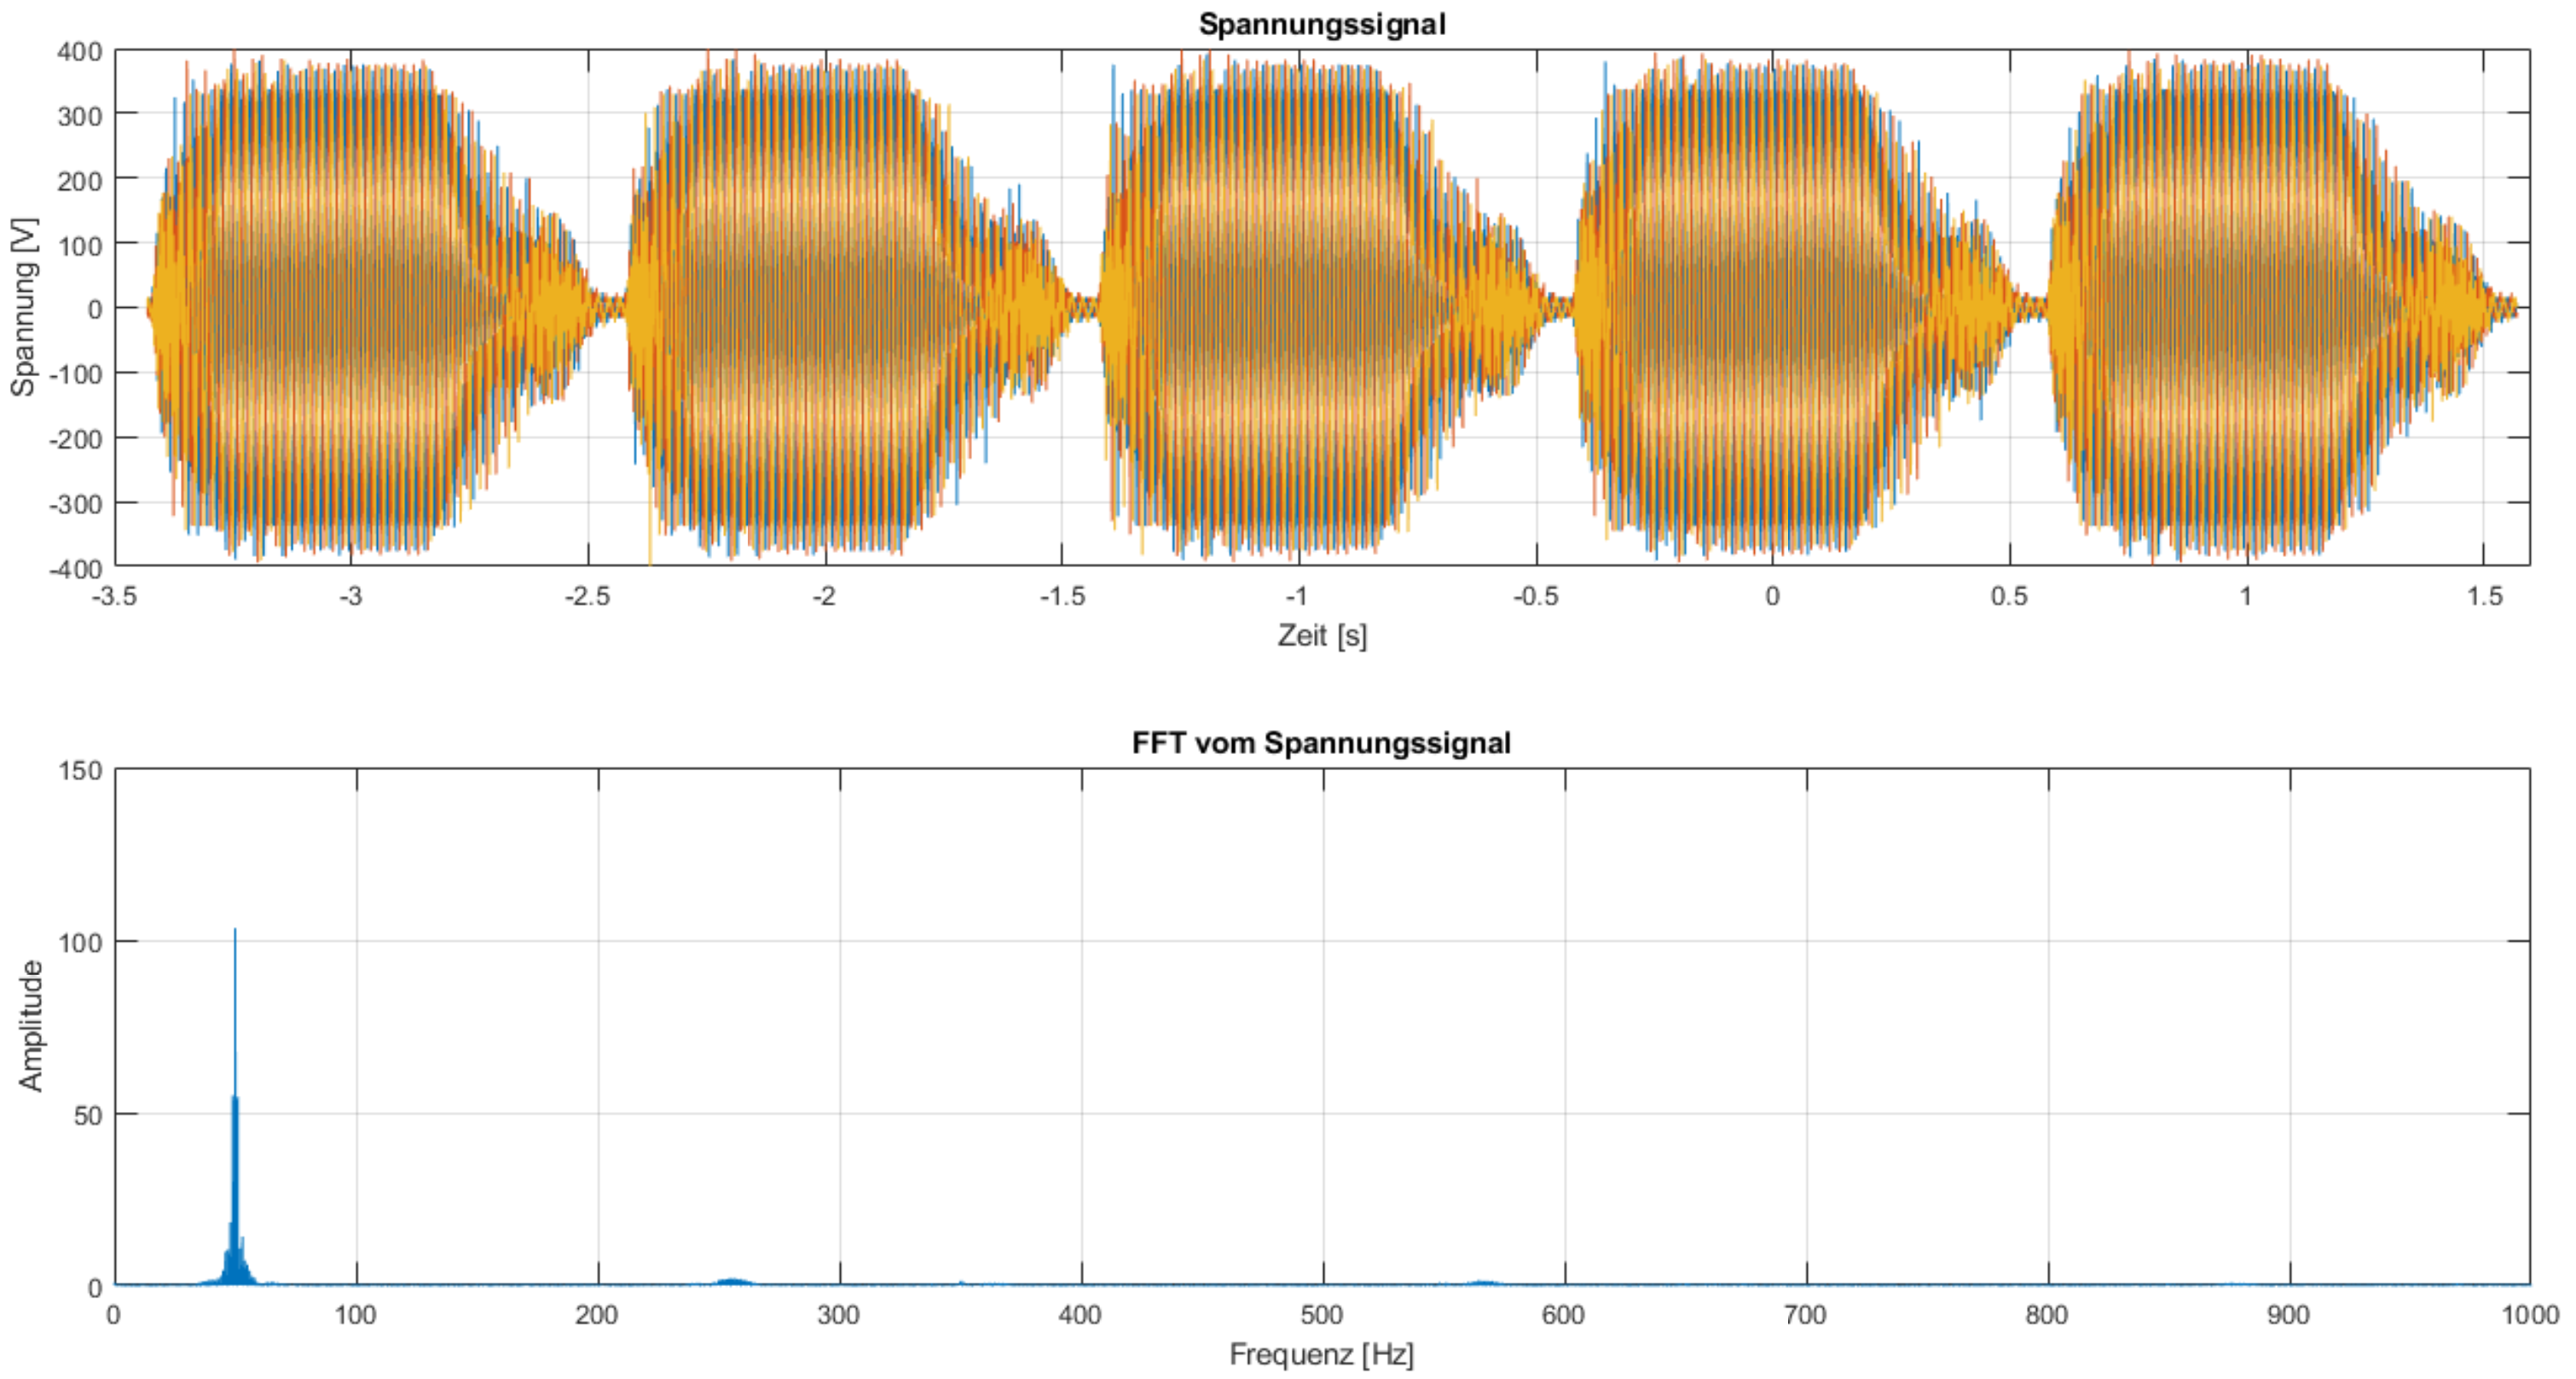
\includegraphics[width=0.96\textwidth]{Messung_ASM_Schwing_0_5.png}	
	\caption{Messung mit Schwingungspaket mit einem Duty Cycle von 0.5}\label{fig:Mess_ASM_Schwing_0_5}
\end{figure}

\subsubsection*{Schwingungspaket mit einem Duty Cycle von 0.8}
\begin{figure}[ht!]
	\centering
	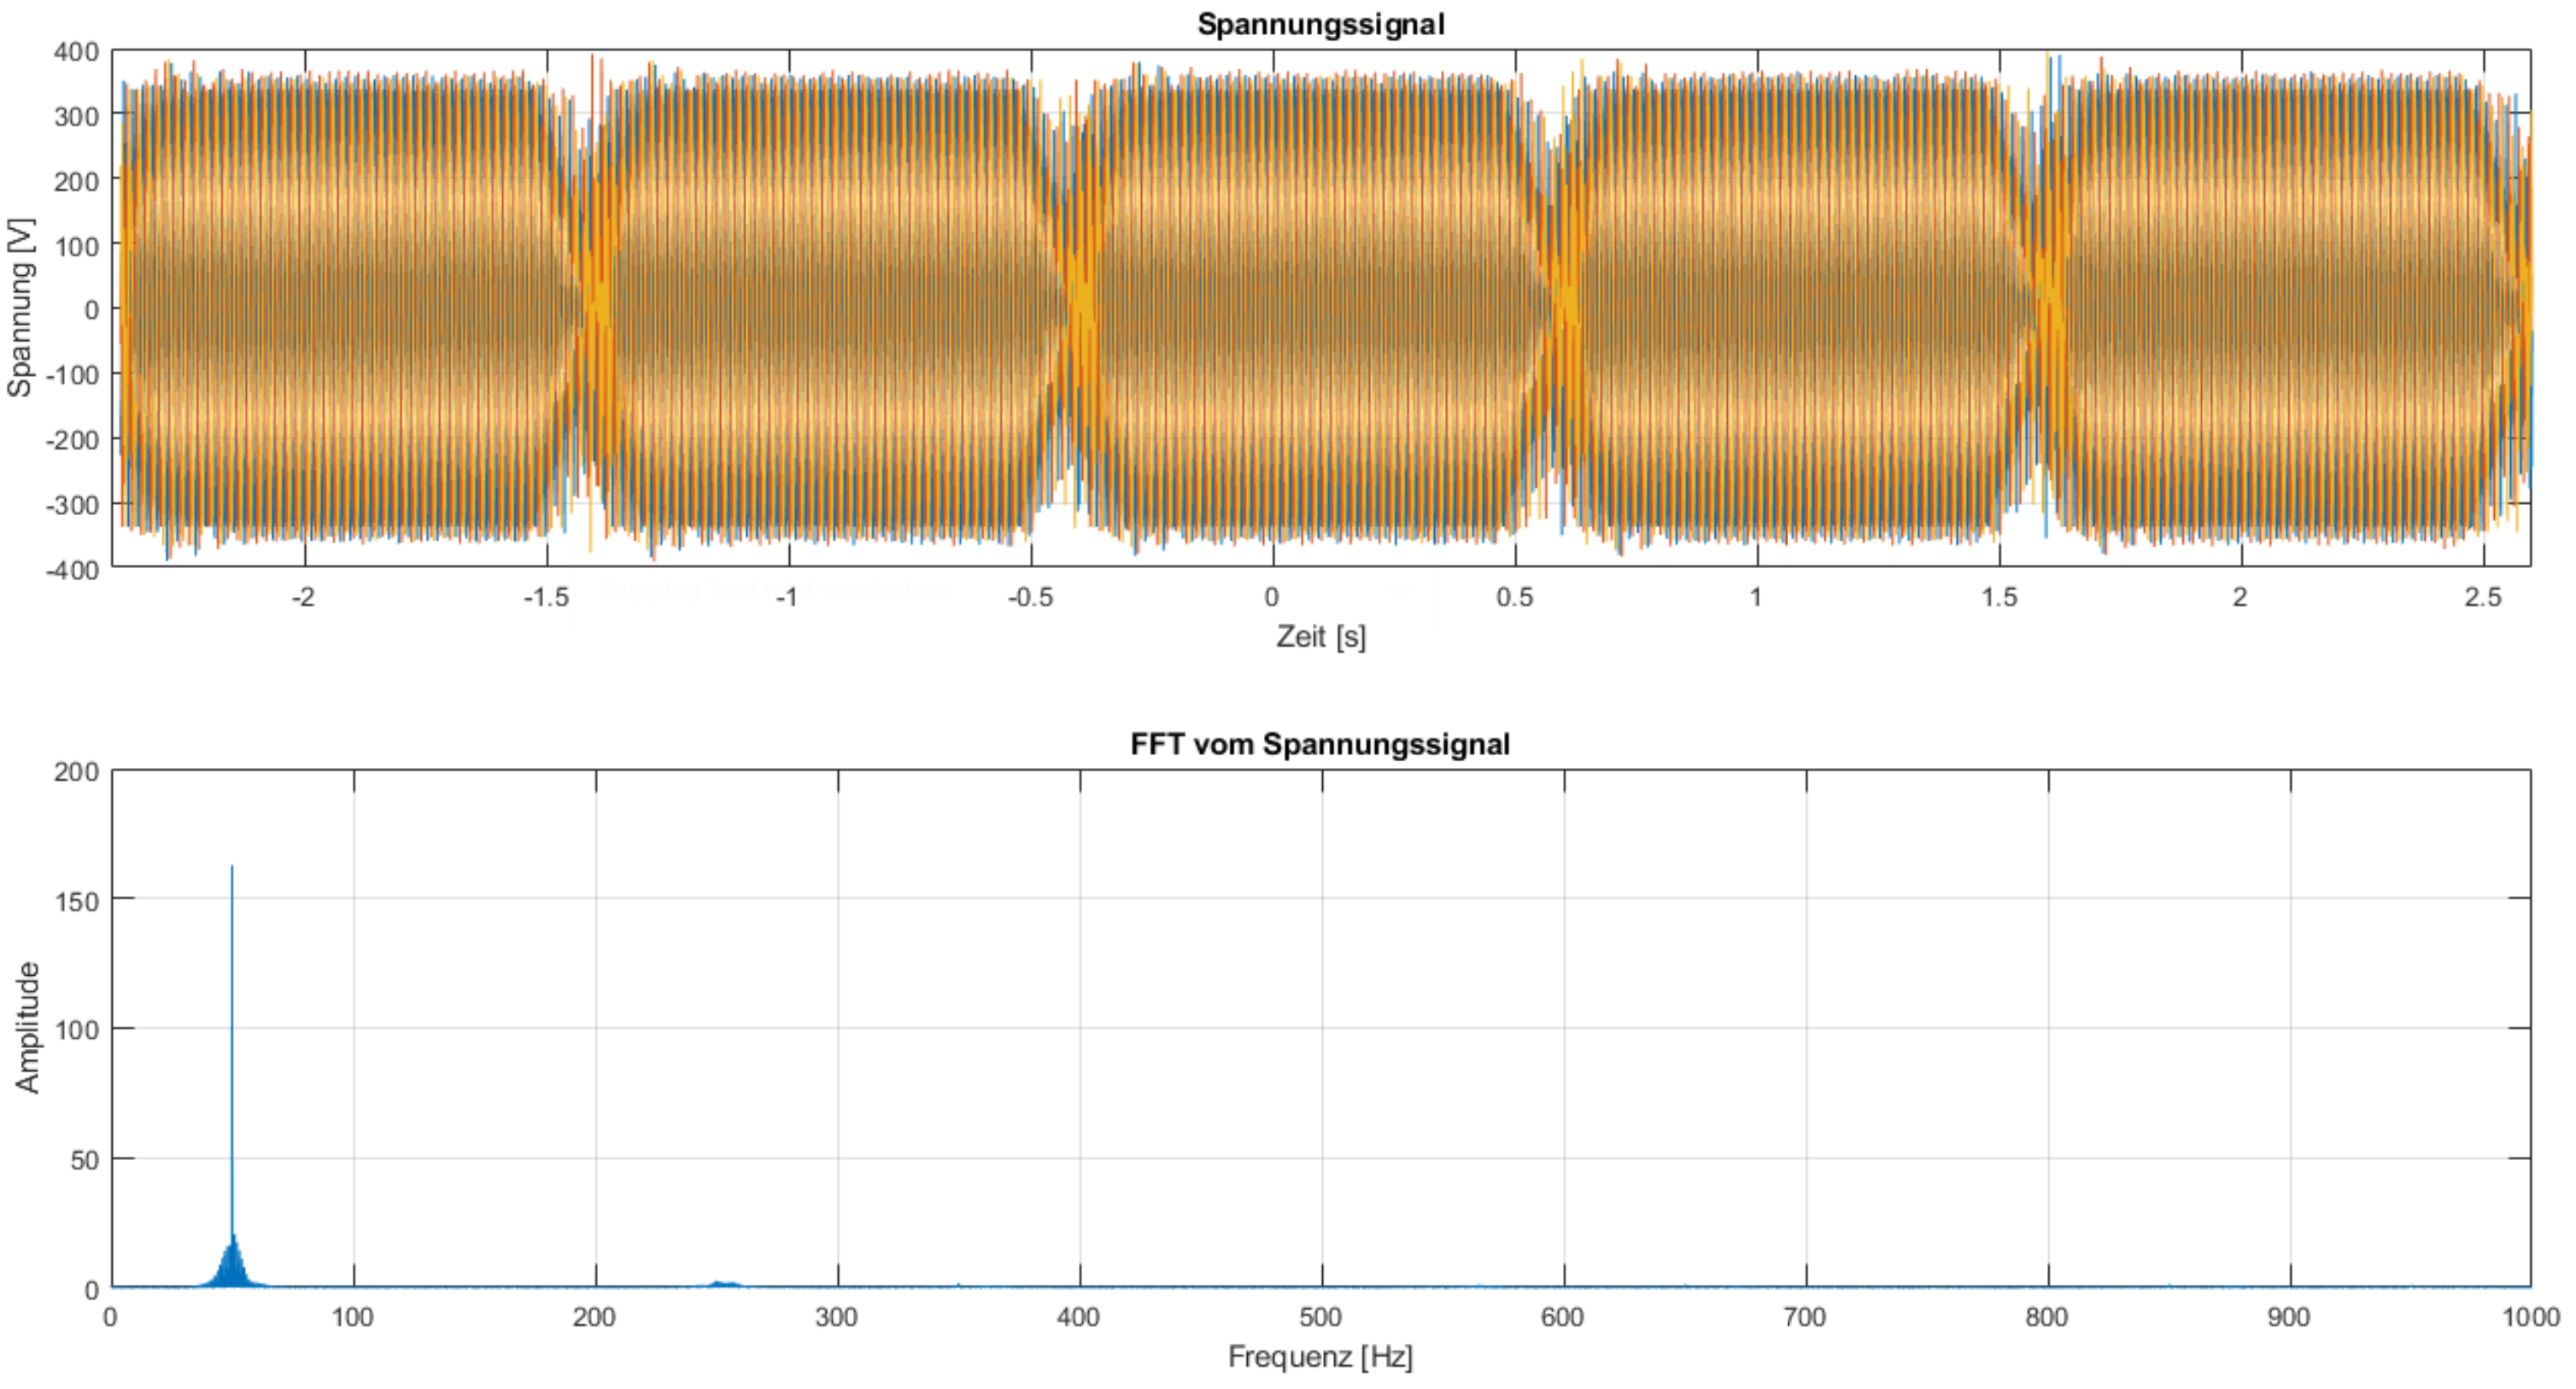
\includegraphics[width=0.96\textwidth]{Messung_ASM_Schwing_0_8.png}	
	\caption{Messung mit Schwingungspaket mit einem Duty Cycle von 0.8}\label{fig:Mess_ASM_Schwing_0_8}
\end{figure}
\newpage
\subsubsection*{Auf- und Absteuern}
\begin{figure}[ht!]
	\centering
	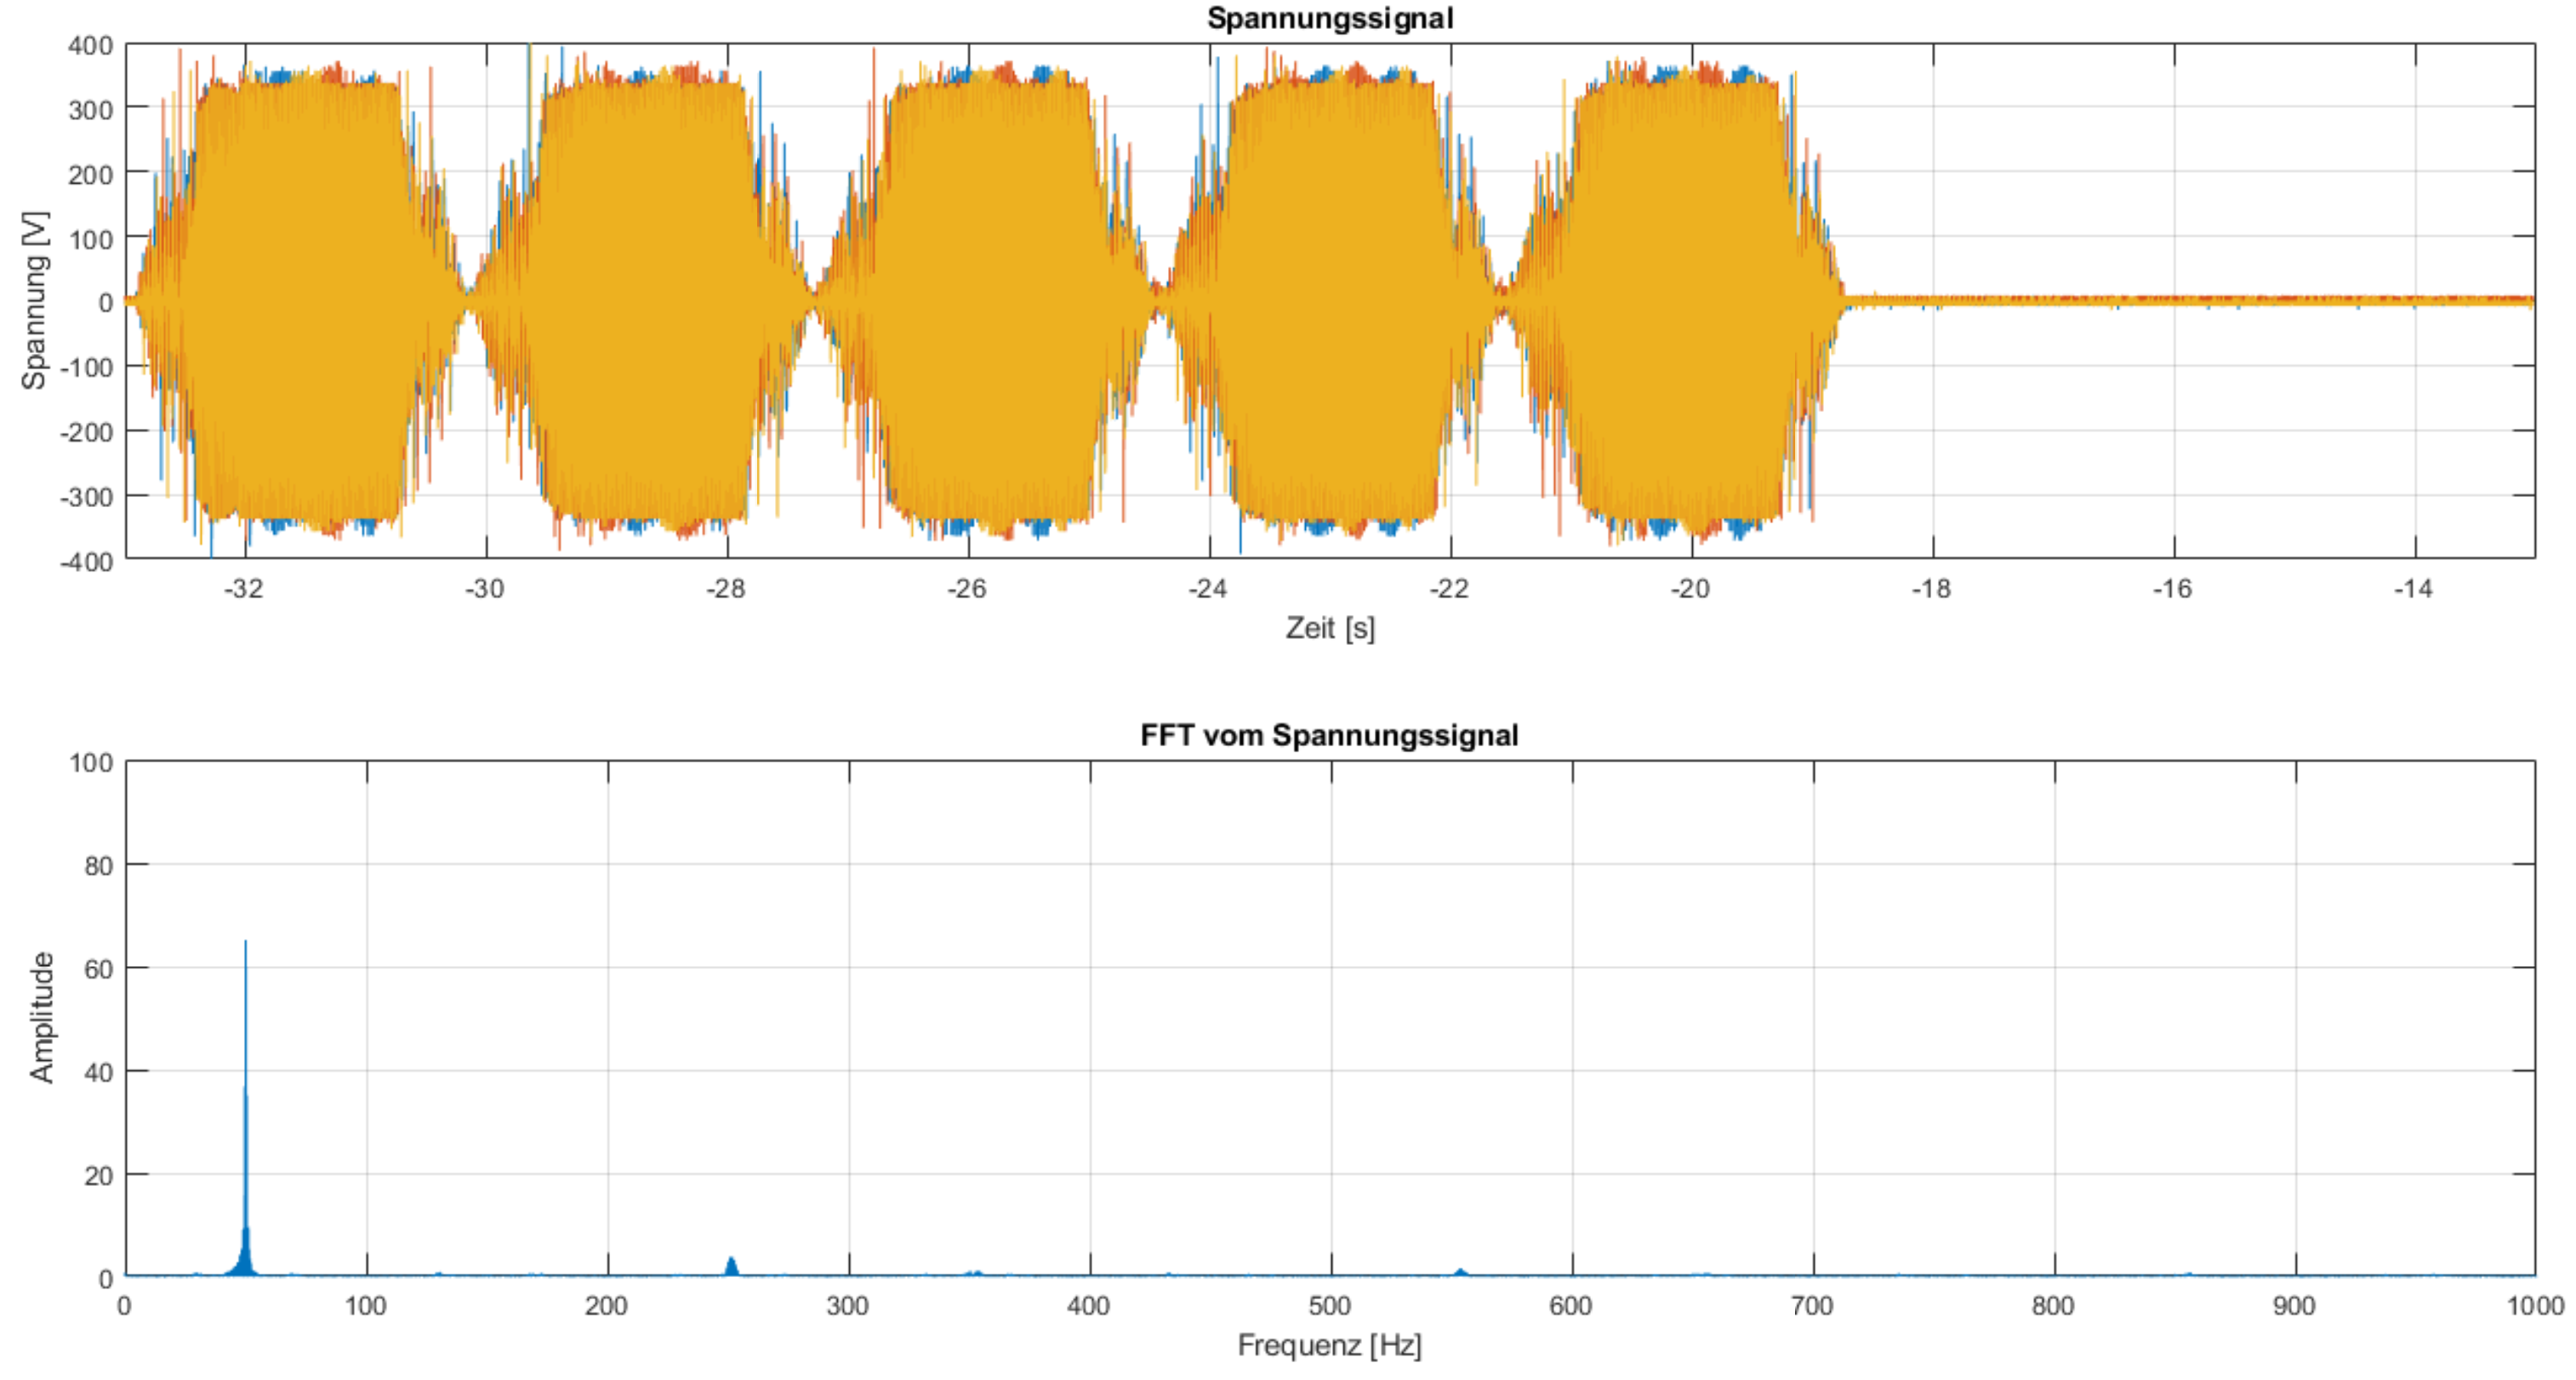
\includegraphics[width=0.96\textwidth]{Messung_ASM_Sanft.png}	
	\caption{Messung mit Sanft Anlasser}\label{fig:Mess_ASM_Sanft}
\end{figure}

\newpage
\subsection{Sparvariante für den Widerstand mit zwei Thyristoren} \label{sec:Sparvariante_2Thyristoren}
\subsubsection*{Phasenanschnitt 60\textdegree}

\begin{figure}[ht!]
	\centering
	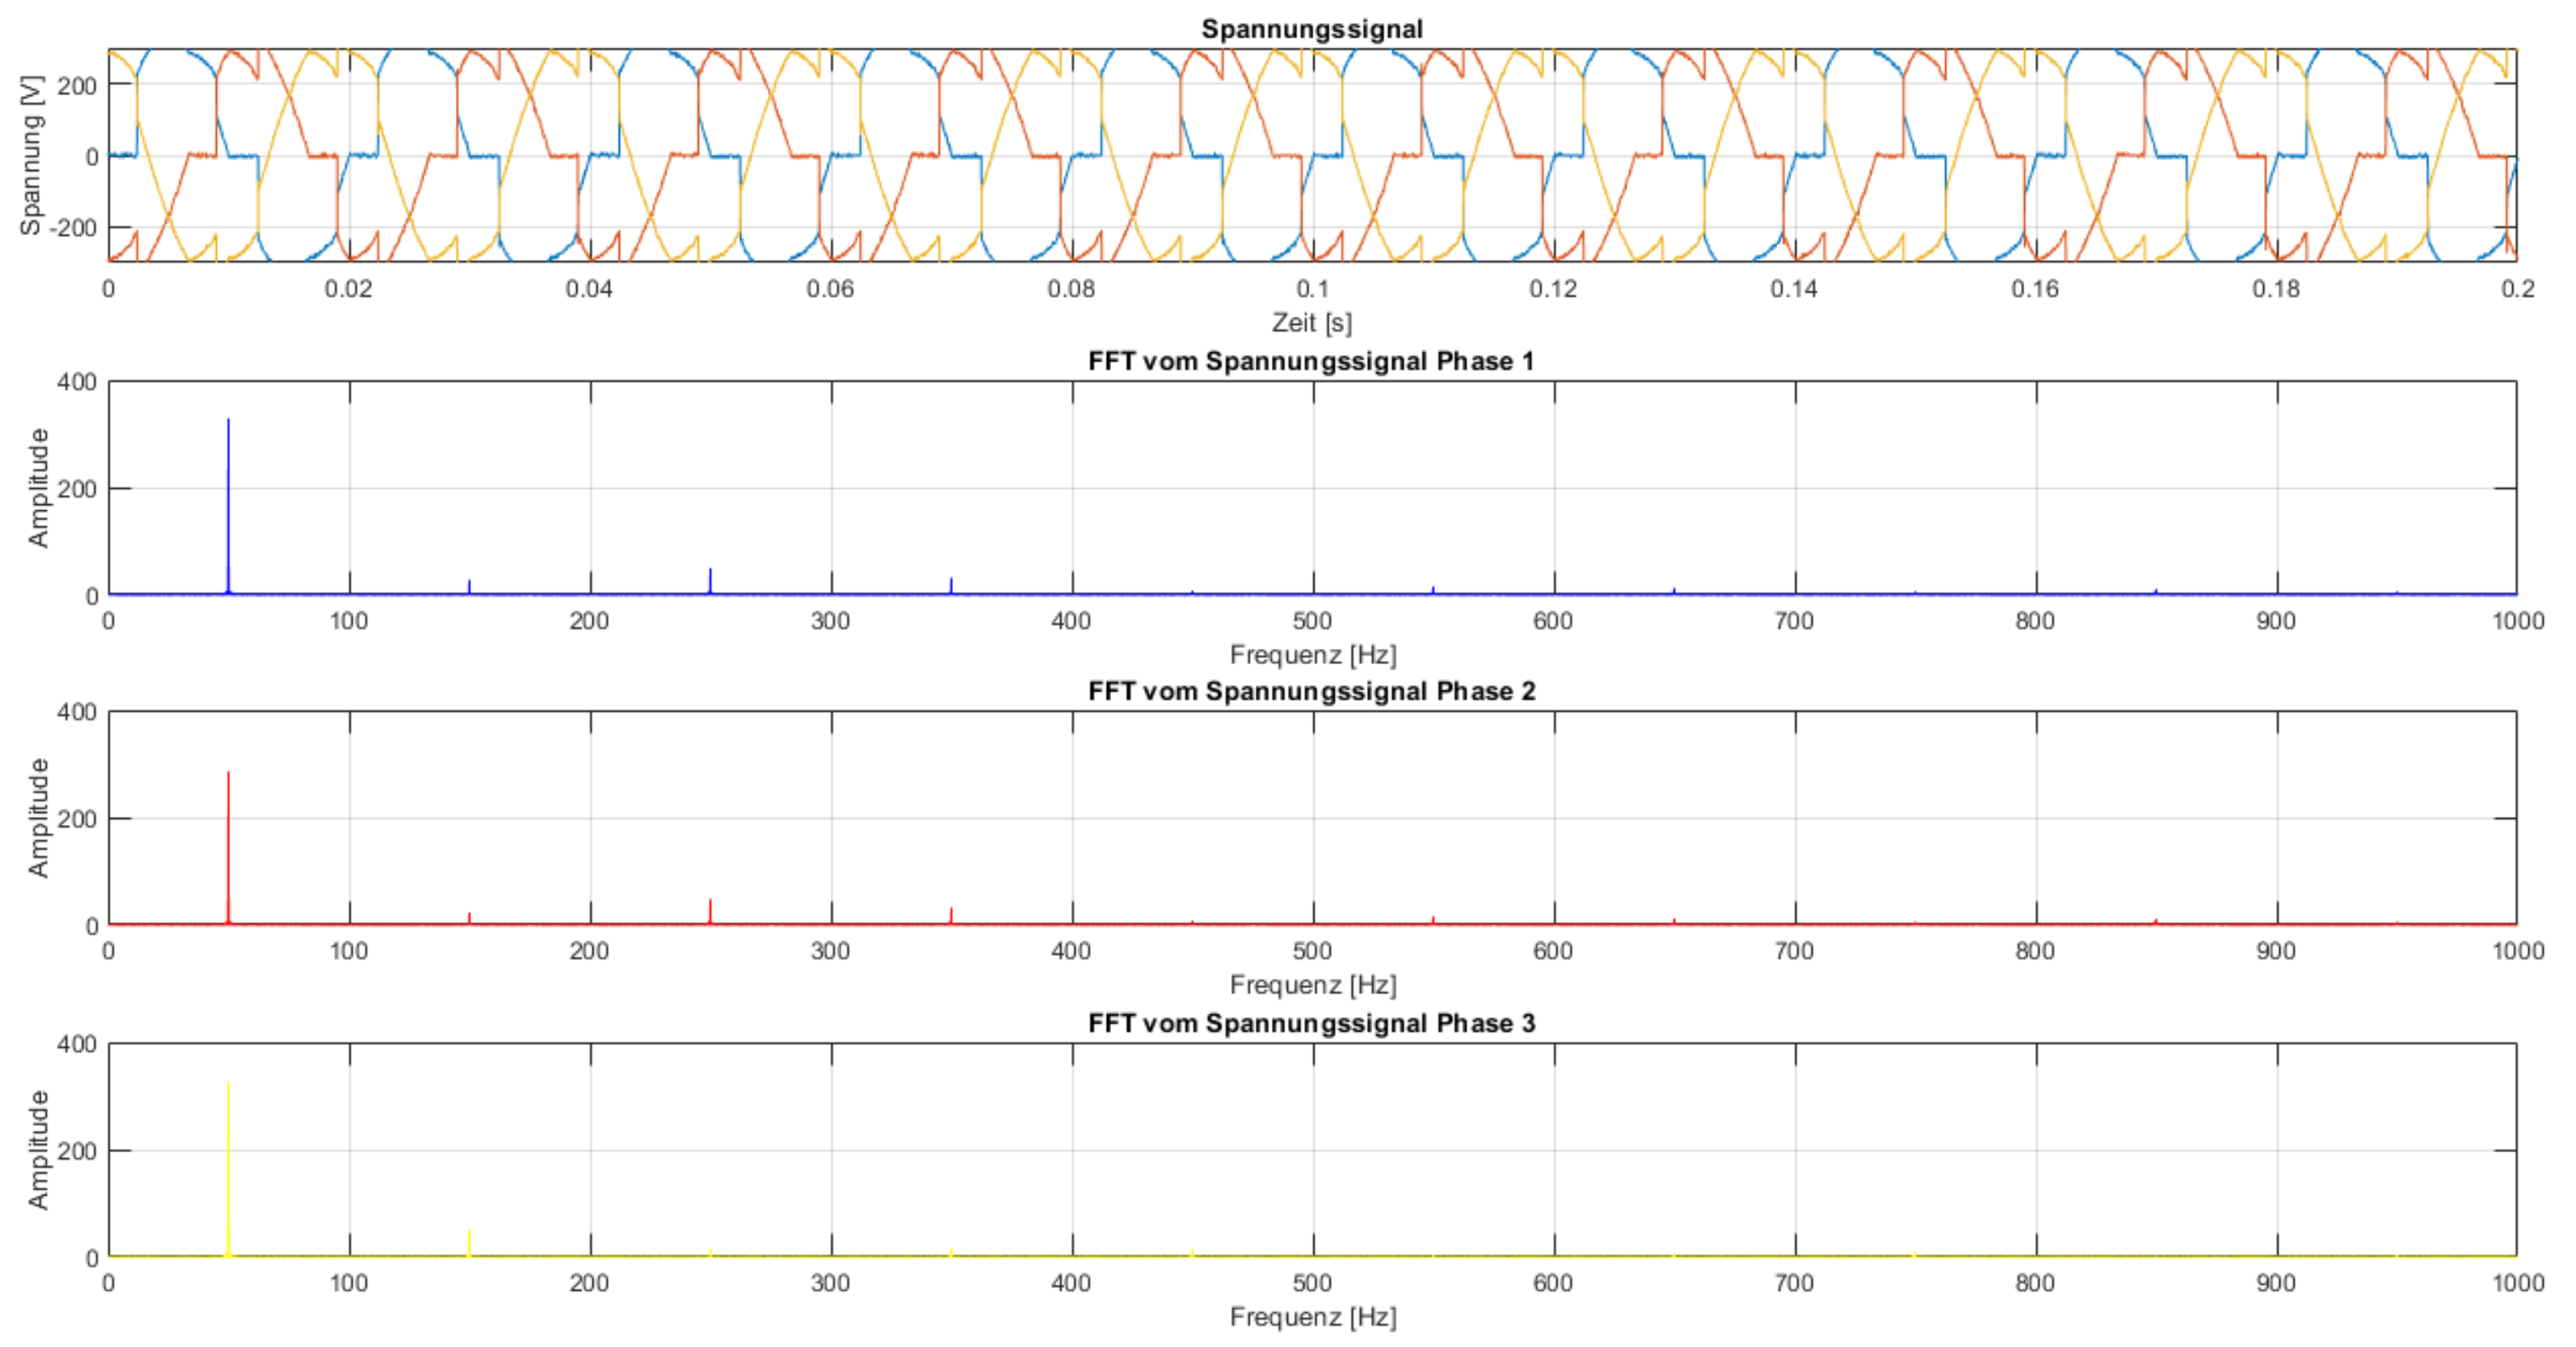
\includegraphics[width=0.96\textwidth]{Mess_2Thyristoren_Widerstand_Phas_60.png}	
	\caption{Messung mit Phasenanschnitt 60\textdegree \hspace{0.02cm} und zwei Thyristoren}\label{fig:Mess_2Thyristoren_Phas_60grad}
\end{figure}

\subsubsection*{Phasenanschnitt 90\textdegree}

\begin{figure}[ht!]
	\centering
	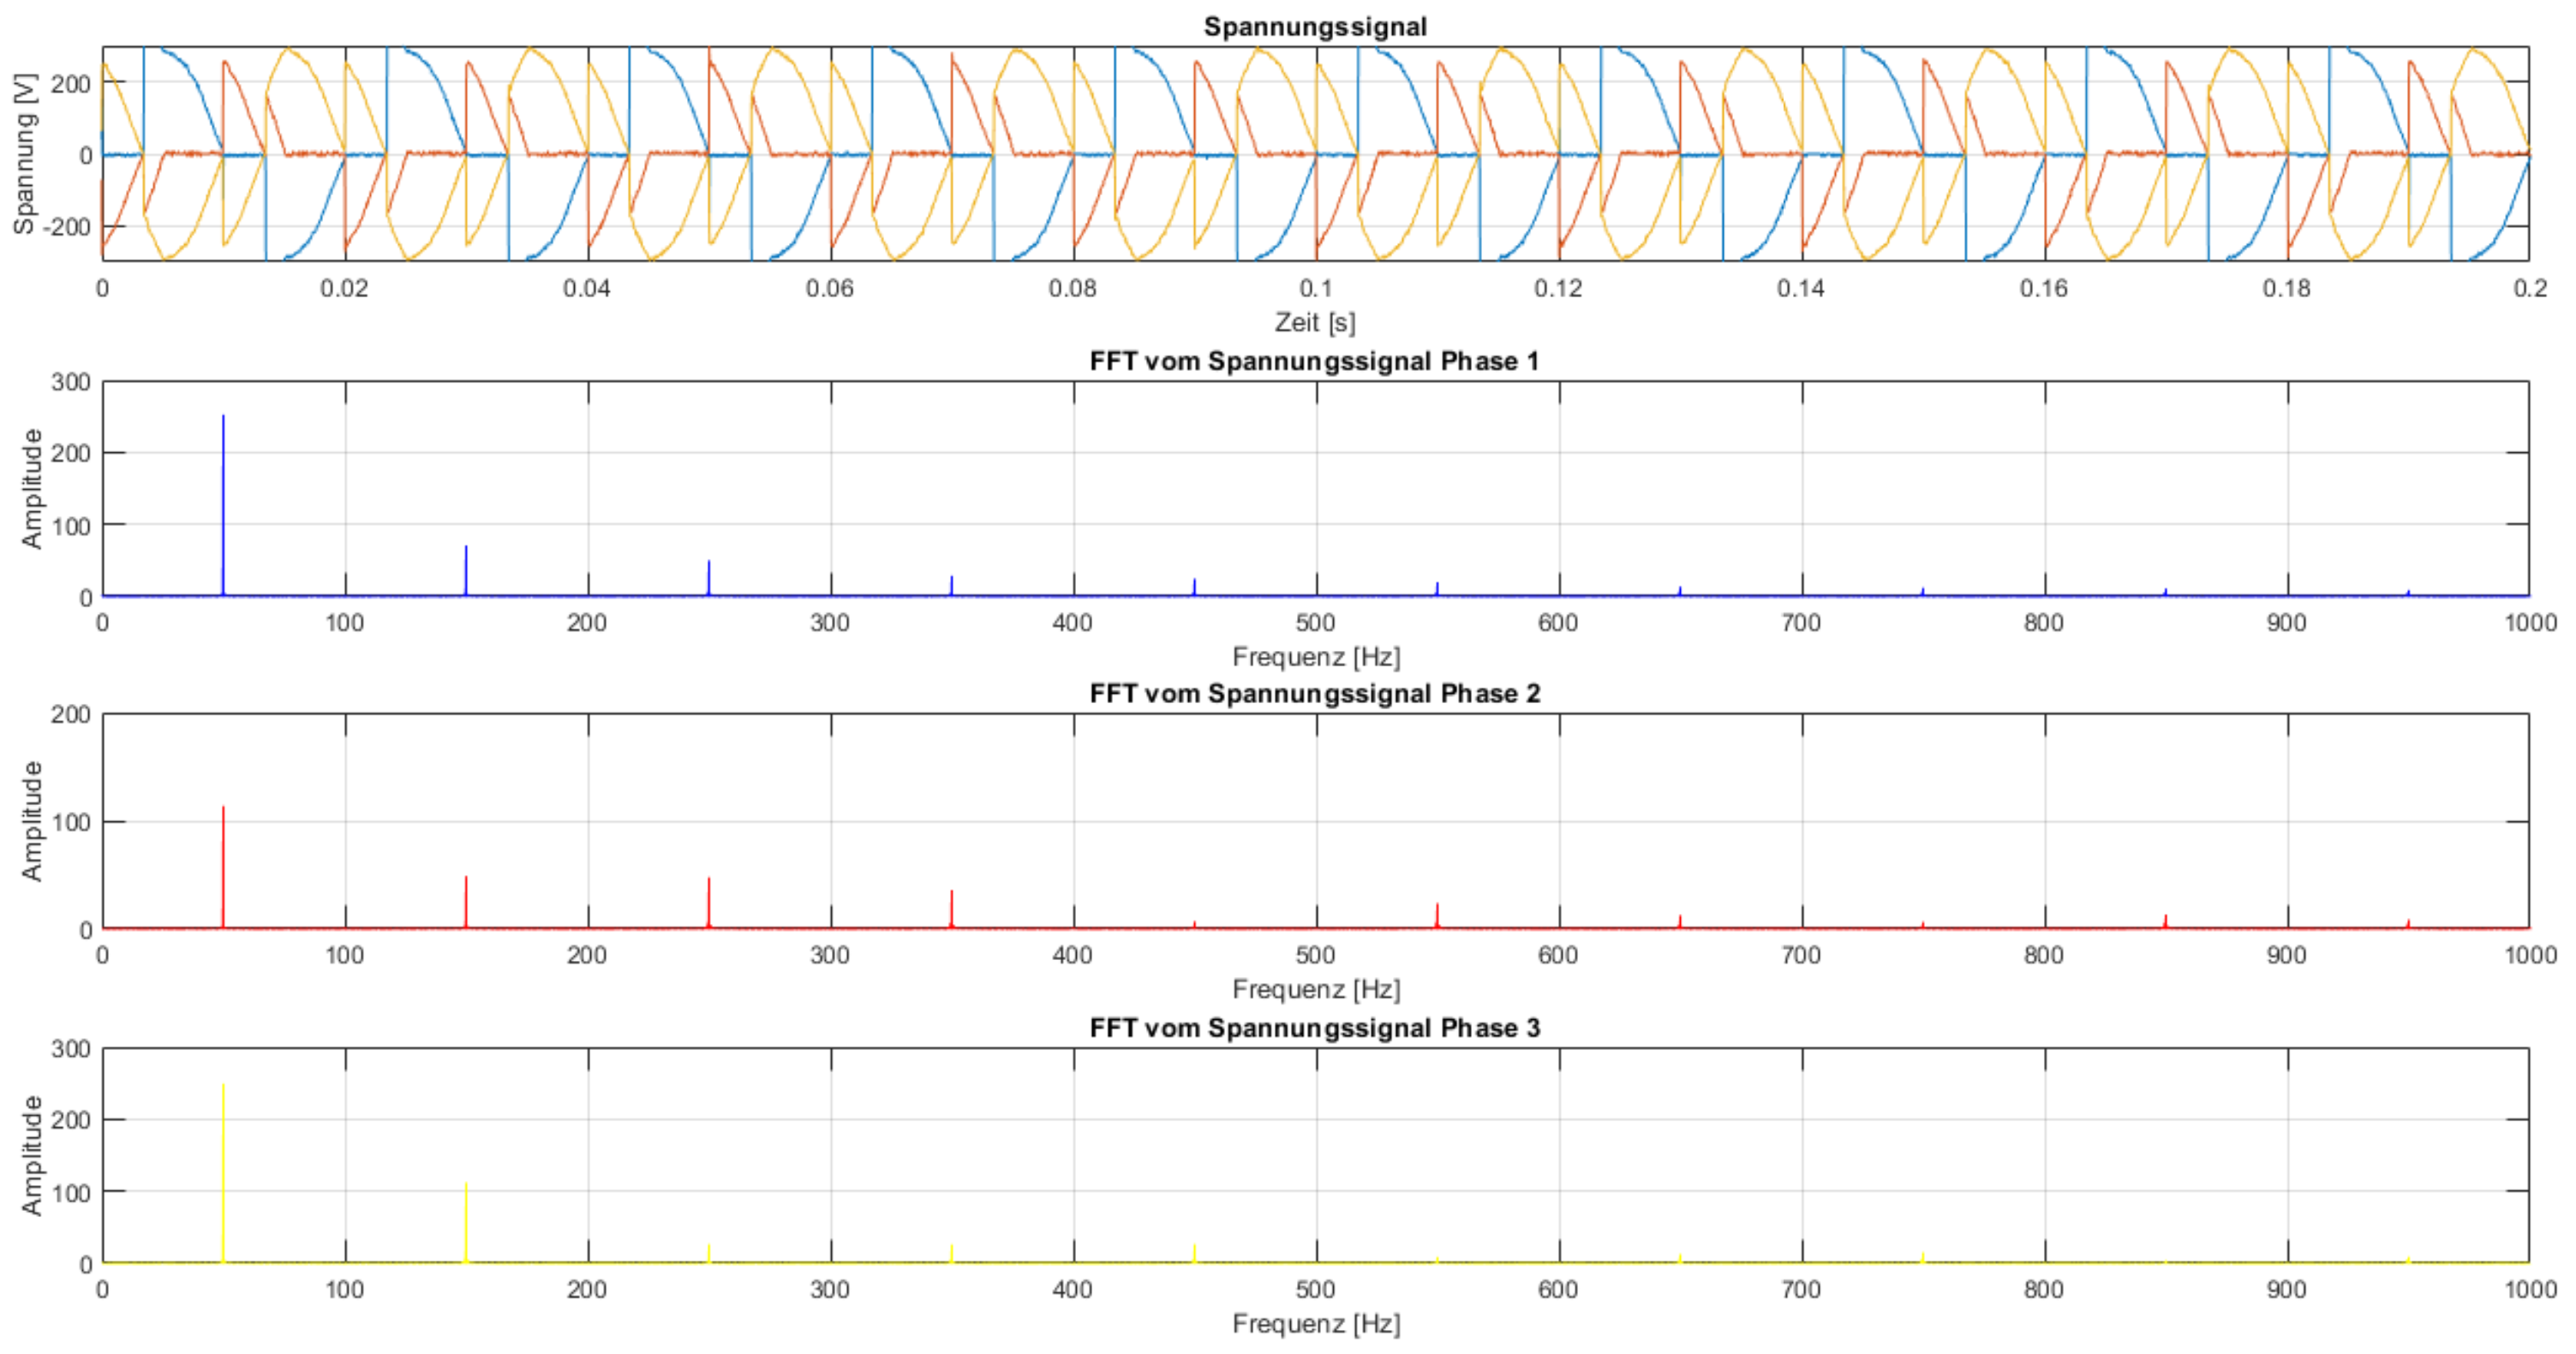
\includegraphics[width=0.96\textwidth]{Mess_2Thyristoren_Widerstand_Phas_90.png}	
	\caption{Messung mit Phasenanschnitt 90\textdegree \hspace{0.02cm} und zwei Thyristoren}\label{fig:Mess_2Thyristoren_Phas_90grad}
\end{figure}

\newpage
\subsubsection*{Schwingungspaket mit einem Duty Cycle von 0.5}

\begin{figure}[ht!]
	\centering
	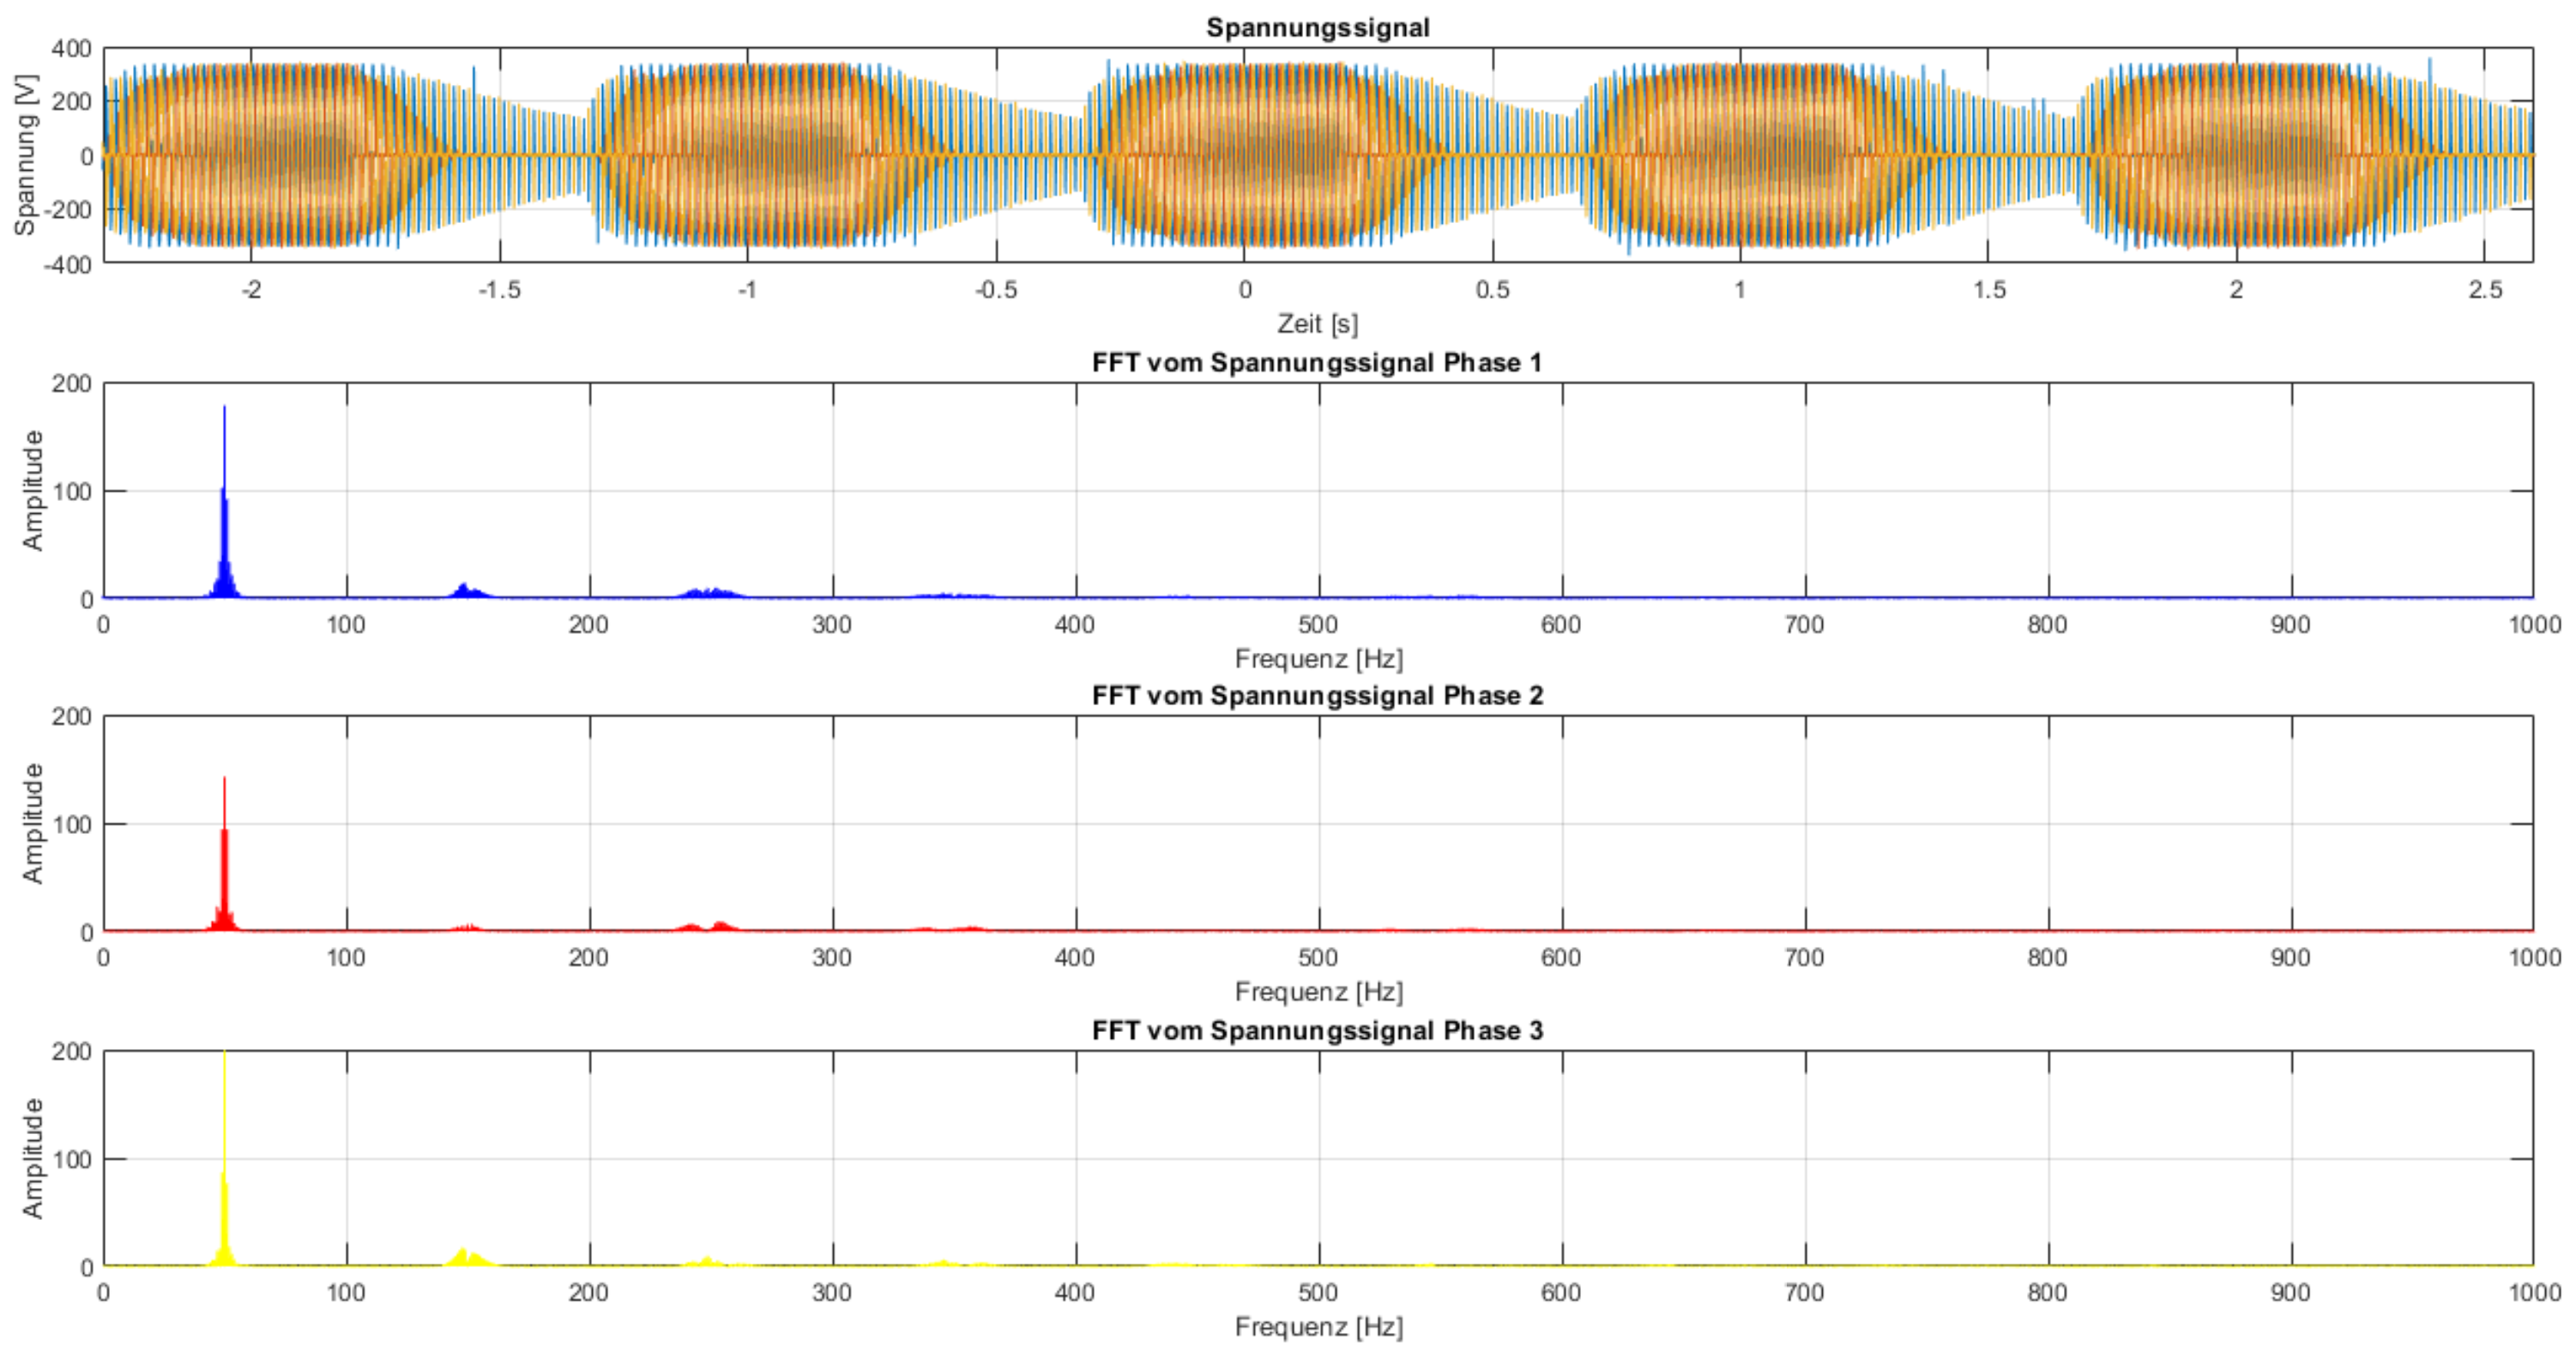
\includegraphics[width=0.96\textwidth]{Mess_2Thyristoren_Widerstand_Schwing_05.png}	
	\caption{Messung mit Schwingungspaket mit einem Duty Cycle von 0.5 und zwei Thyristoren}\label{fig:Mess_2Thyristoren_Schwing_50}
\end{figure}


\subsubsection*{Schwingungspaket mit einem Duty Cycle von 0.8}

\begin{figure}[ht!]
	\centering
	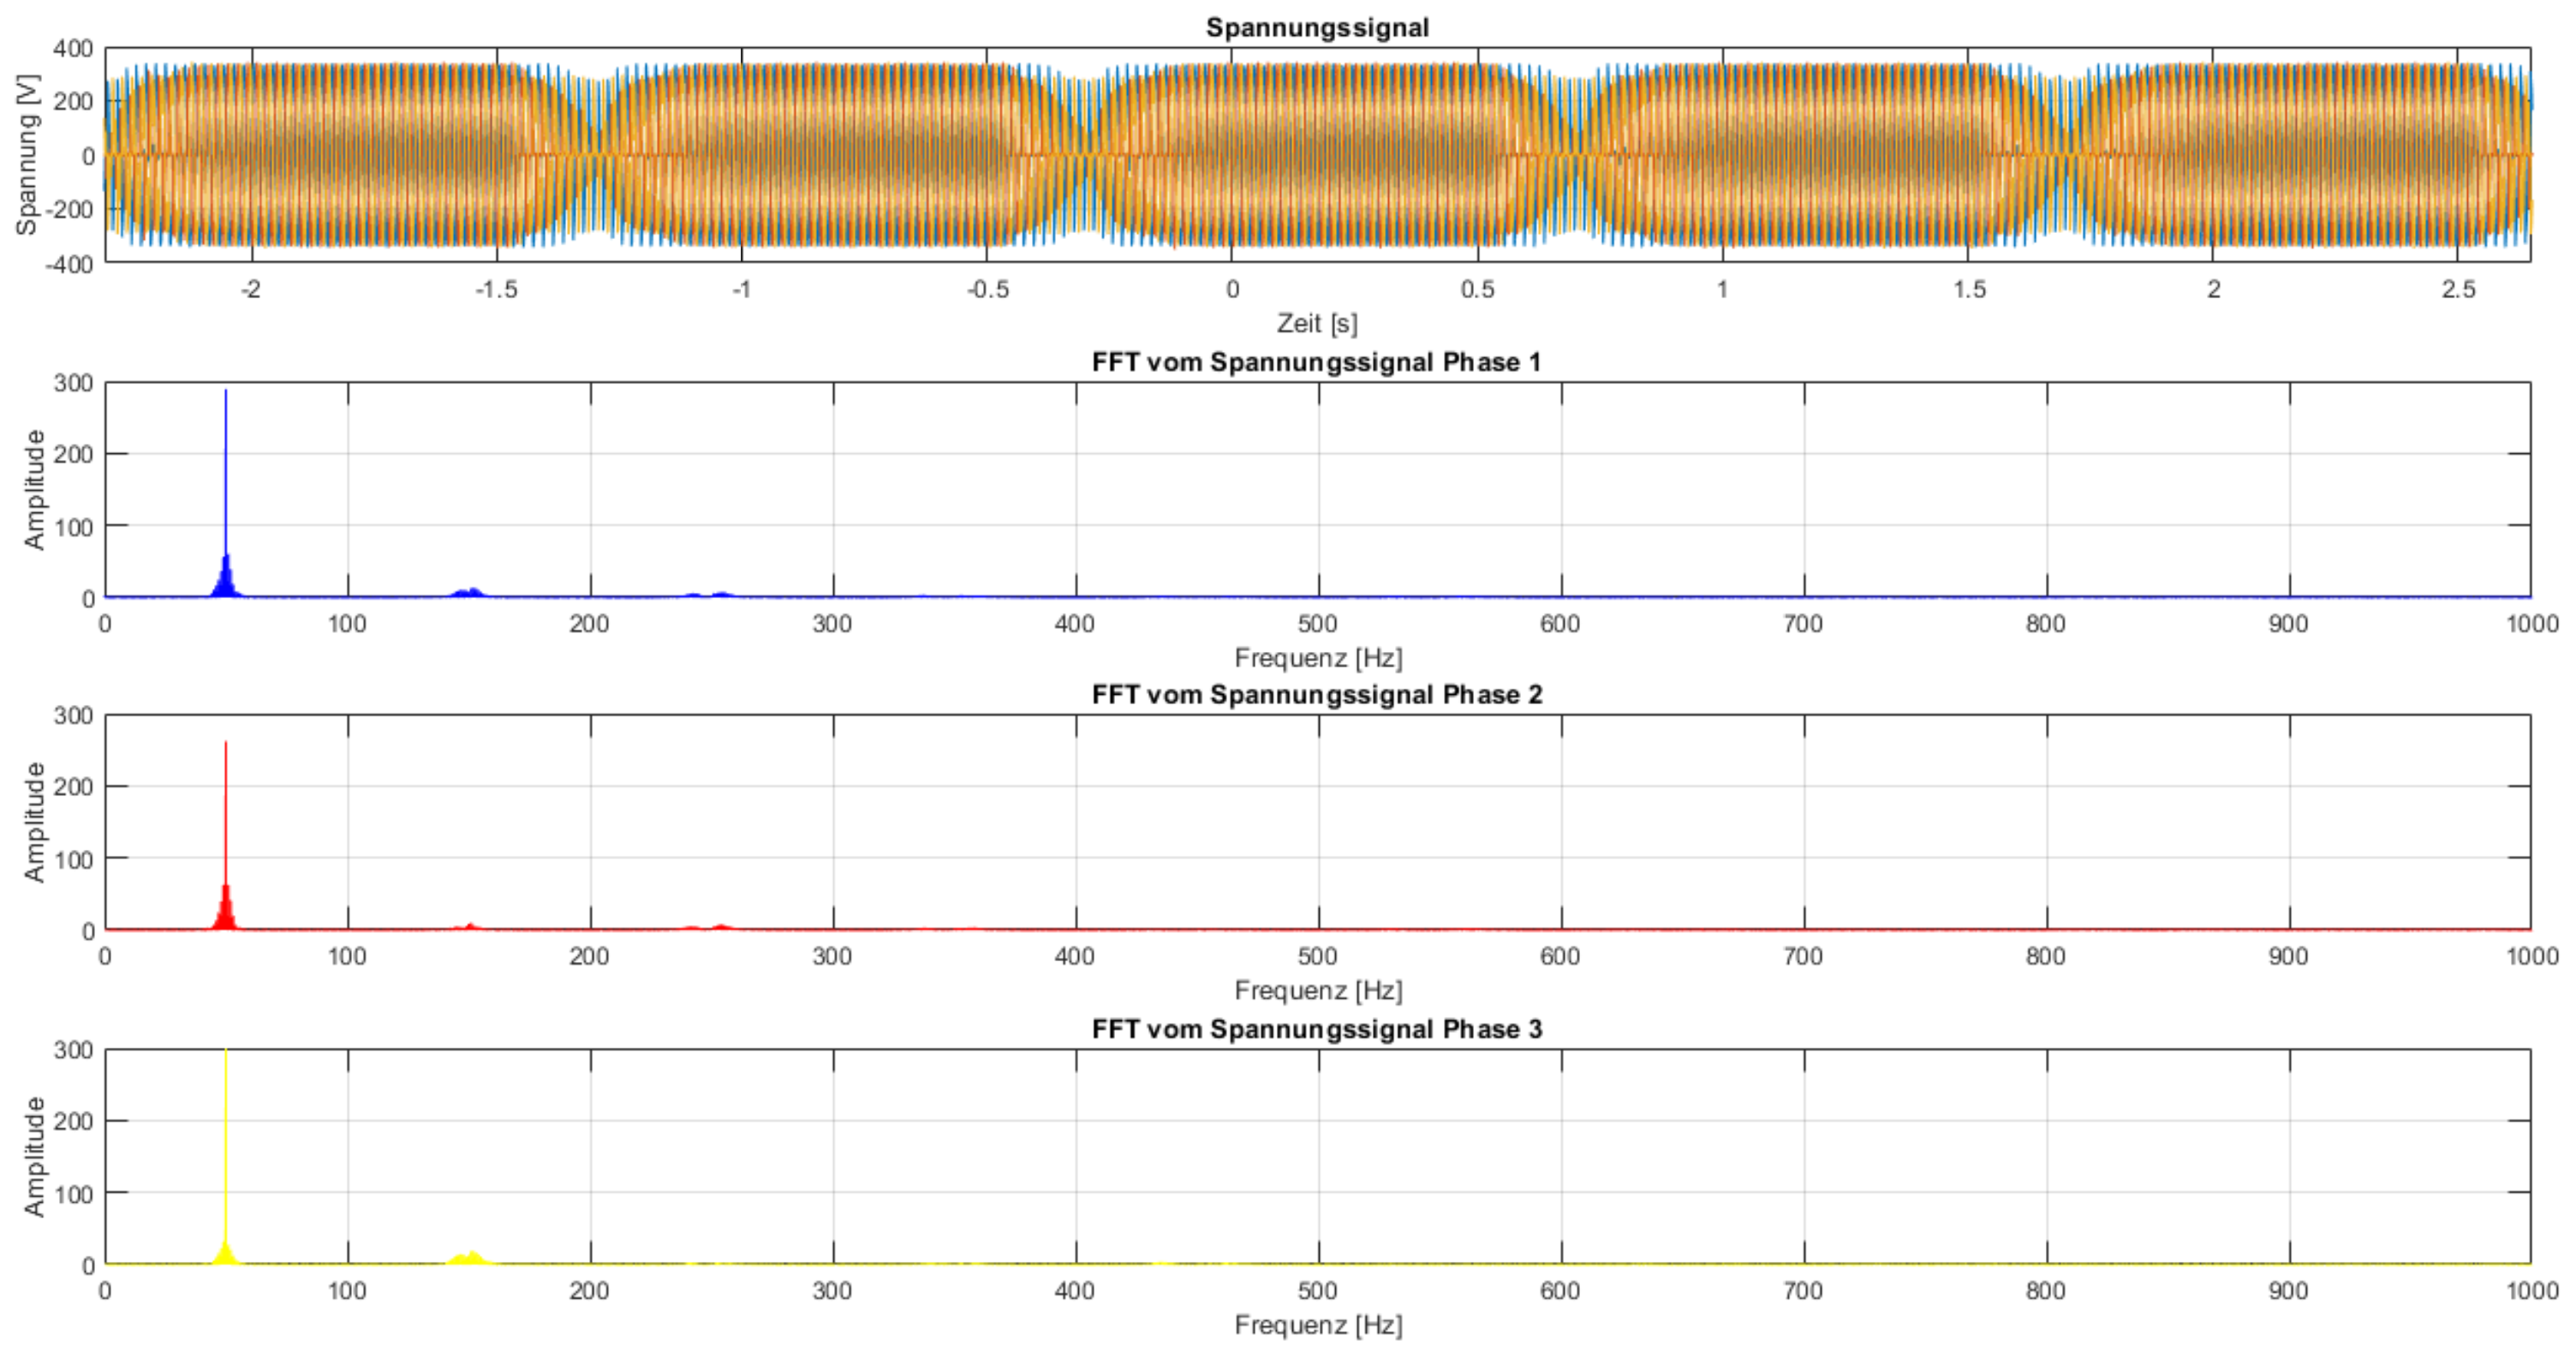
\includegraphics[width=0.96\textwidth]{Mess_2Thyristoren_Widerstand_Schwing_08.png}	
	\caption{Messung mit Schwingungspaket mit einem Duty Cycle von 0.8 und zwei Thyristoren}\label{fig:Mess_2Thyristoren_Schwing_80}	
\end{figure}

\newpage
\subsubsection*{Hartes Auf- und Absteuern}

\begin{figure}[ht!]
	\centering
	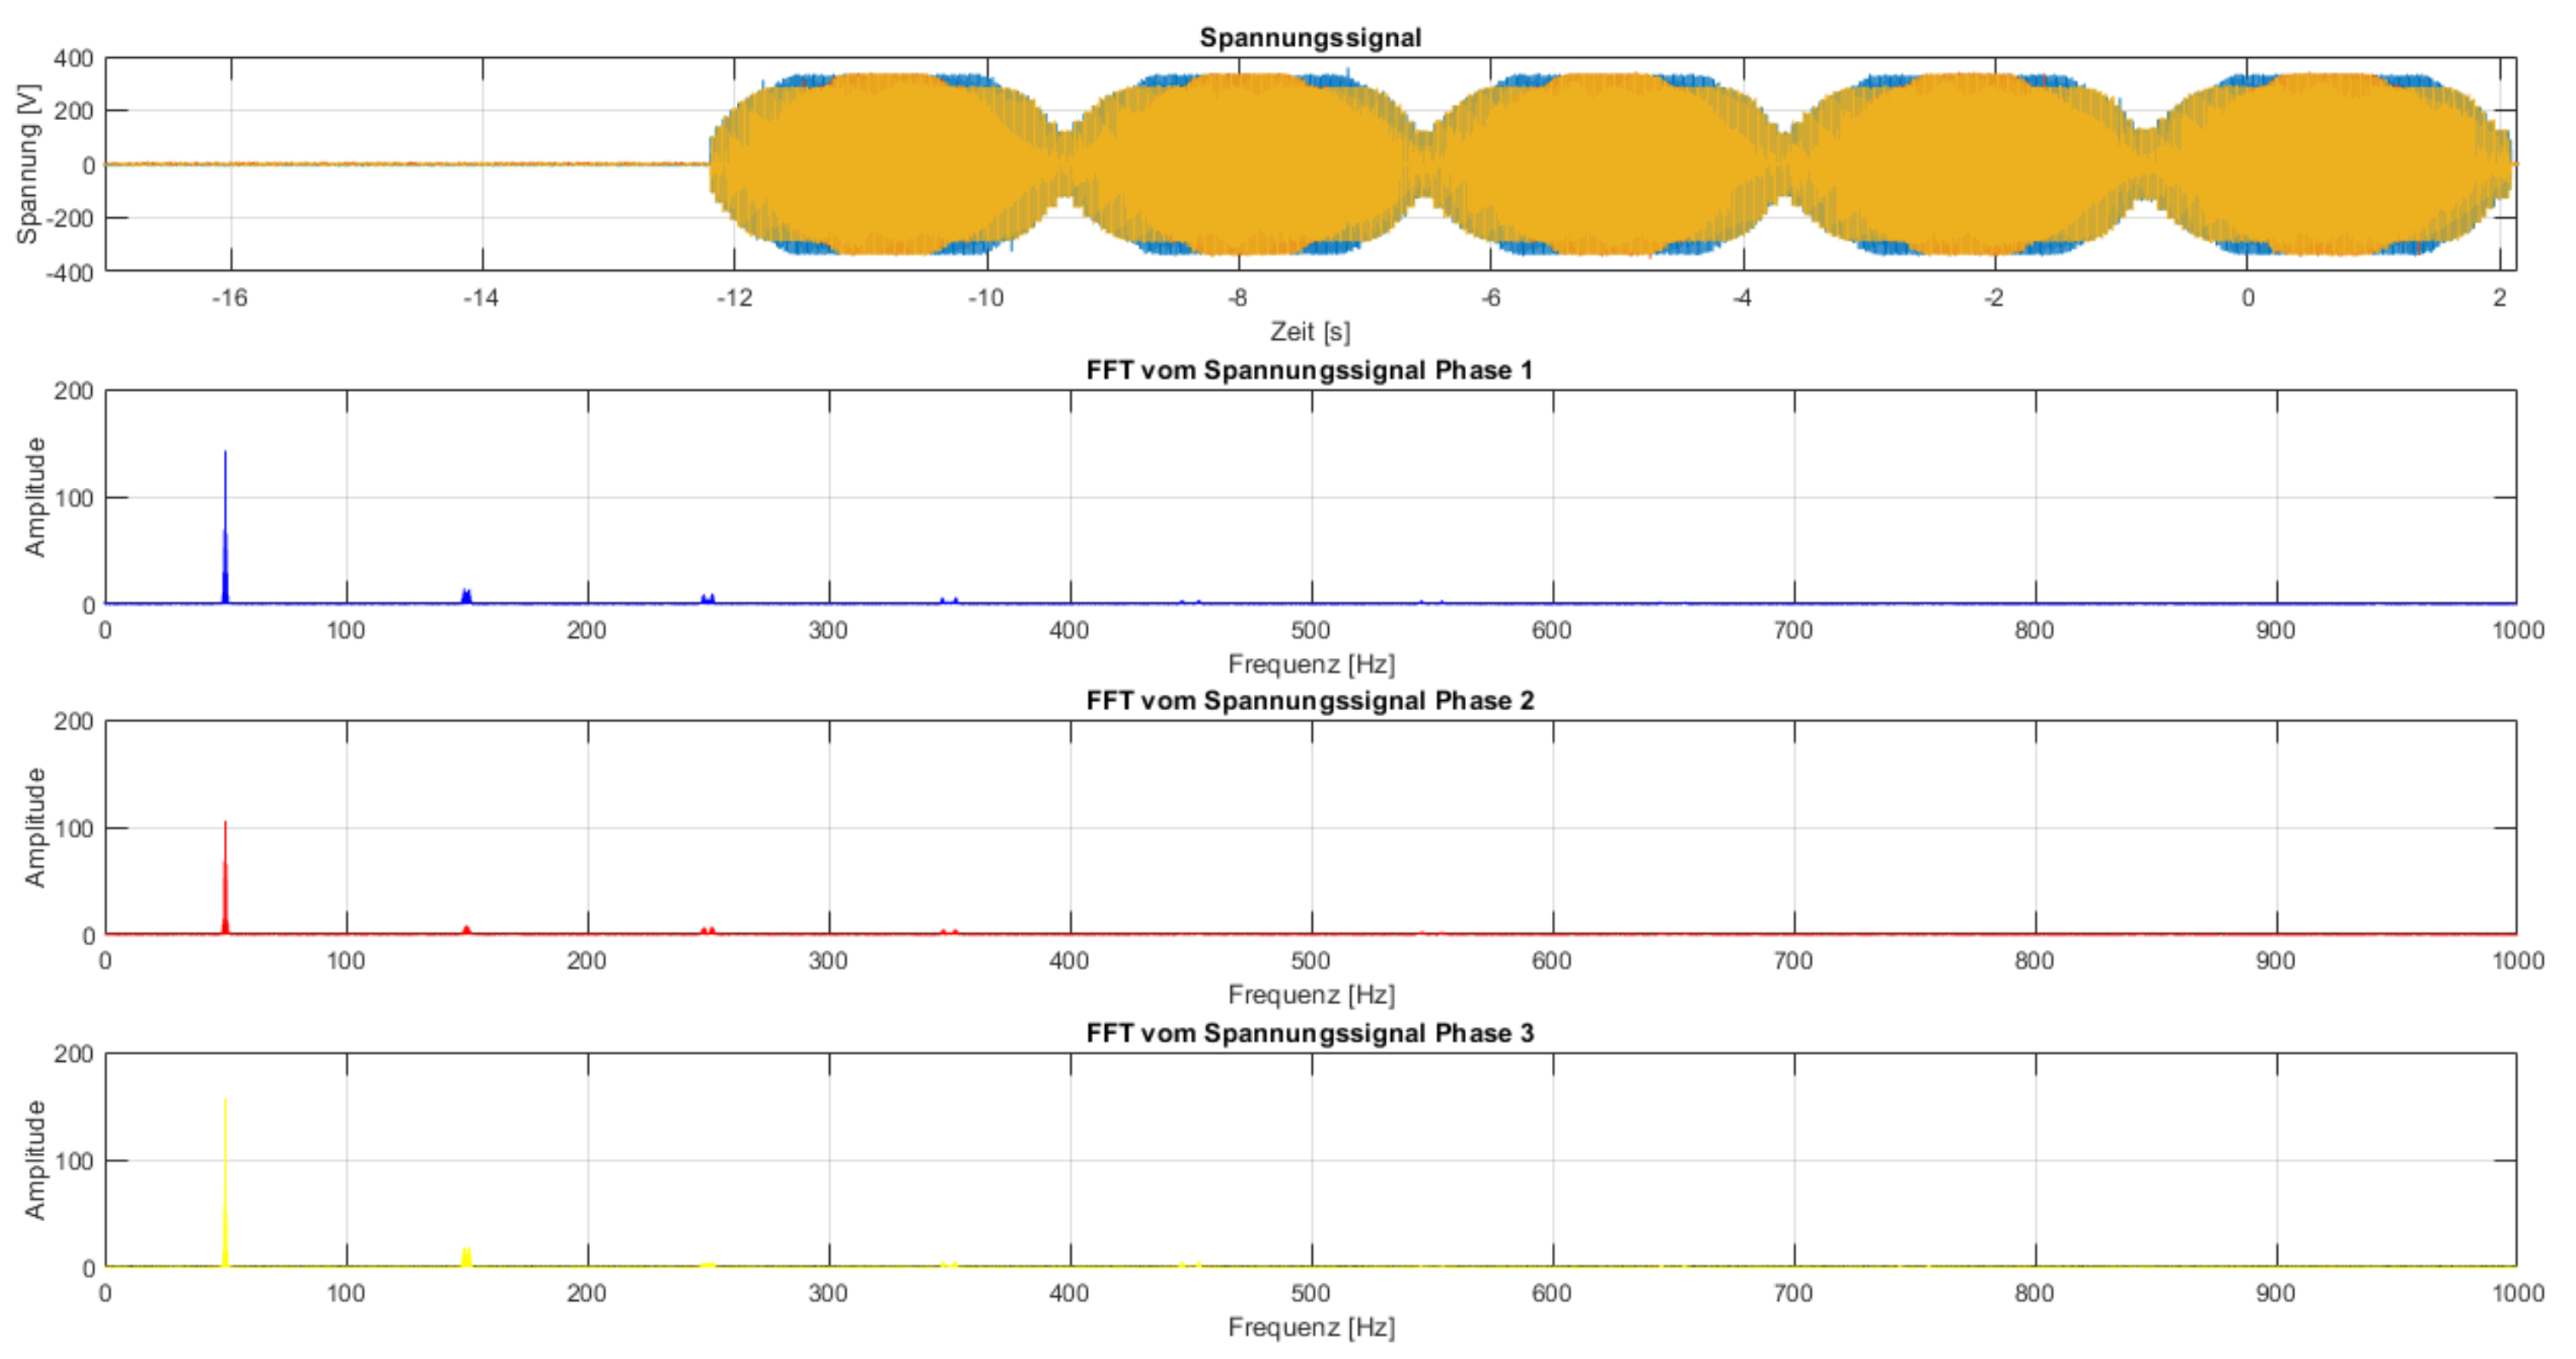
\includegraphics[width=0.96\textwidth]{Mess_2Thyristoren_Widerstand_AufAbFahren.png}	
	\caption{Messung mit dem harten Auf- und Absteuern und zwei Thyristoren}\label{Mess_2Thyristoren_Widerstand_AufAbFahren}	
\end{figure}


\begin{table}[ht!]
	\centering
	\begin{tabular}{|l|l|l|l|}
		\hline
		Frequenz {[}Hz{]} & Amplitude Phase 1 {[}V{]}                                                           & Amplitude Phase 2 {[}V{]}                                                           & Amplitude Phase 3 {[}V{]}                                                           \\ \hline
		49.65             & 68.8653                                                                             & 68.5665                                                                             & 57.1292                                                                             \\ \hline
		49.95             & 67.5597                                                                             & 50.5713                                                                             & 74.4293                                                                             \\ \hline
		50                & 142.7445                                                                            & 105.9402                                                                            & 157.2093                                                                            \\ \hline
		50.05             & 35.291                                                                              & 26.4882                                                                             & 38.8518                                                                             \\ \hline
		50.35             & 65.3531                                                                             & 65.6359                                                                             & 51.887                                                                              \\ \hline
		149.65            & 9.7876                                                                              & 2.7987                                                                              & 11.8526                                                                             \\ \hline
		150               & 8.3874                                                                              & 8.3817                                                                              & 7.6543                                                                              \\ \hline
		150.35            & 11.1326                                                                             & 2.5768                                                                              & 12.4114                                                                             \\ \hline \hline
		Frequenz {[}Hz{]} & \begin{tabular}[c]{@{}l@{}}Verhältnis zur \\ Grundschwingung\\ Phase 1\end{tabular} & \begin{tabular}[c]{@{}l@{}}Verhältnis zur \\ Grundschwingung\\ Phase 2\end{tabular} & \begin{tabular}[c]{@{}l@{}}Verhältnis zur \\ Grundschwingung\\ Phase 3\end{tabular} \\ \hline
		49.65             & 48.24\%                                                                             & 64.7\%                                                                              & 36.34\%                                                                             \\ \hline
		49.95             & 47.32\%                                                                             & 47.74\%                                                                             & 47.34\%                                                                             \\ \hline
		50                & 100\%                                                                               & 100\%                                                                               & 100\%                                                                               \\ \hline
		50.05             & 24.72\%                                                                             & 25\%                                                                                & 24.7\%                                                                              \\ \hline
		50.35             & 45.78\%                                                                             & 61.96\%                                                                             & 33\%                                                                                \\ \hline
		149.65            & 6.86\%                                                                              & 2.64\%                                                                              & 7.54\%                                                                              \\ \hline
		150               & 5.88\%                                                                              & 7.9\%                                                                               & 4.87\%                                                                              \\ \hline
		150.35            & 7.8\%                                                                               & 2.43\%                                                                              & 7.9\%                                                                               \\ \hline
	\end{tabular}
	\caption{Amplitudenwerte bei der Frequenzen mit zwei Thyristoren bei hartem Auf- und Absteuern}\label{tab:Mess_2Thyristoren_Spannung_Widerstand_AufAb_hart}
\end{table}

\newpage
\subsubsection{Sparvariante für die ASM mit zwei Thyristoren}

\subsubsection*{Sanftes Auf- und Absteuern}
\begin{figure}[ht!]
	\centering
	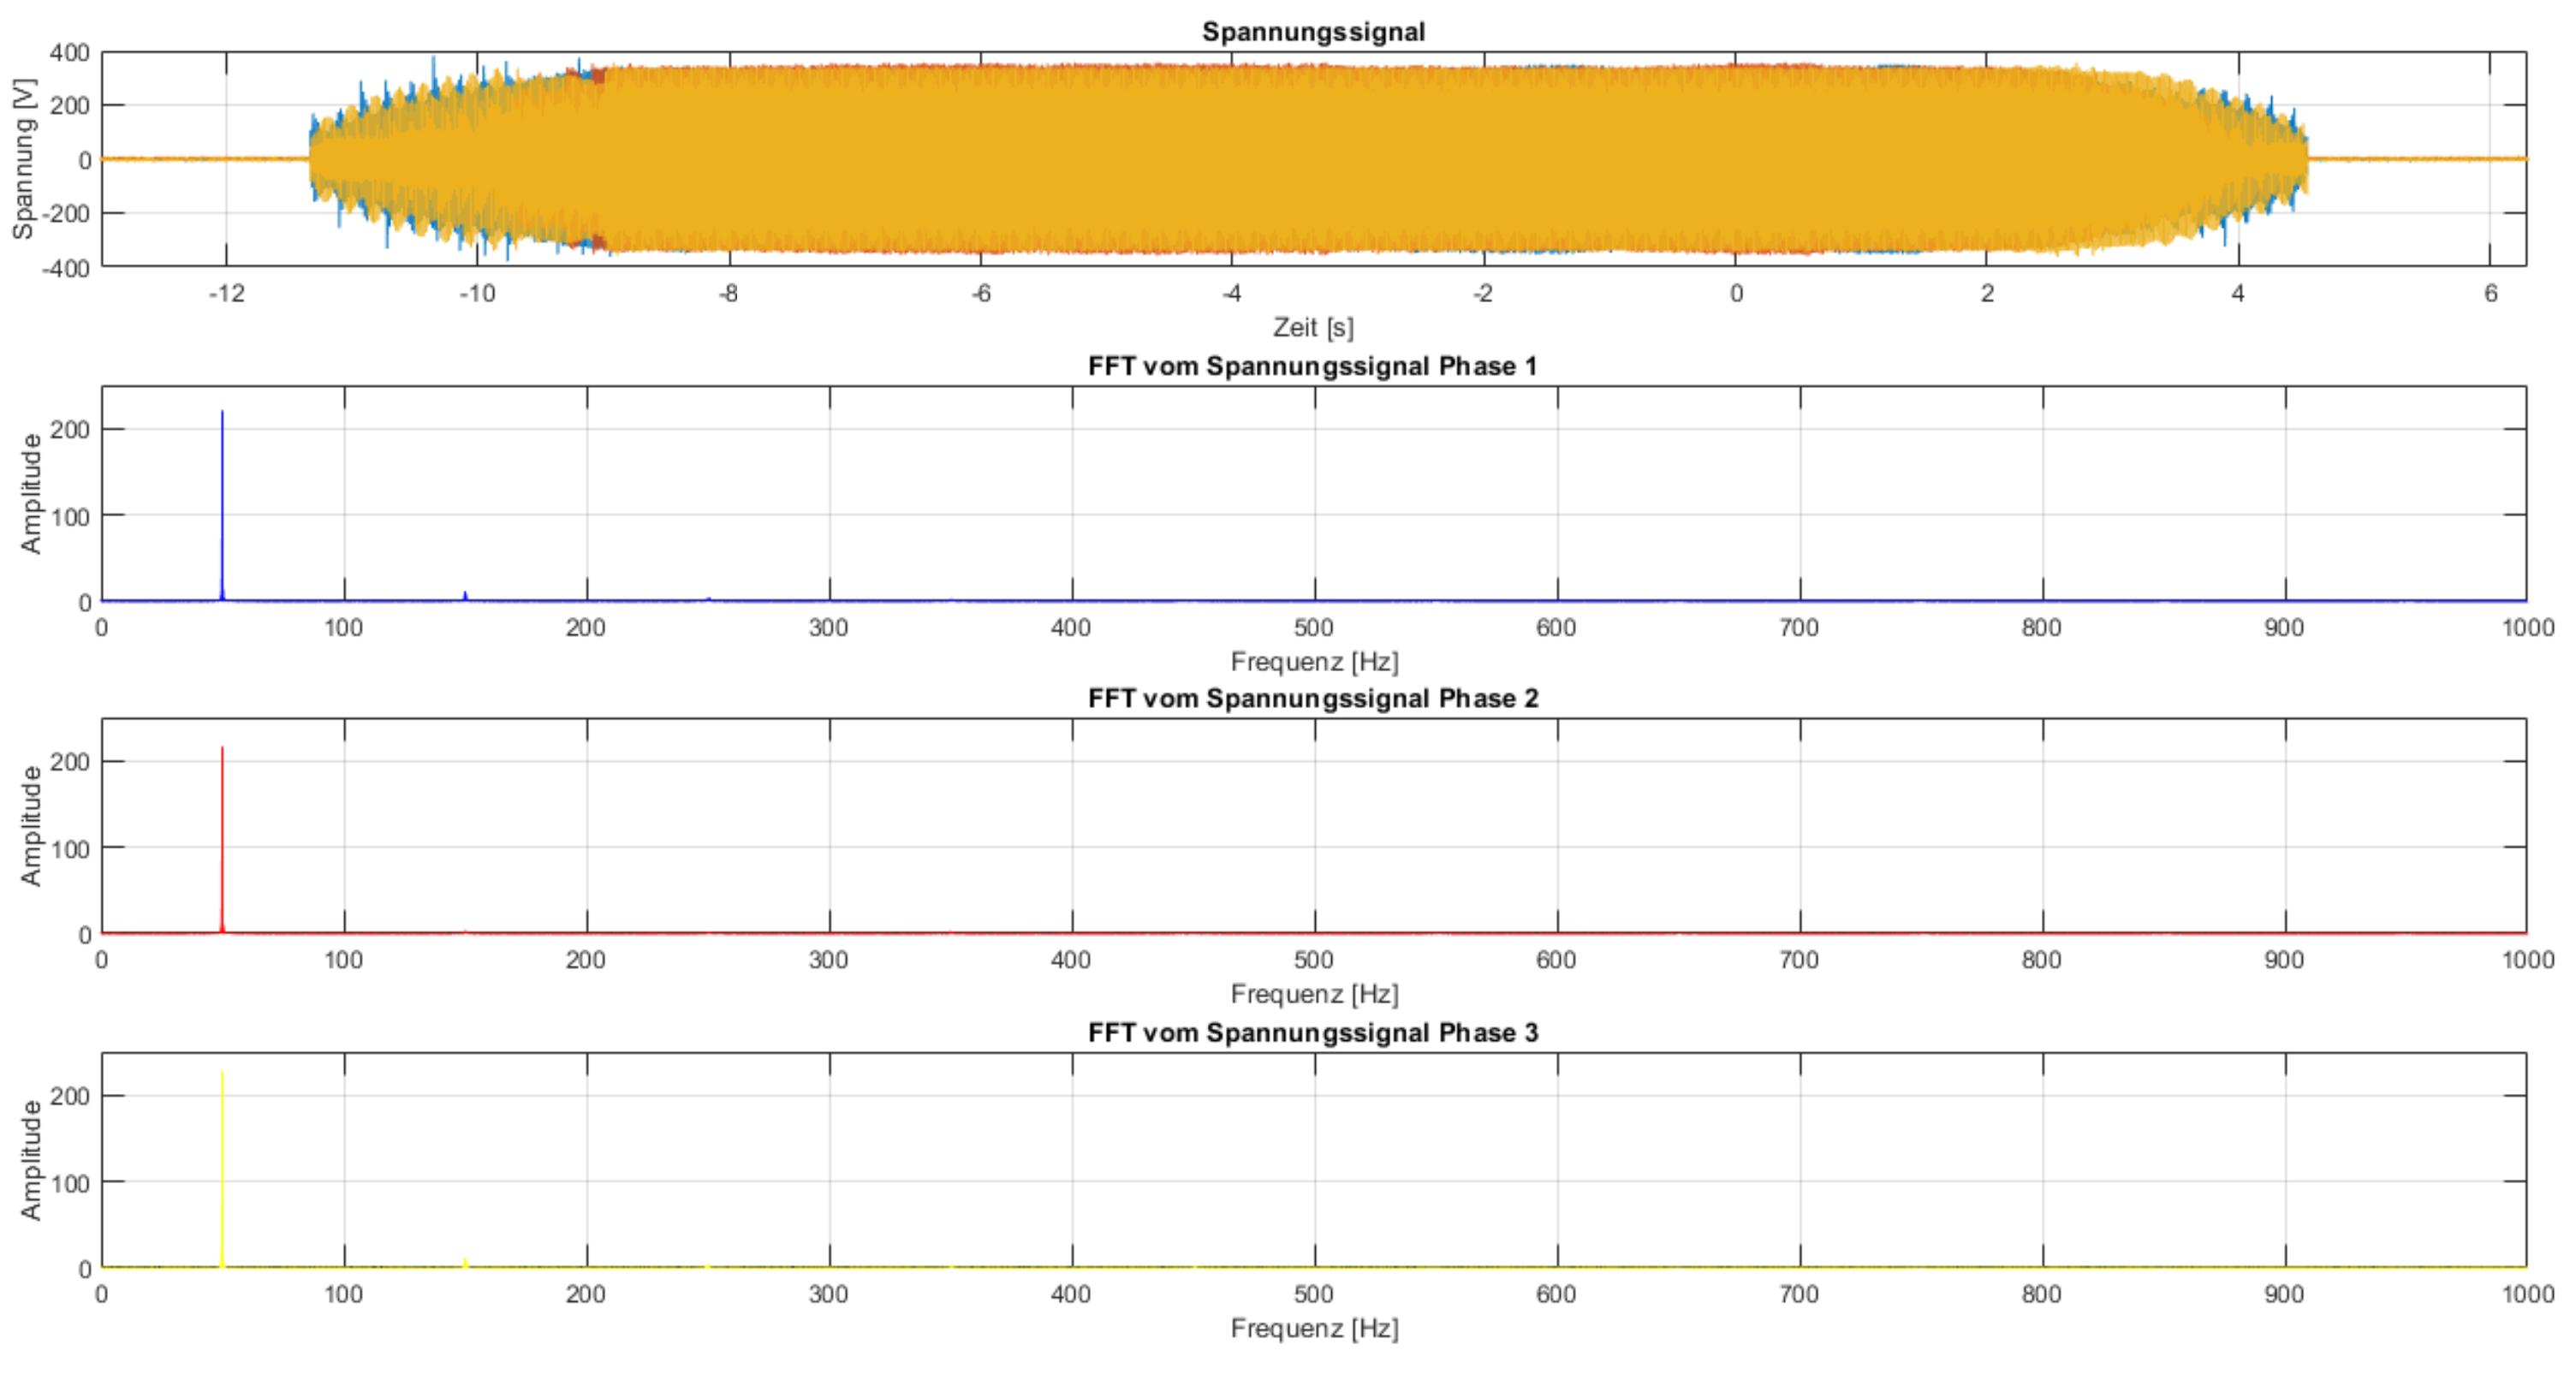
\includegraphics[width=0.96\textwidth]{Mess_ASM_2Thyristoren_AufAb_langsam.png}	
	\caption{Messung mit dem sanften Auf- und Absteuern und zwei Thyristoren}\label{fig:Mess_2Thyristoren_ASM_AufAbFahren_langsam}	
\end{figure}

\begin{table}[ht!]
	\centering
	\begin{tabular}{|l|l|l|l|}
		\hline
		Frequenz {[}Hz{]} & Amplitude Phase 1 {[}V{]}                                                           & Amplitude Phase 2 {[}V{]}                                                           & Amplitude Phase 3 {[}V{]}                                                           \\ \hline
		49.9              & 37.5857                                                                             & 42.9618                                                                             & 47.1945                                                                             \\ \hline
		49.95             & 75.5033                                                                             & 87.0174                                                                             & 77.0178                                                                             \\ \hline
		50                & 220.7586                                                                            & 216.2571                                                                            & 227.9957                                                                            \\ \hline
		50.05             & 111.631                                                                             & 110.0439                                                                            & 102.3768                                                                            \\ \hline
		50.1              & 44.4045                                                                             & 65.6359                                                                             & 40.8044                                                                             \\ \hline
		149.95            & 6.9369                                                                              & 2.1636                                                                              & 5.8686                                                                              \\ \hline
		150               & 11.5575                                                                             & 1.4866                                                                              & 10.115                                                                              \\ \hline
		150.05            & 6.7811                                                                              & 2.7637                                                                              & 6.5154                                                                              \\ \hline \hline
		Frequenz {[}Hz{]} & \begin{tabular}[c]{@{}l@{}}Verhältnis zur \\ Grundschwingung\\ Phase 1\end{tabular} & \begin{tabular}[c]{@{}l@{}}Verhältnis zur \\ Grundschwingung\\ Phase 2\end{tabular} & \begin{tabular}[c]{@{}l@{}}Verhältnis zur \\ Grundschwingung\\ Phase 3\end{tabular} \\ \hline
		49.9              & 17.03\%                                                                             & 19.46\%                                                                             & 20.7\%                                                                              \\ \hline
		49.95             & 34.2\%                                                                              & 39.42\%                                                                             & 33.78\%                                                                             \\ \hline
		50                & 100\%                                                                               & 100\%                                                                               & 100\%                                                                               \\ \hline
		50.05             & 50.57\%                                                                             & 49.85\%                                                                             & 44.9\%                                                                              \\ \hline
		50.1              & 20.11\%                                                                             & 29.73\%                                                                             & 17.9\%                                                                              \\ \hline
		149.95            & 3.16\%                                                                              & 0.98\%                                                                              & 2.57\%                                                                              \\ \hline
		150               & 5.24\%                                                                              & 0.67\%                                                                              & 4.44\%                                                                              \\ \hline
		150.05            & 3.07\%                                                                              & 1.25\%                                                                              & 2.86\%                                                                              \\ \hline
	\end{tabular}
	\caption{Amplitudenwerte bei der Frequenzen mit zwei Thyristoren bei sanftem Auf- und Absteuern}\label{tab:Mess_2Thyristoren_Spannung_ASM_AufAb_sanft}
\end{table}

\newpage
\subsection{Sparvariante für den Widerstand mit einem Thyristor} \label{sec:Sparvariante_1Thyristor}
\subsubsection*{Phasenanschnitt 60\textdegree}

\begin{figure}[ht]
	\centering
	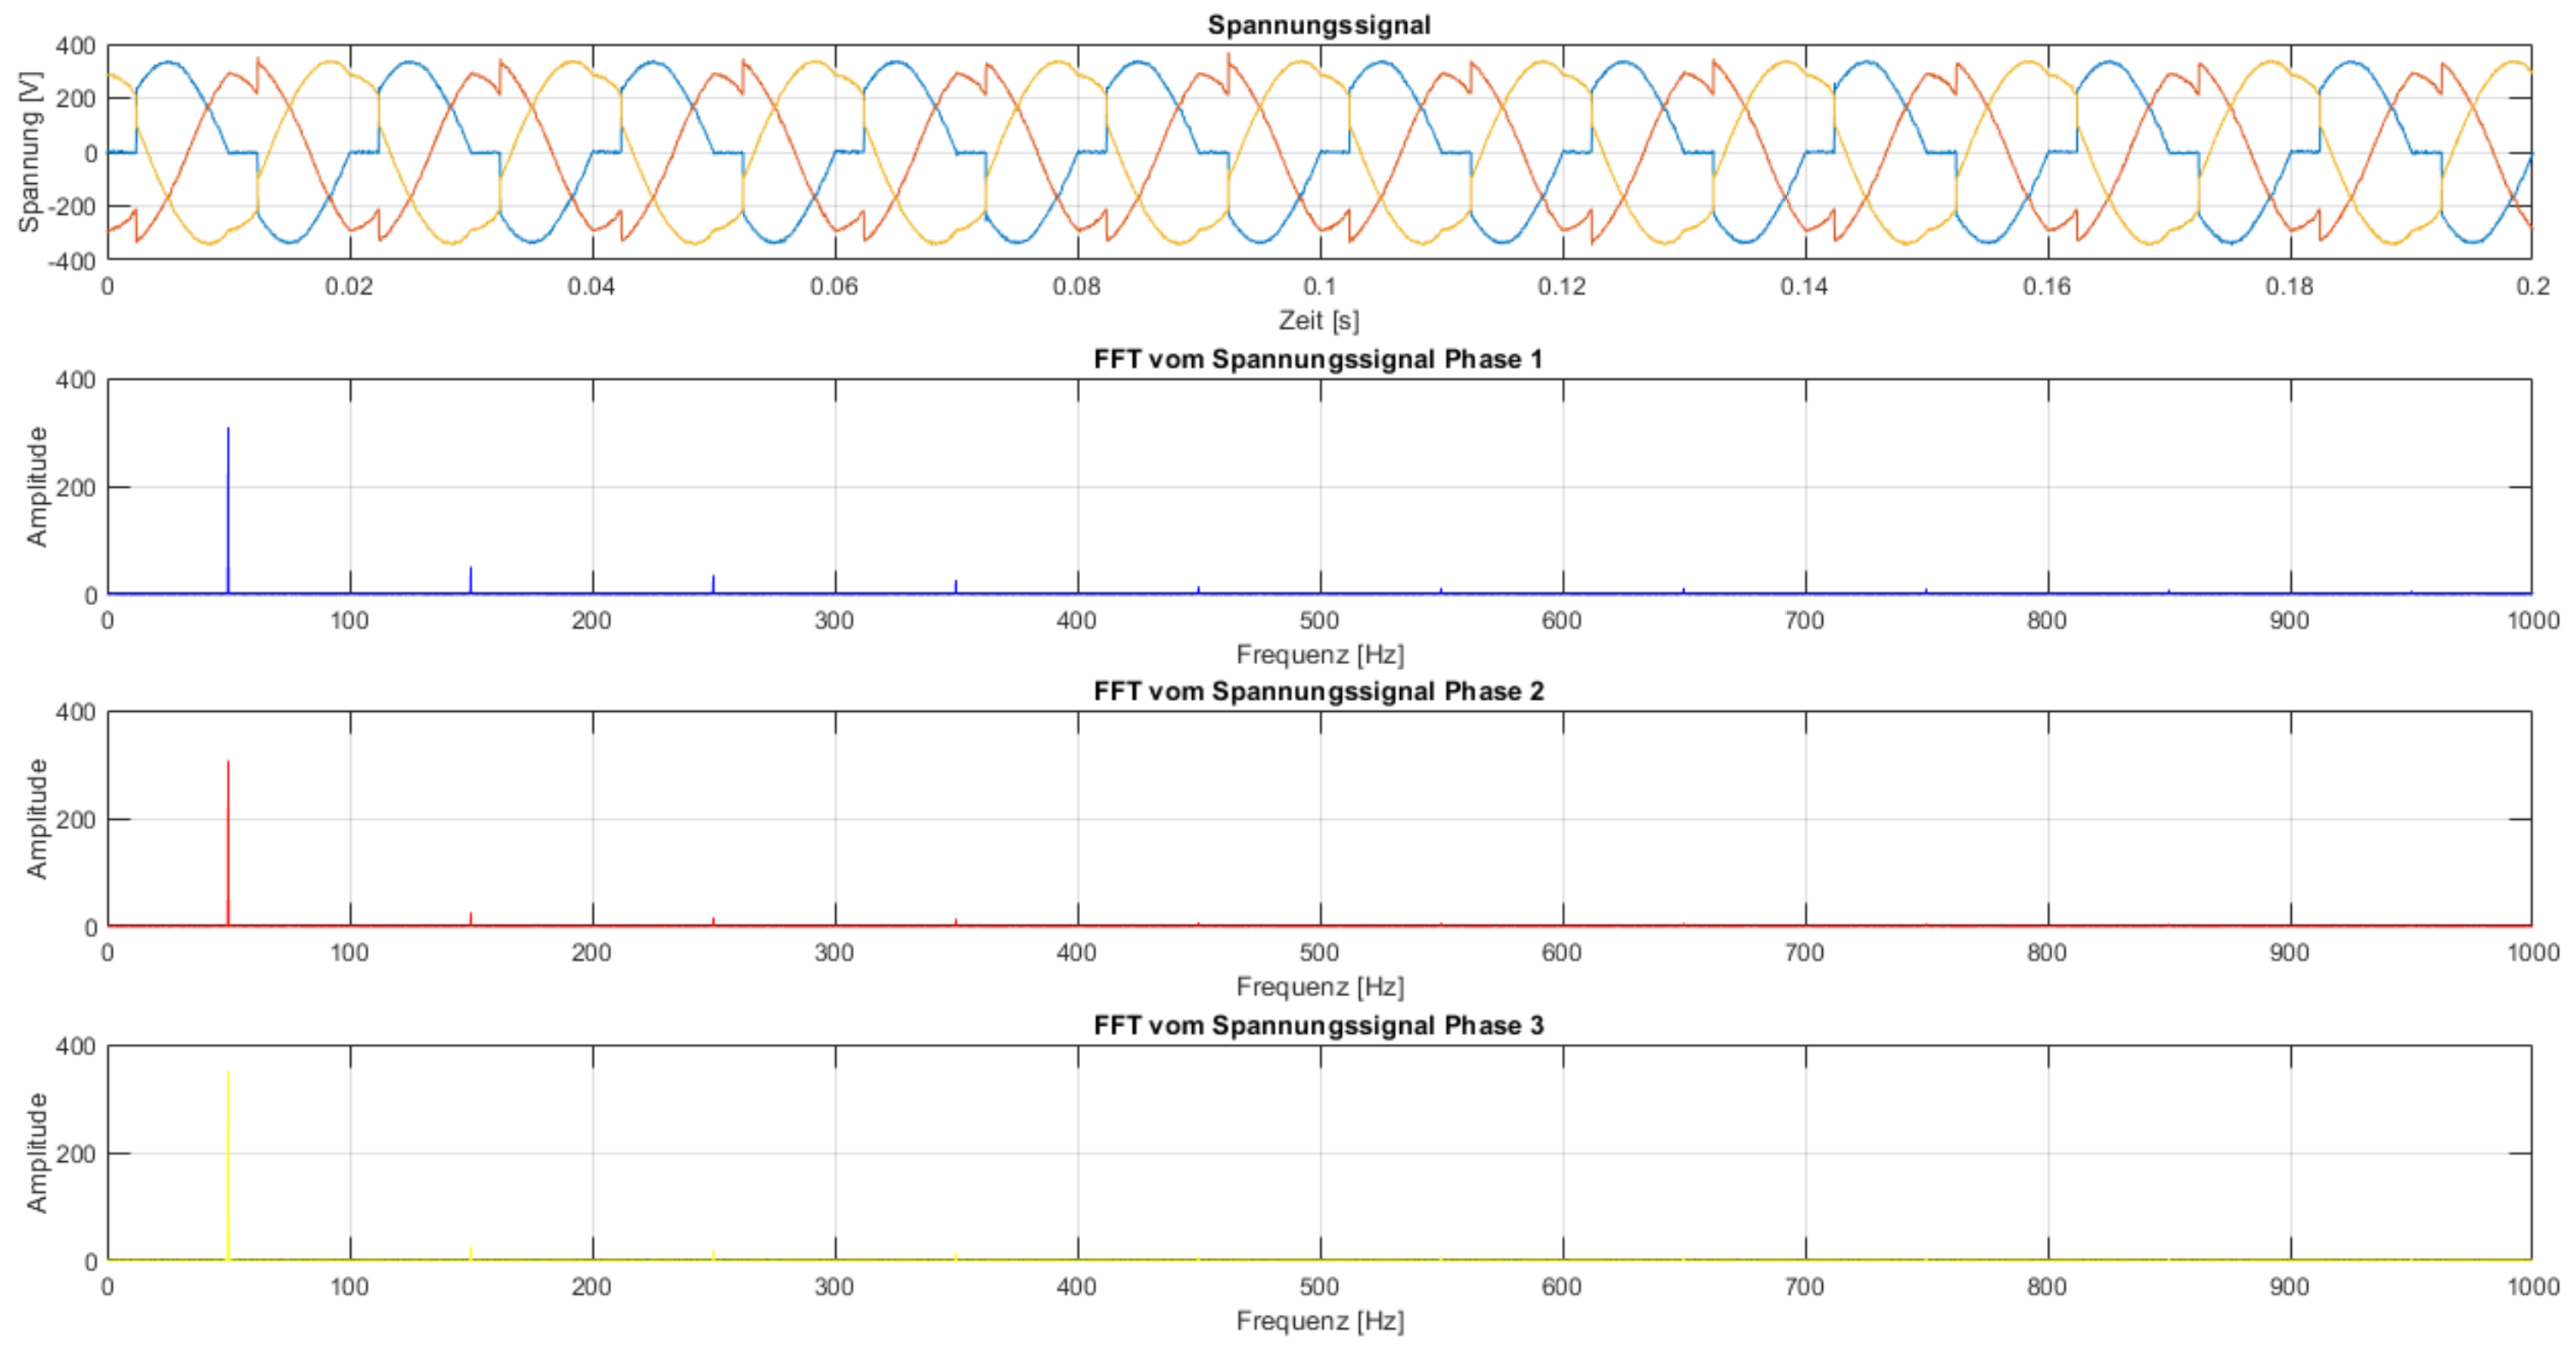
\includegraphics[width=0.96\textwidth]{Mess_1Thyristor_Widerstand_Phas60.png}	
	\caption{Messung mit Phasenanschnitt 60\textdegree \hspace{0.02cm} und einem Thyristoren}\label{fig:Mess_1Thyristor_Phas_60grad}
\end{figure}


\subsubsection*{Phasenanschnitt 90\textdegree}

\begin{figure}[ht]
	\centering
	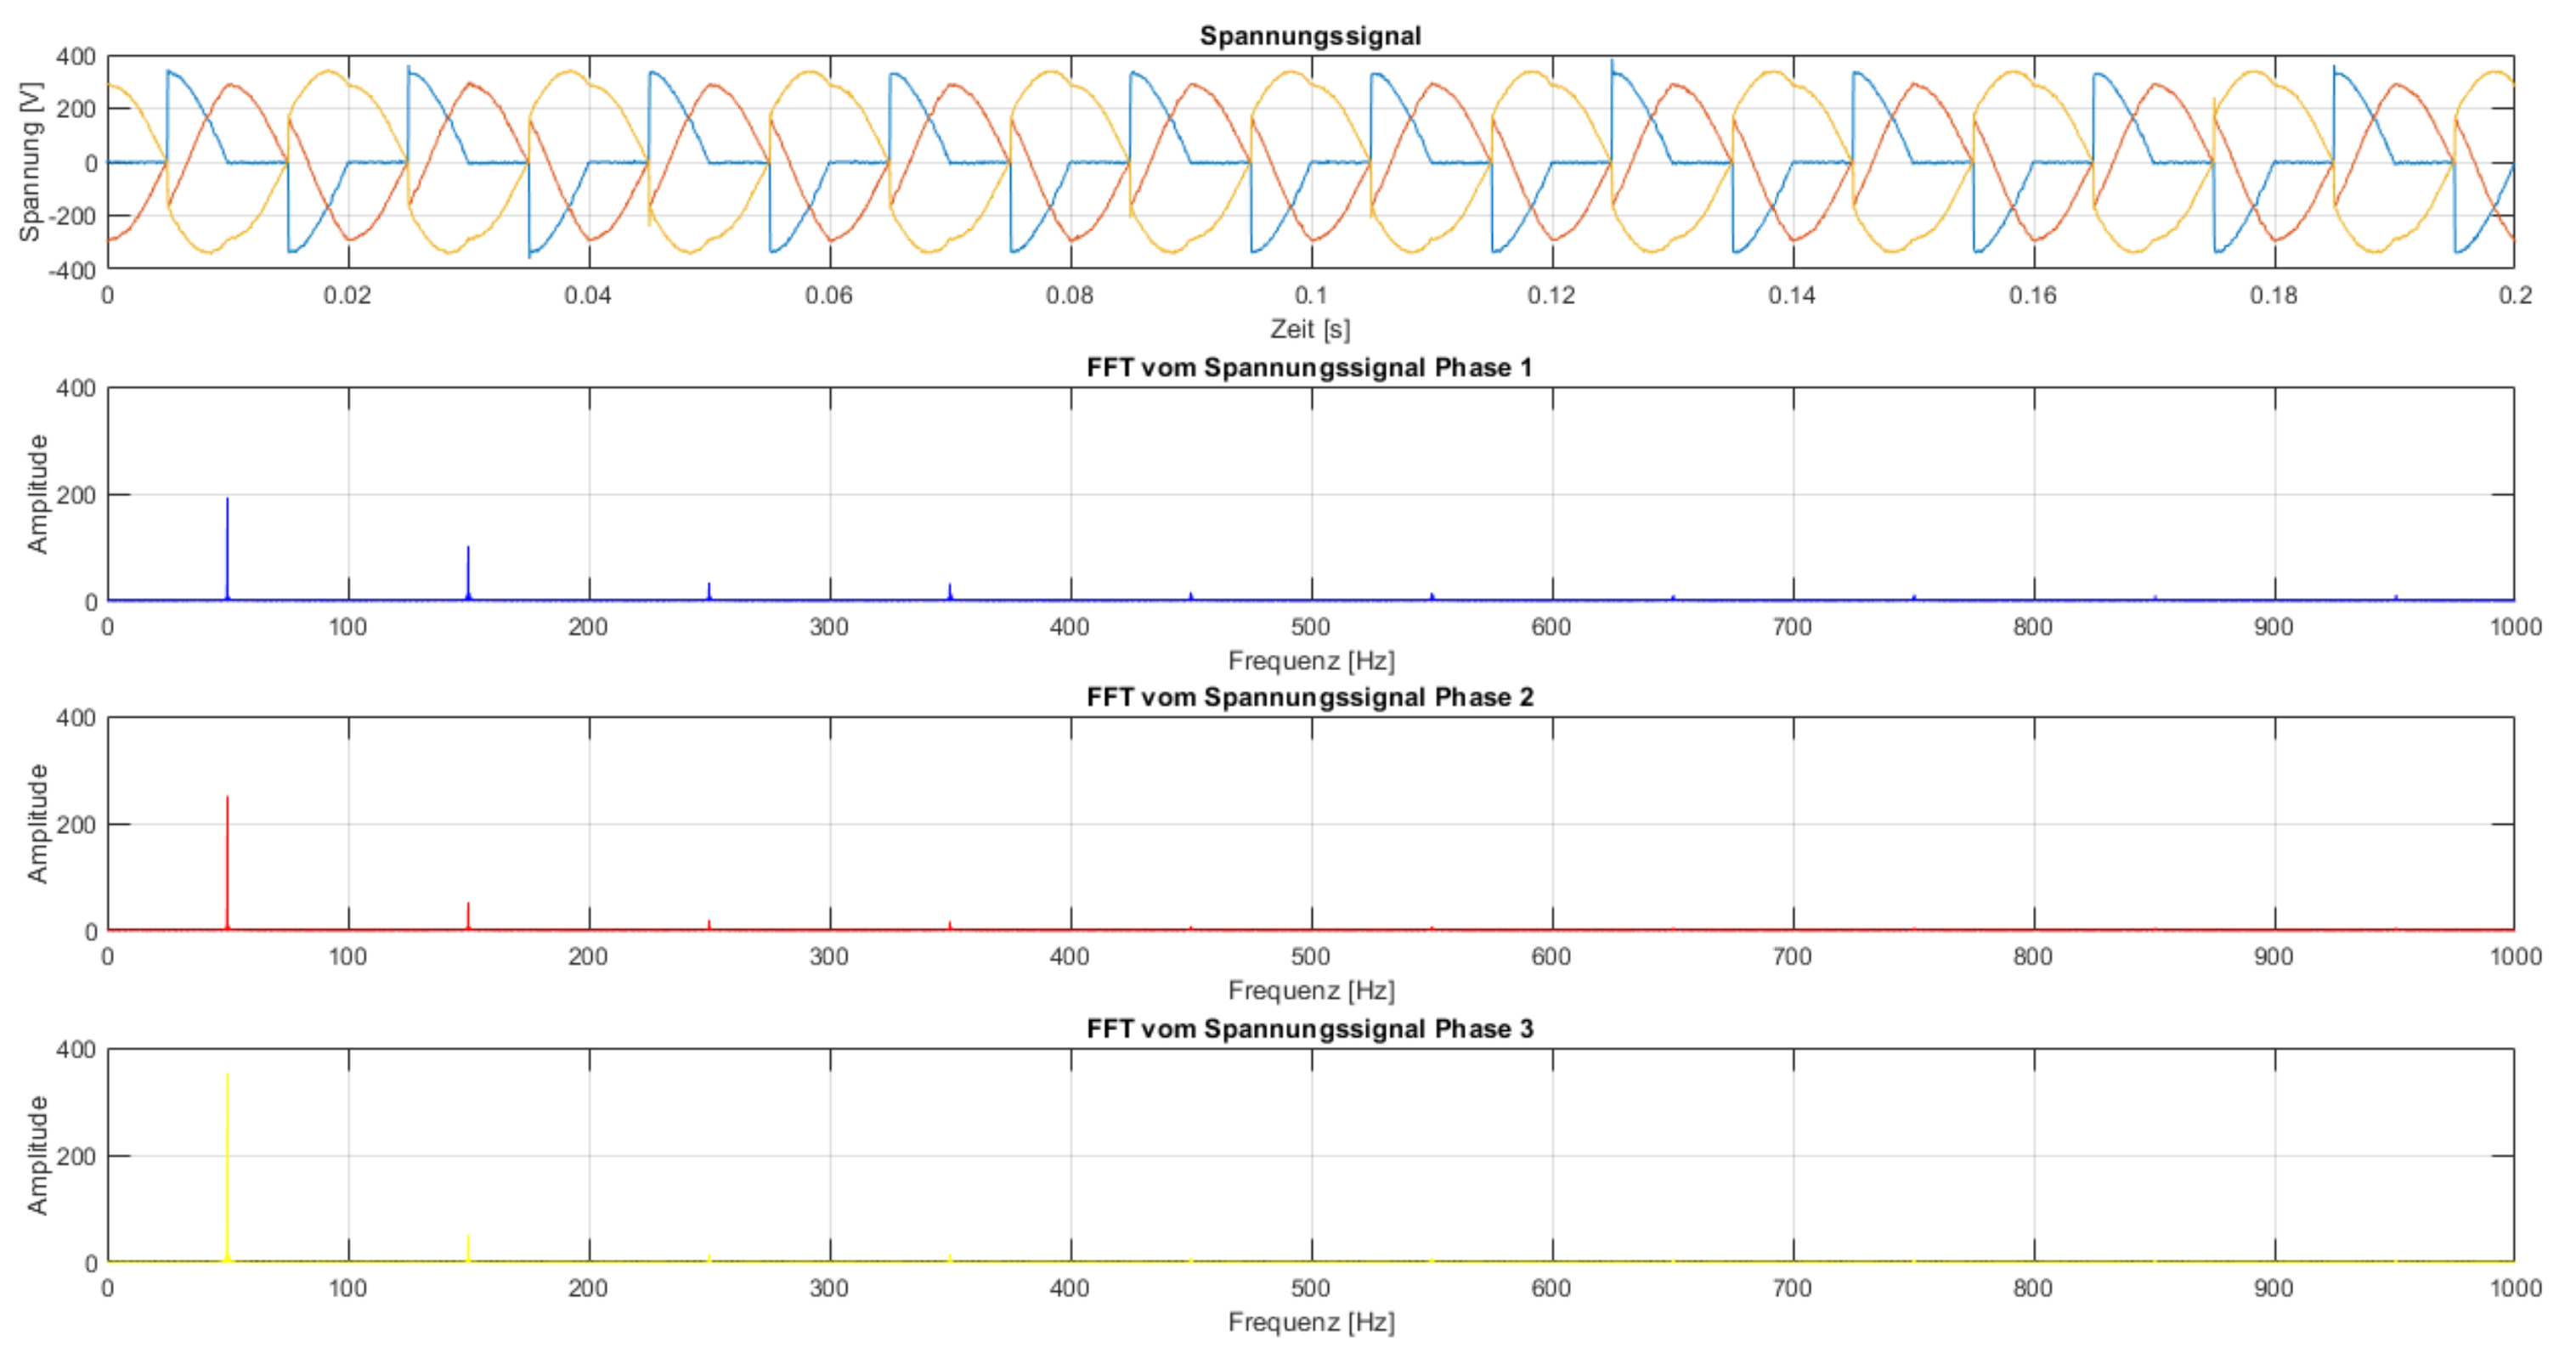
\includegraphics[width=0.96\textwidth]{Mess_1Thyristor_Widerstand_Phas90.png}	
	\caption{Messung mit Phasenanschnitt 90\textdegree \hspace{0.02cm} und einem Thyristoren}\label{fig:Mess_1Thyristor_Phas_90grad}
\end{figure}

\newpage
\subsubsection*{Schwingungspaket mit einem Duty Cycle von 0.5}

\begin{figure}[ht]
	\centering
	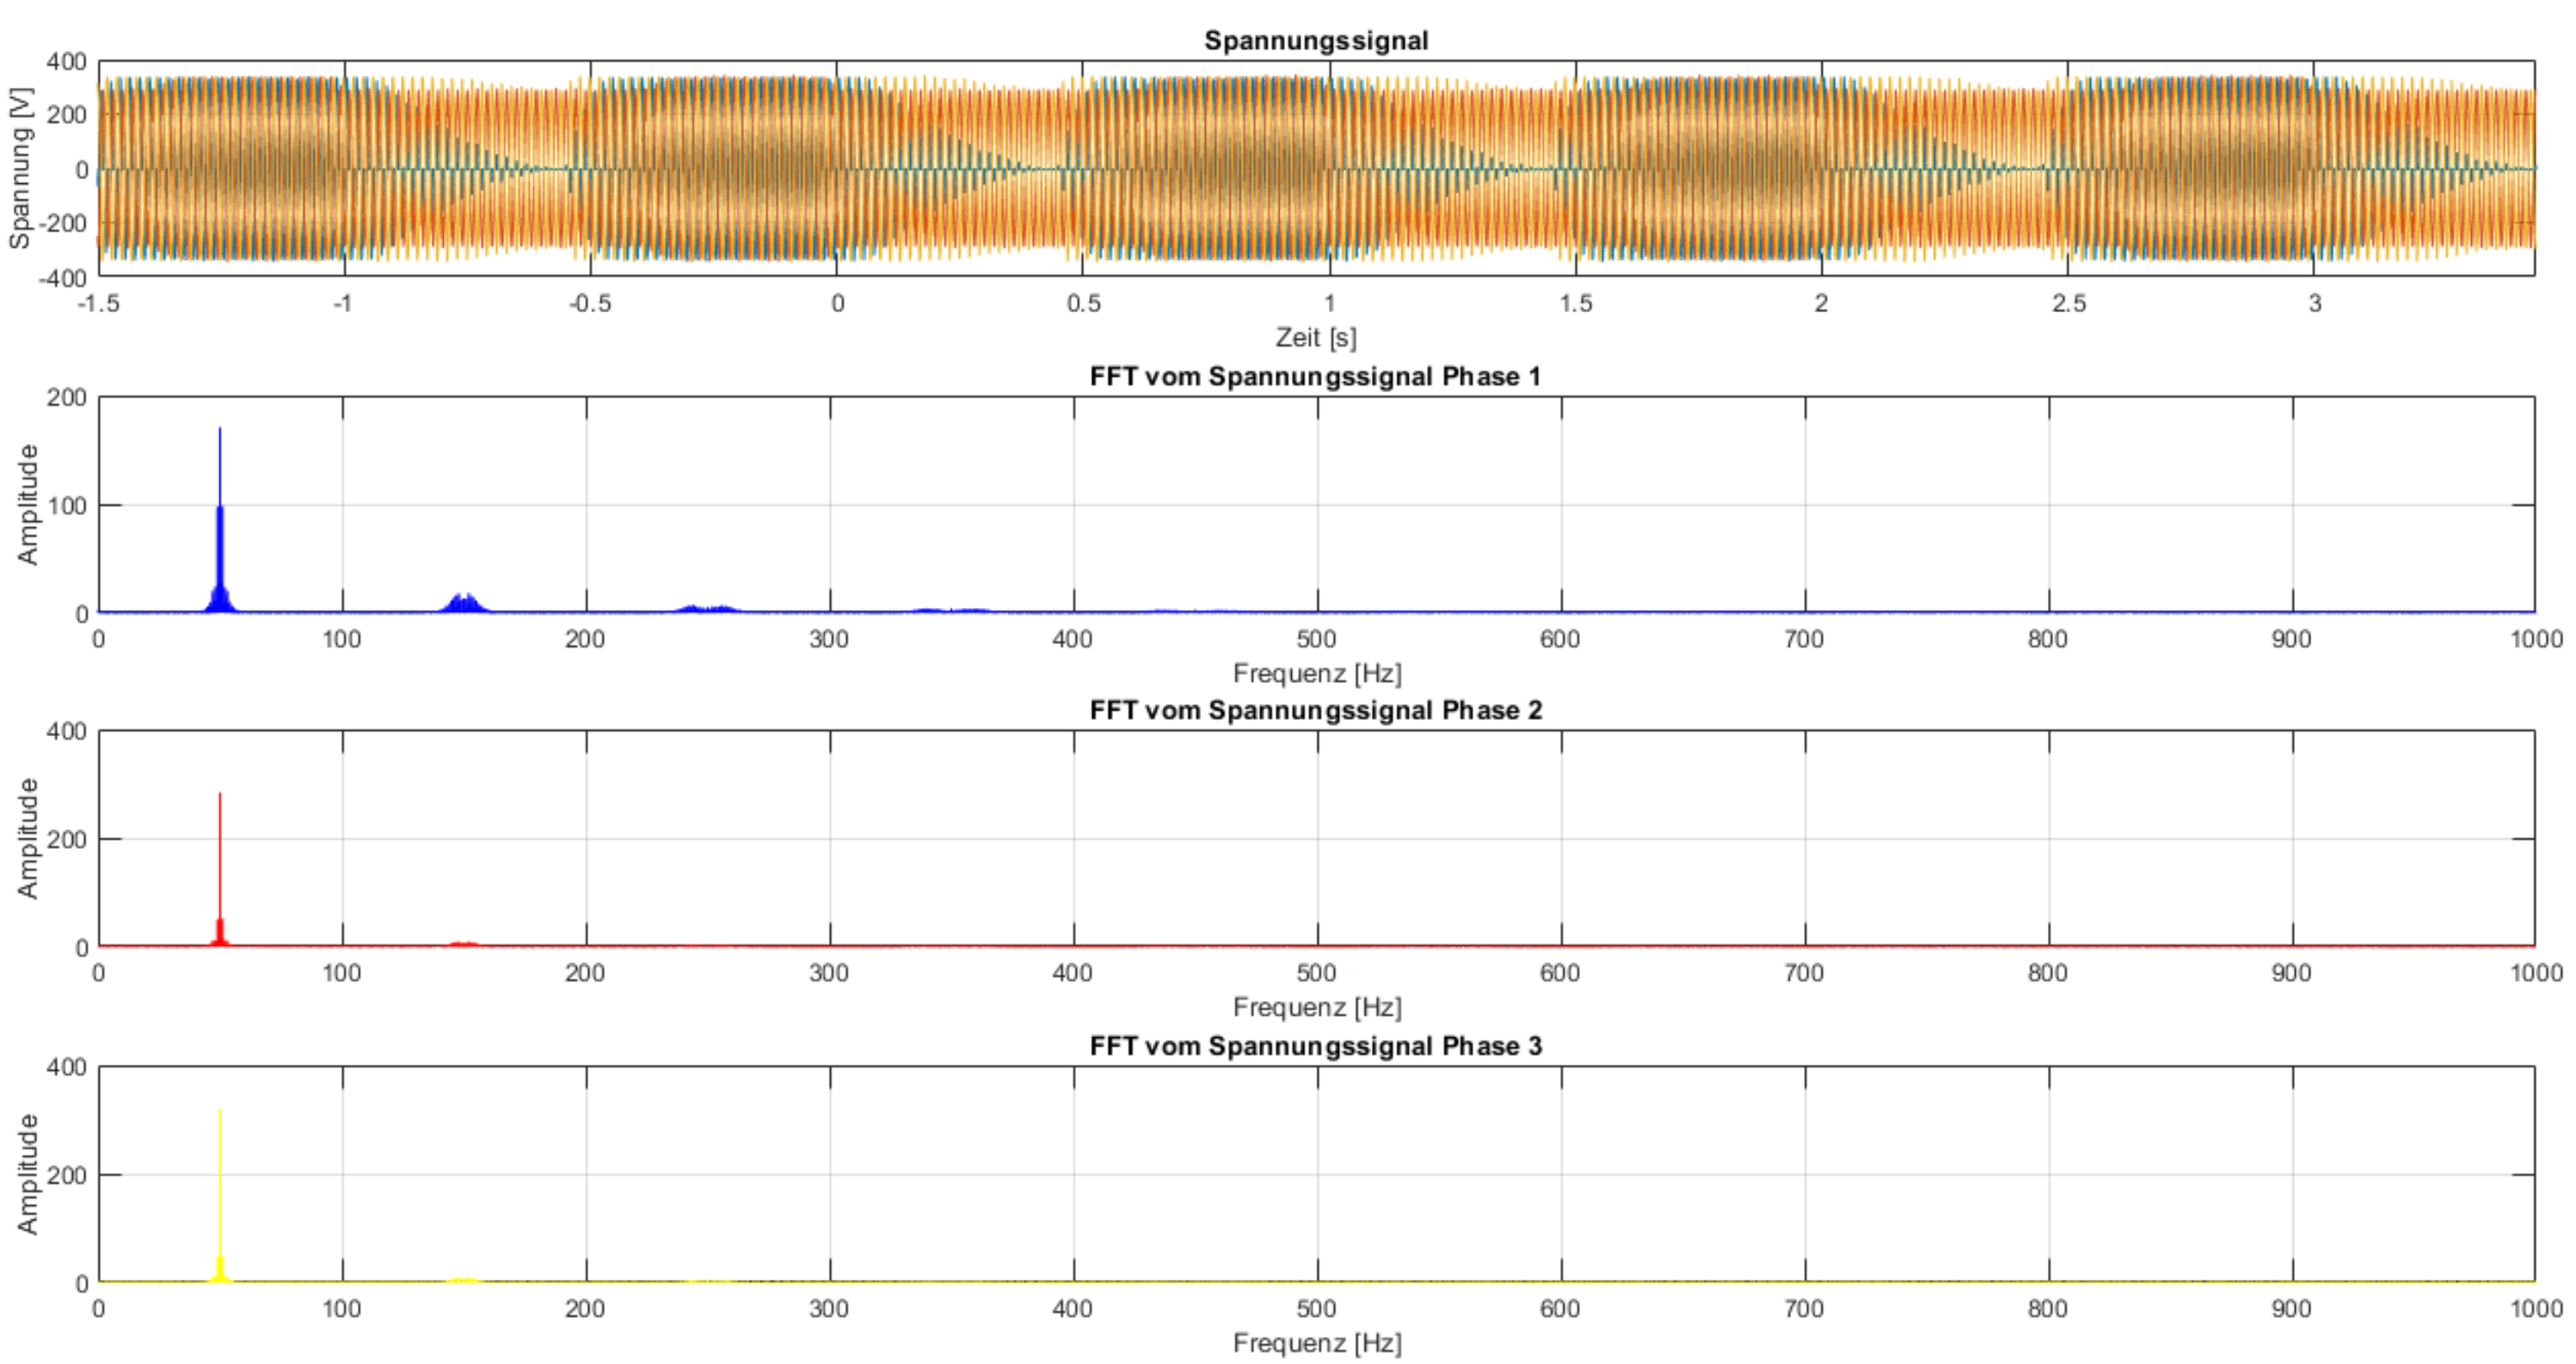
\includegraphics[width=0.9\textwidth]{Mess_1Thyristor_Widerstand_Schwing_05.png}	
	\caption{Messung mit Schwingungspaket mit einem Duty Cycle von 0.5 und einem Thyristoren}\label{fig:Mess_1Thyristor_Schwing_50}
\end{figure}

\subsubsection*{Schwingungspaket mit einem Duty Cycle von 0.8}

\begin{figure}[ht]
	\centering
	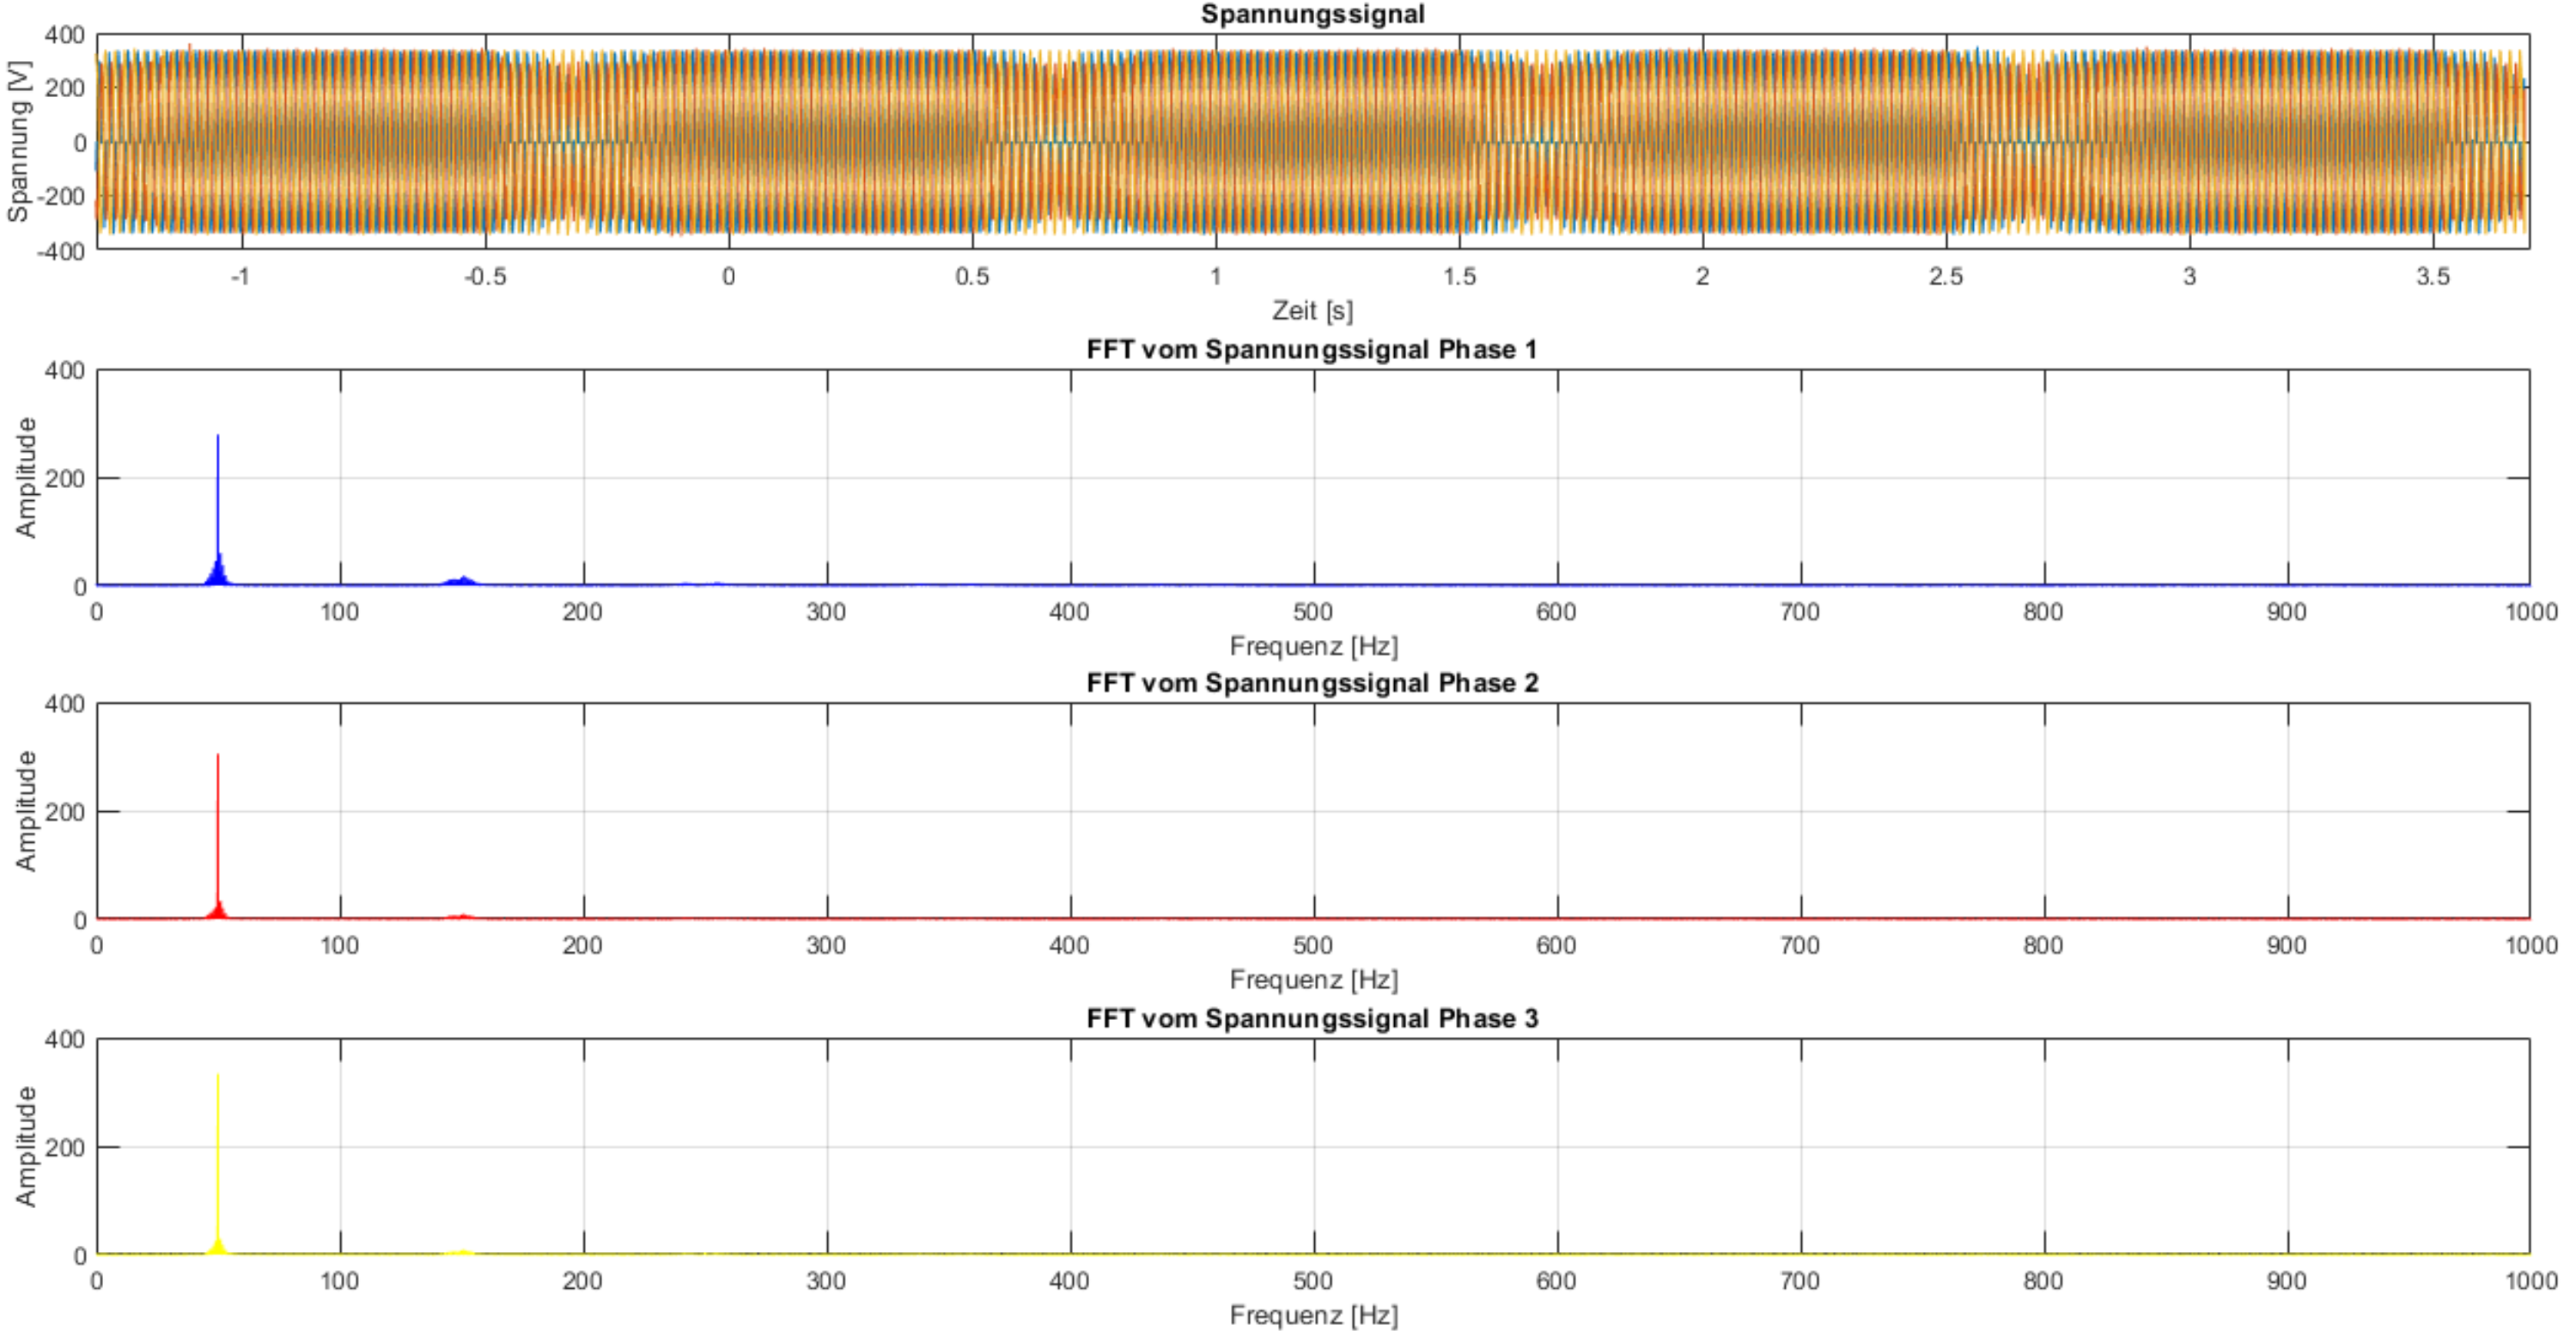
\includegraphics[width=0.9\textwidth]{Mess_1Thyristor_Widerstand_Schwing_08.png}	
	\caption{Messung mit Schwingungspaket mit einem Duty Cycle von 0.8 und einem Thyristoren}\label{fig:Mess_1Thyristoren_Schwing_80}	
\end{figure}

\newpage
\subsubsection*{Auf- und Absteuern}

\begin{figure}[ht]
	\centering
	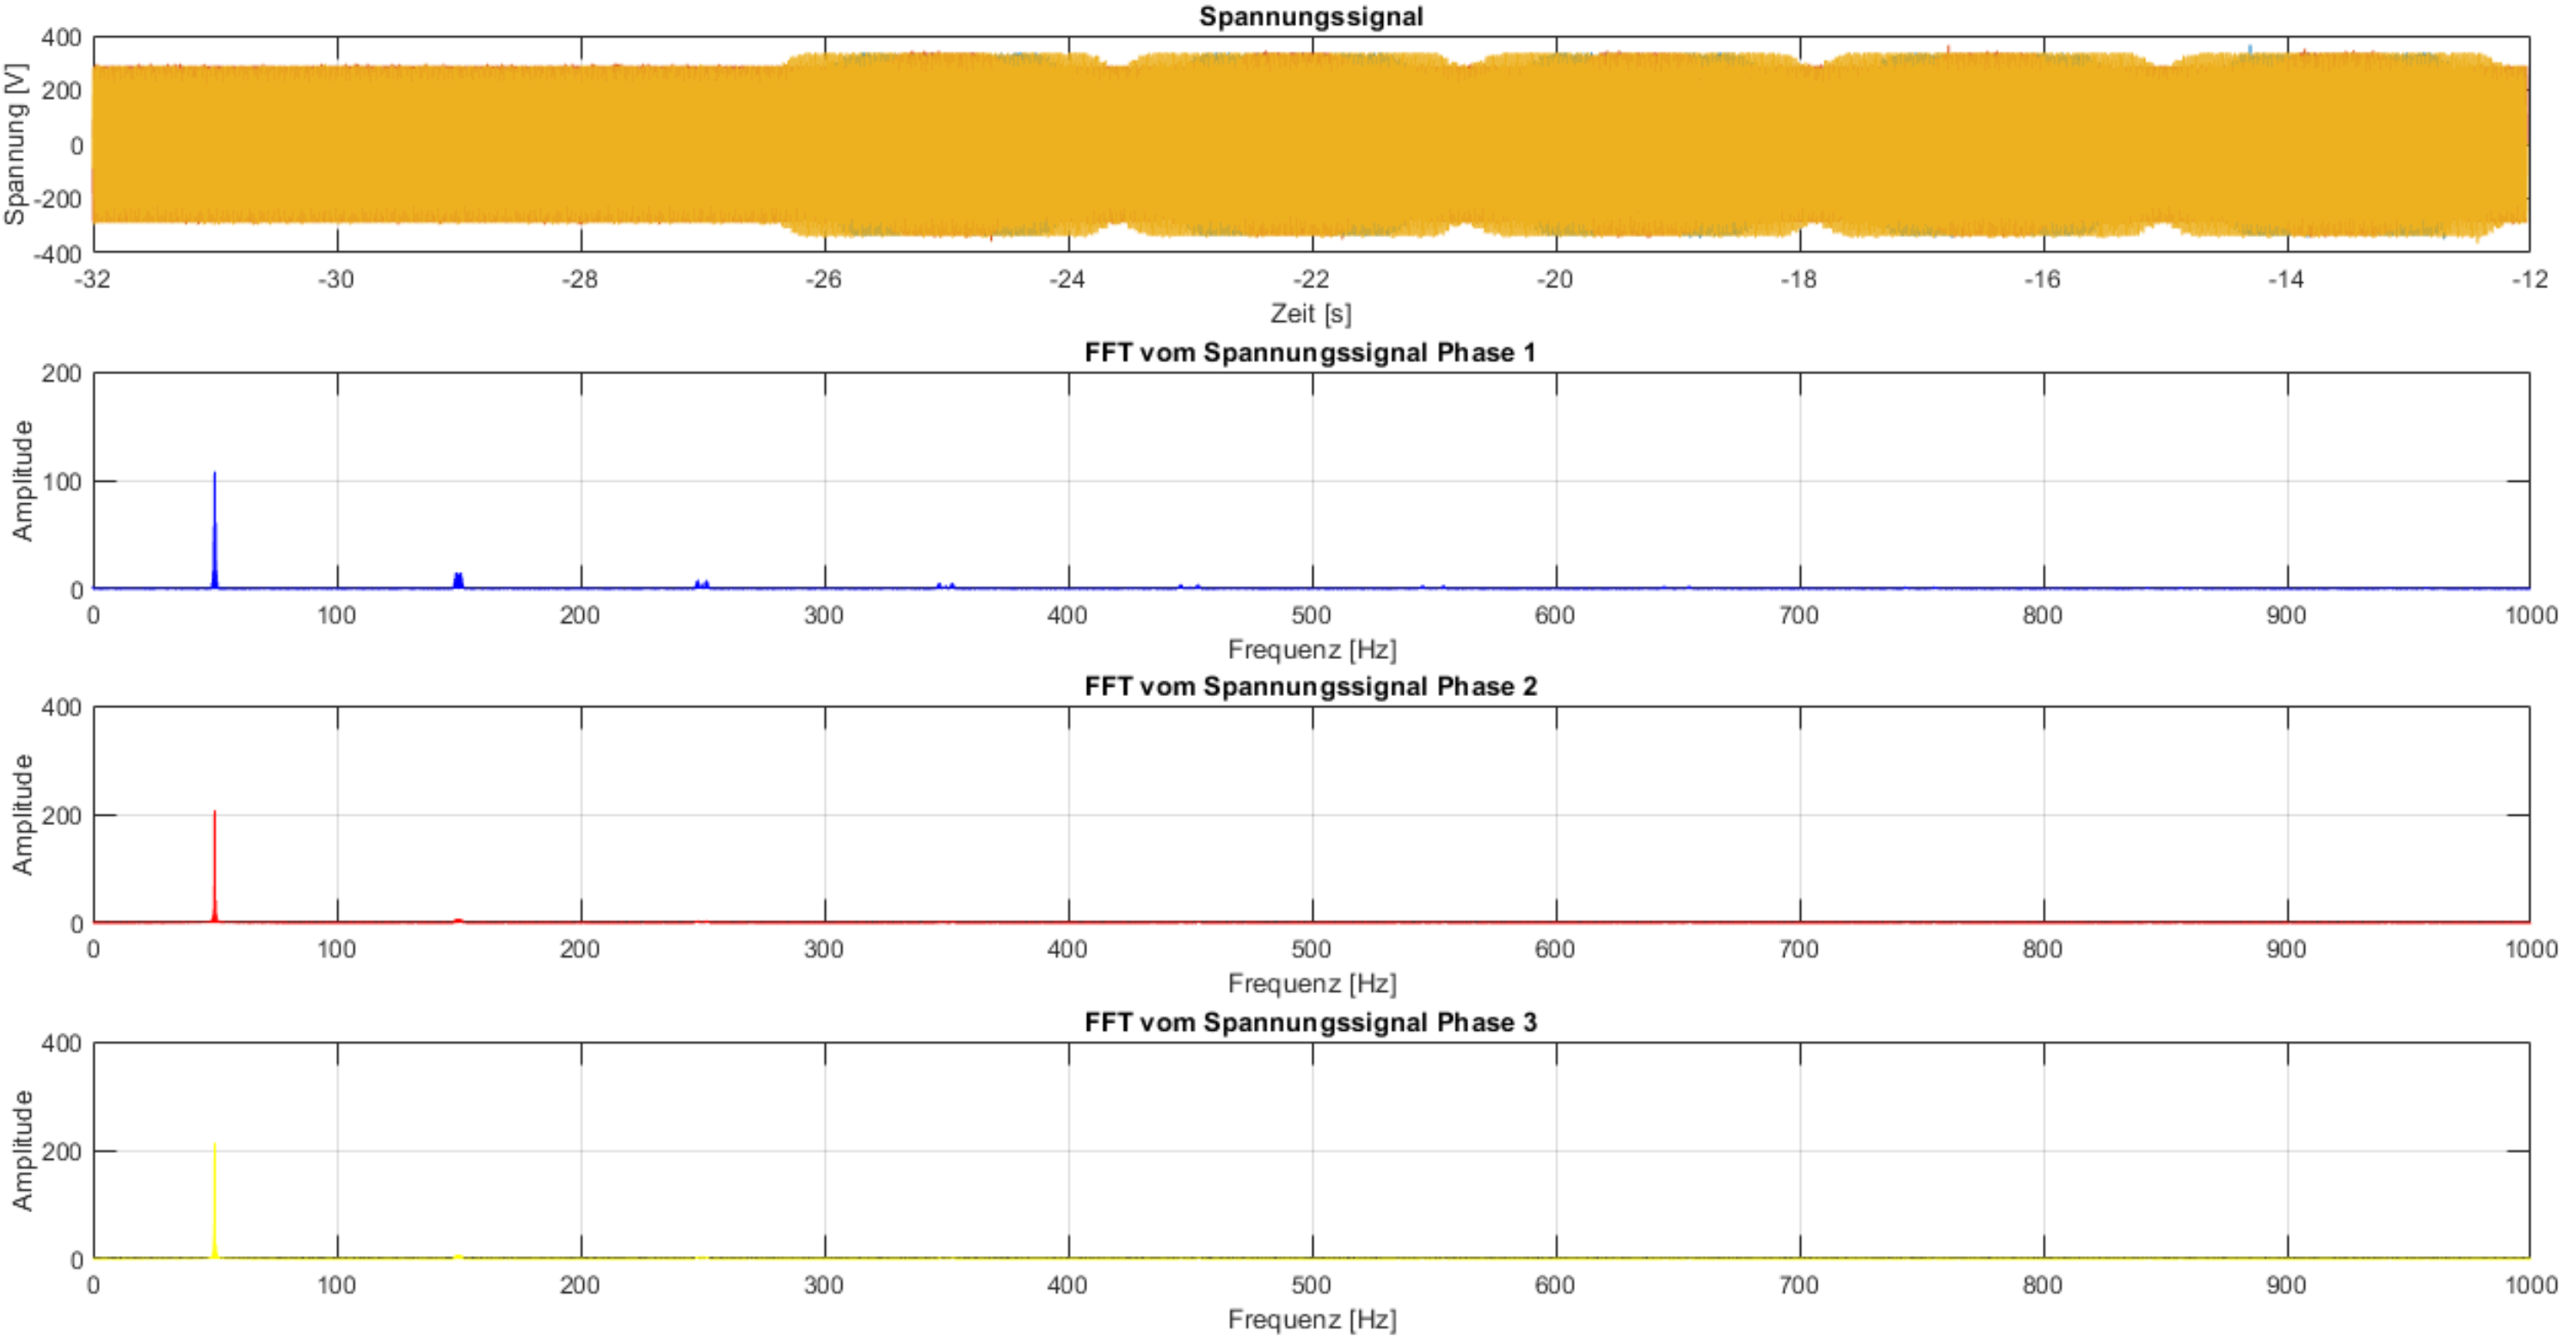
\includegraphics[width=0.9\textwidth]{Mess_1Thyristor_Widerstand_AufAb.png}	
	\caption{Messung mit Auf- und Absteuern und einem Thyristoren}\label{Mess_1Thyristoren_Widerstand_AufAbFahren}	
\end{figure}


\subsubsection*{Langsames Auf- und Absteuern}

\begin{figure}[ht]
	\centering
	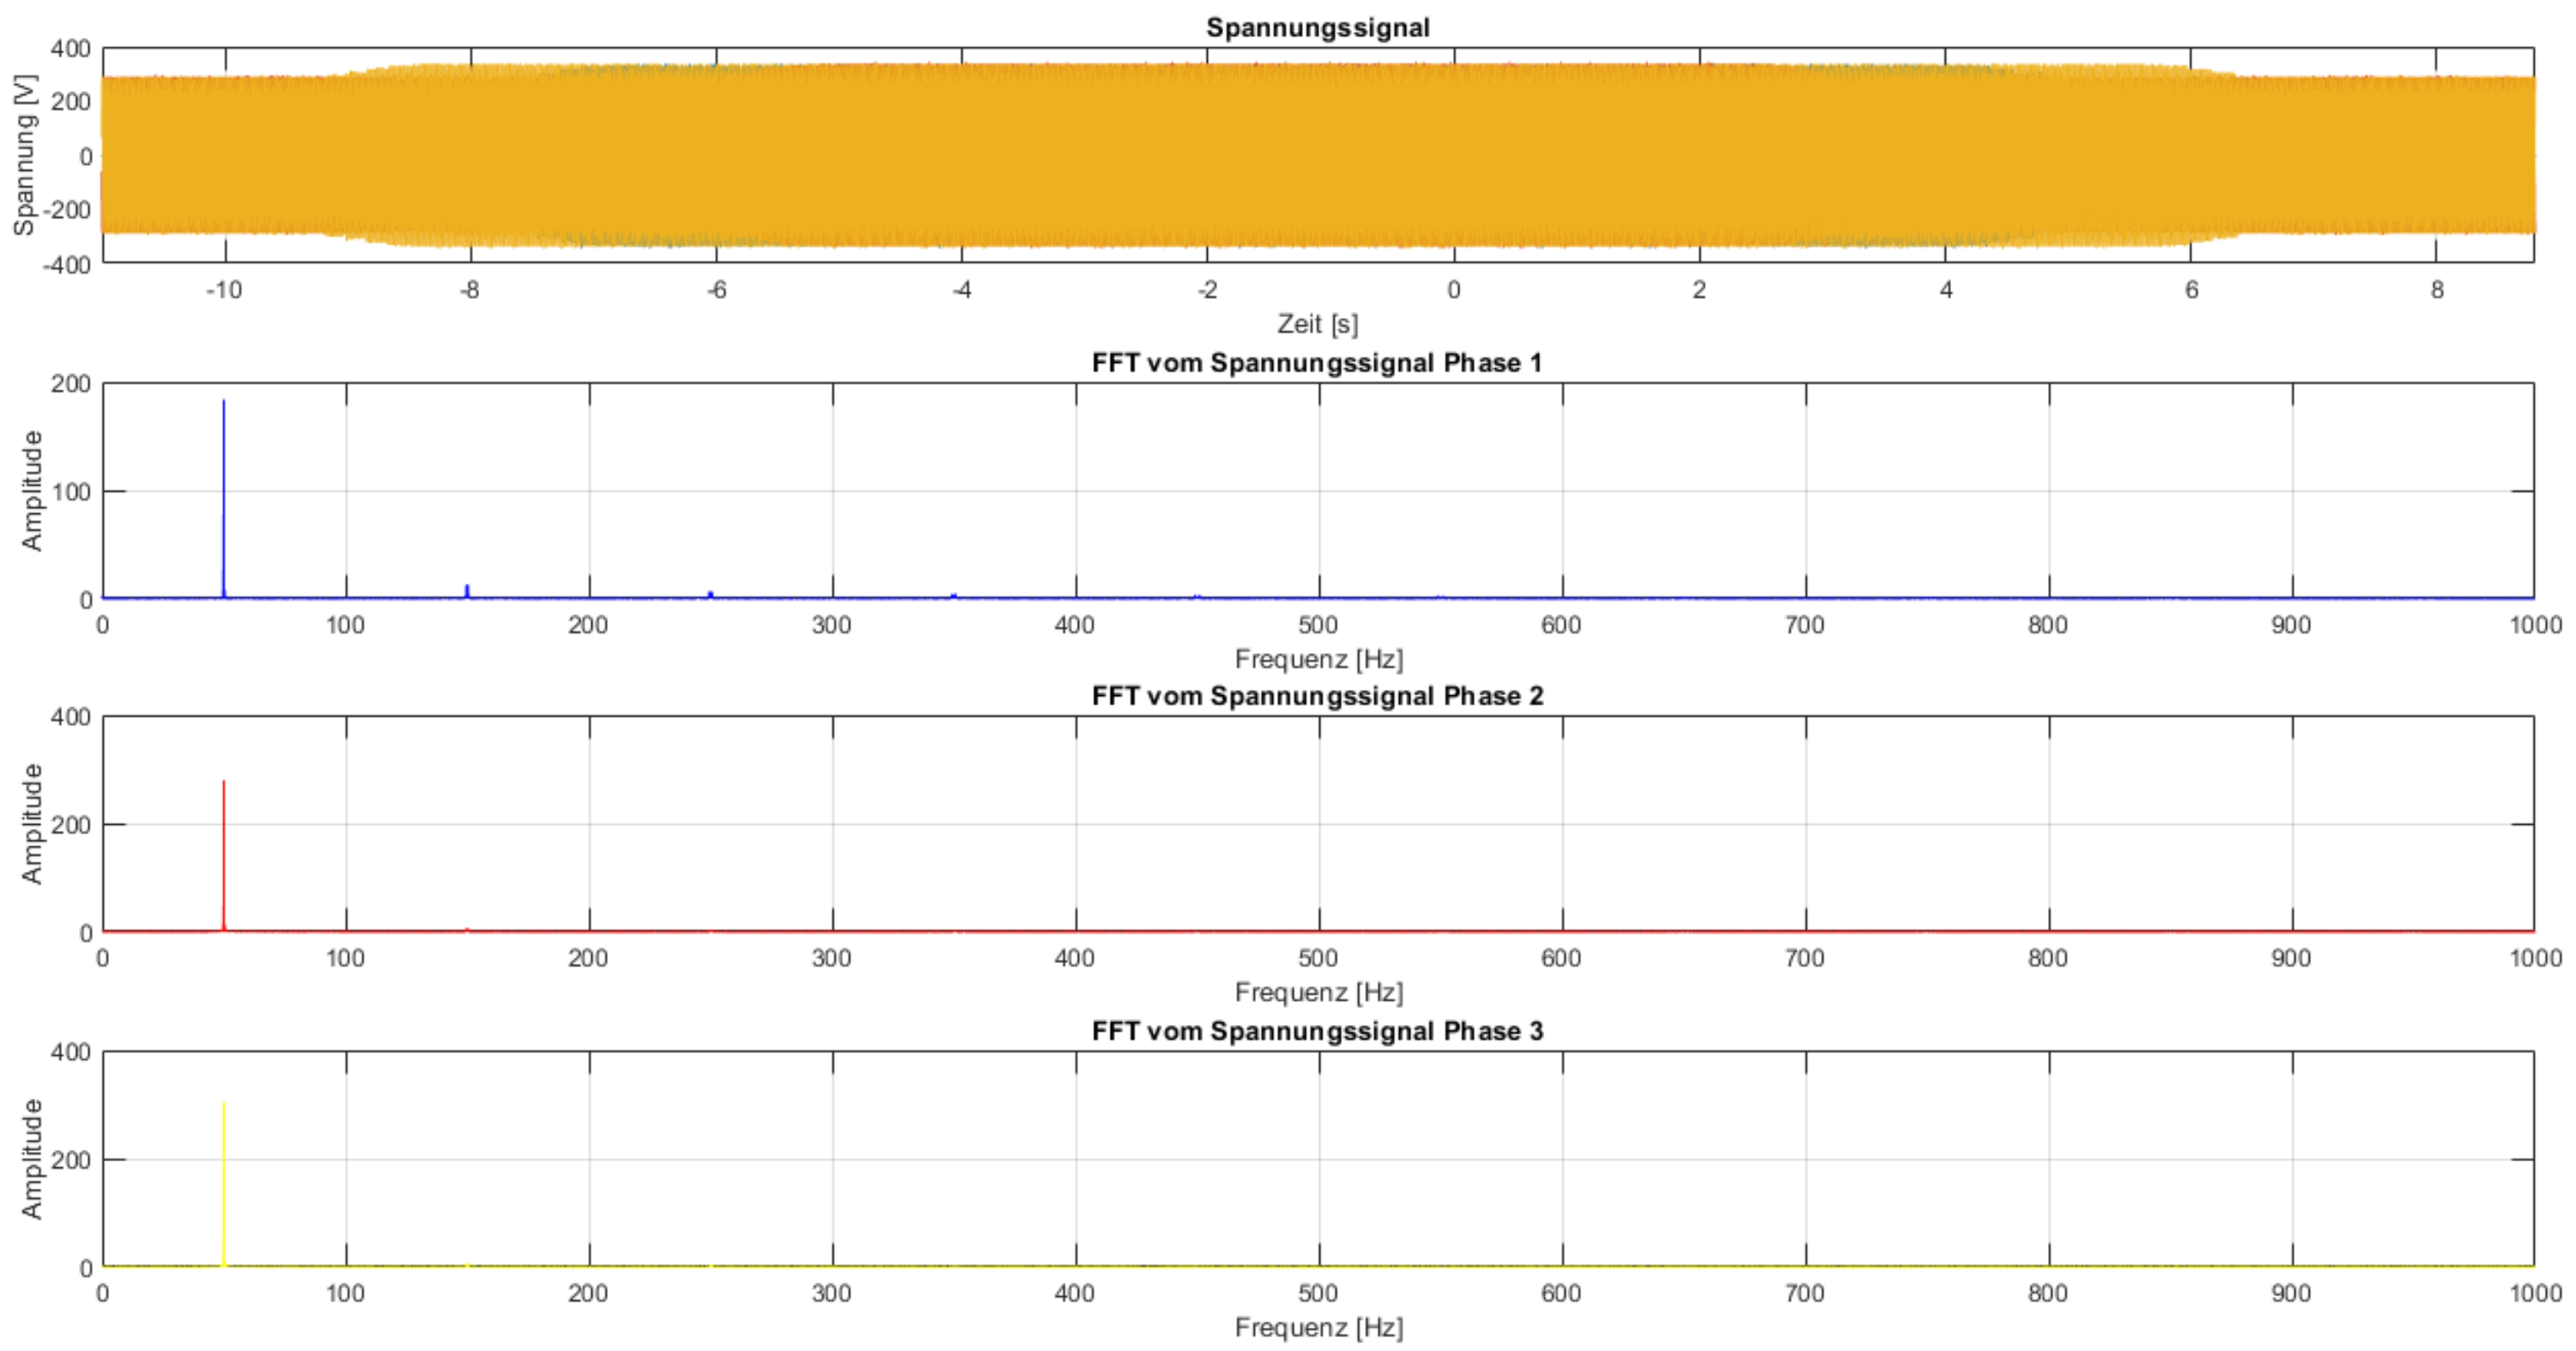
\includegraphics[width=0.9\textwidth]{Mess_1Thyristor_Widerstand_AufAb_langsam.png}	
	\caption{Messung mit dem langsamen Auf- und Absteuern und einem Thyristoren}\label{Mess_1Thyristoren_Widerstand_AufAbFahren_langsam}	
\end{figure}

\newpage
\subsection{Vergleich Messungen Widerstand mit Simulation}
\subsubsection*{Schwingungspaket mit einem Duty Cycle von 0.5} \label{sec:Vergleich_Mess_Sim_Schwing_50}

\begin{figure}[ht!]
	\begin{minipage}[b]{0.59\textwidth}
		\centering
		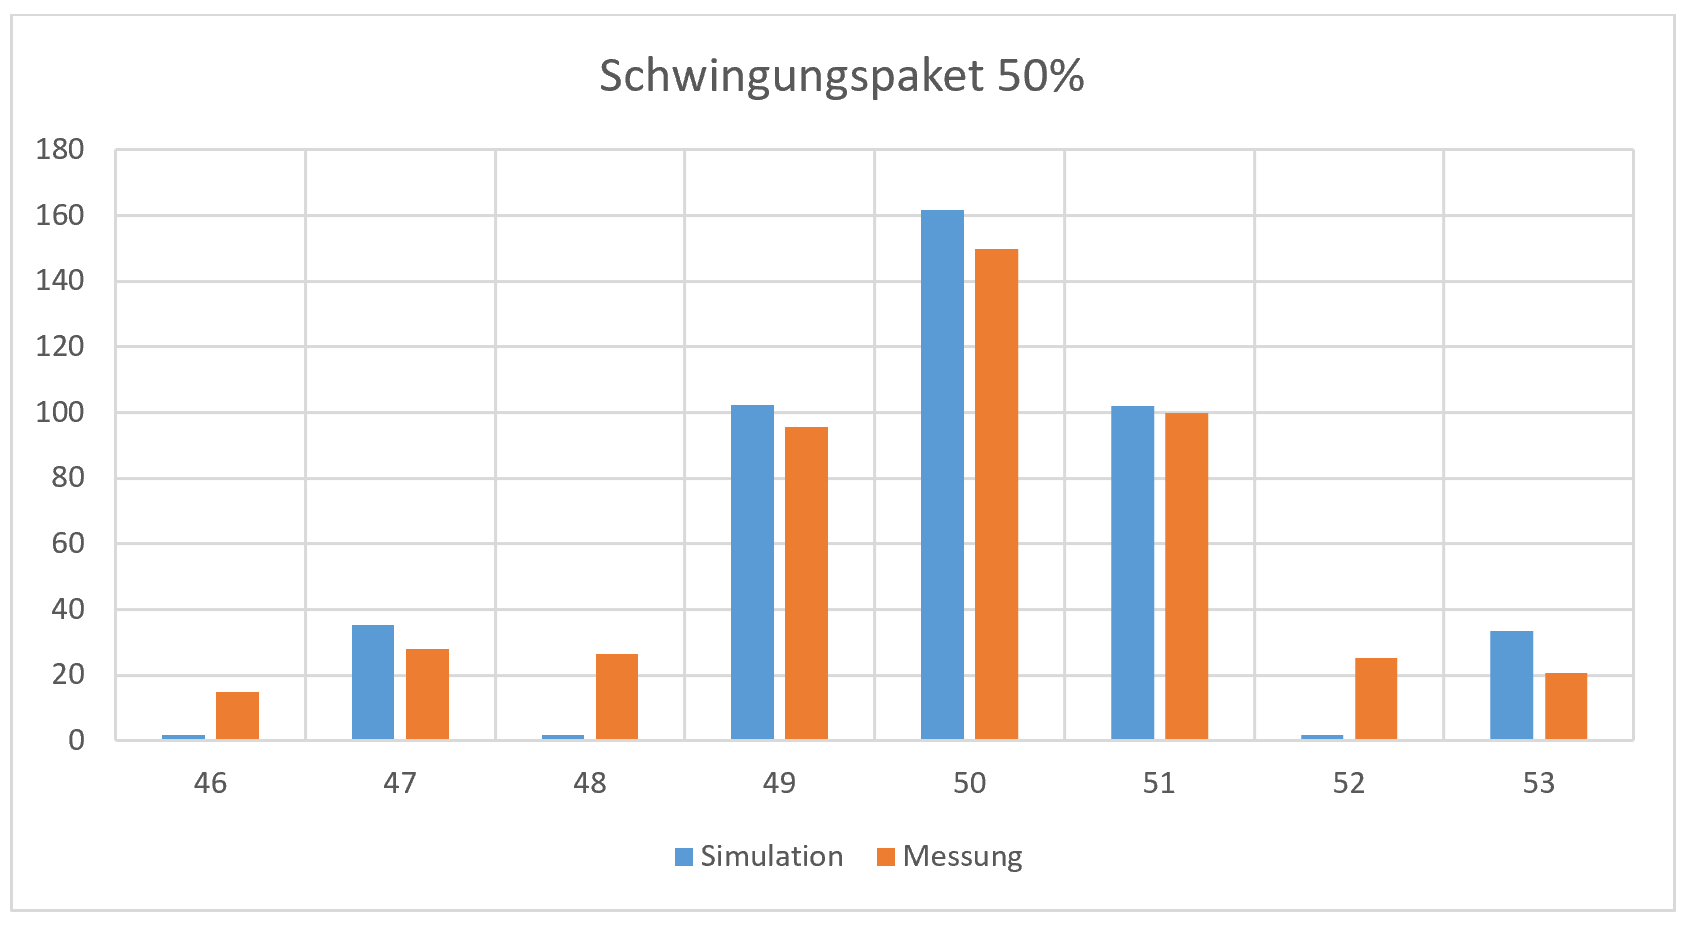
\includegraphics[width=\textwidth]{Vergleich_Mess_Sim_Schwing_50.png}	
		\caption{Vergleich Messung und Simulation mit Schwingungspaket mit einem Duty Cycle von 0.5}\label{fig:Vergleich_Schwing_50}
	\end{minipage}
	%
	\begin{minipage}[b]{0.4\textwidth}
		\centering
		\begin{tabular}{|l|l|l|}
			\hline
			\begin{tabular}[c]{@{}l@{}}Fre-\\ quenz\\ {[}Hz{]}\end{tabular} & \begin{tabular}[c]{@{}l@{}}Simu-\\ lation\\ {[}V{]}\end{tabular} & \begin{tabular}[c]{@{}l@{}}Mes\\ sung\\ {[}V{]}\end{tabular} \\ \hline
			46                                                              & 1.676                                                            & 14.735                                                       \\ \hline
			47                                                              & 35.352                                                           & 28                                                           \\ \hline
			48                                                              & 1.667                                                            & 26.376                                                       \\ \hline
			49                                                              & 102.412                                                          & 95.6                                                         \\ \hline
			50                                                              & 161.597                                                          & 149.92                                                       \\ \hline
			51                                                              & 101.858                                                          & 99.8                                                         \\ \hline
			52                                                              & 1.648                                                            & 25.134                                                       \\ \hline
			53                                                              & 33.293                                                           & 20.6                                                         \\ \hline
		\end{tabular}
		\caption{Vergleich Messung und Simulation mit Schwingungspaket mit einem Duty Cycle von 0.5}\label{tab:Vergleich_Schwing_50}
	\end{minipage}
\end{figure}


\subsubsection*{Schwingungspaket mit einem Duty Cycle von 0.8} \label{sec:Vergleich_Mess_Sim_Schwing_80}
\begin{figure}[ht!]
	\begin{minipage}[b]{0.59\textwidth}
		\centering
		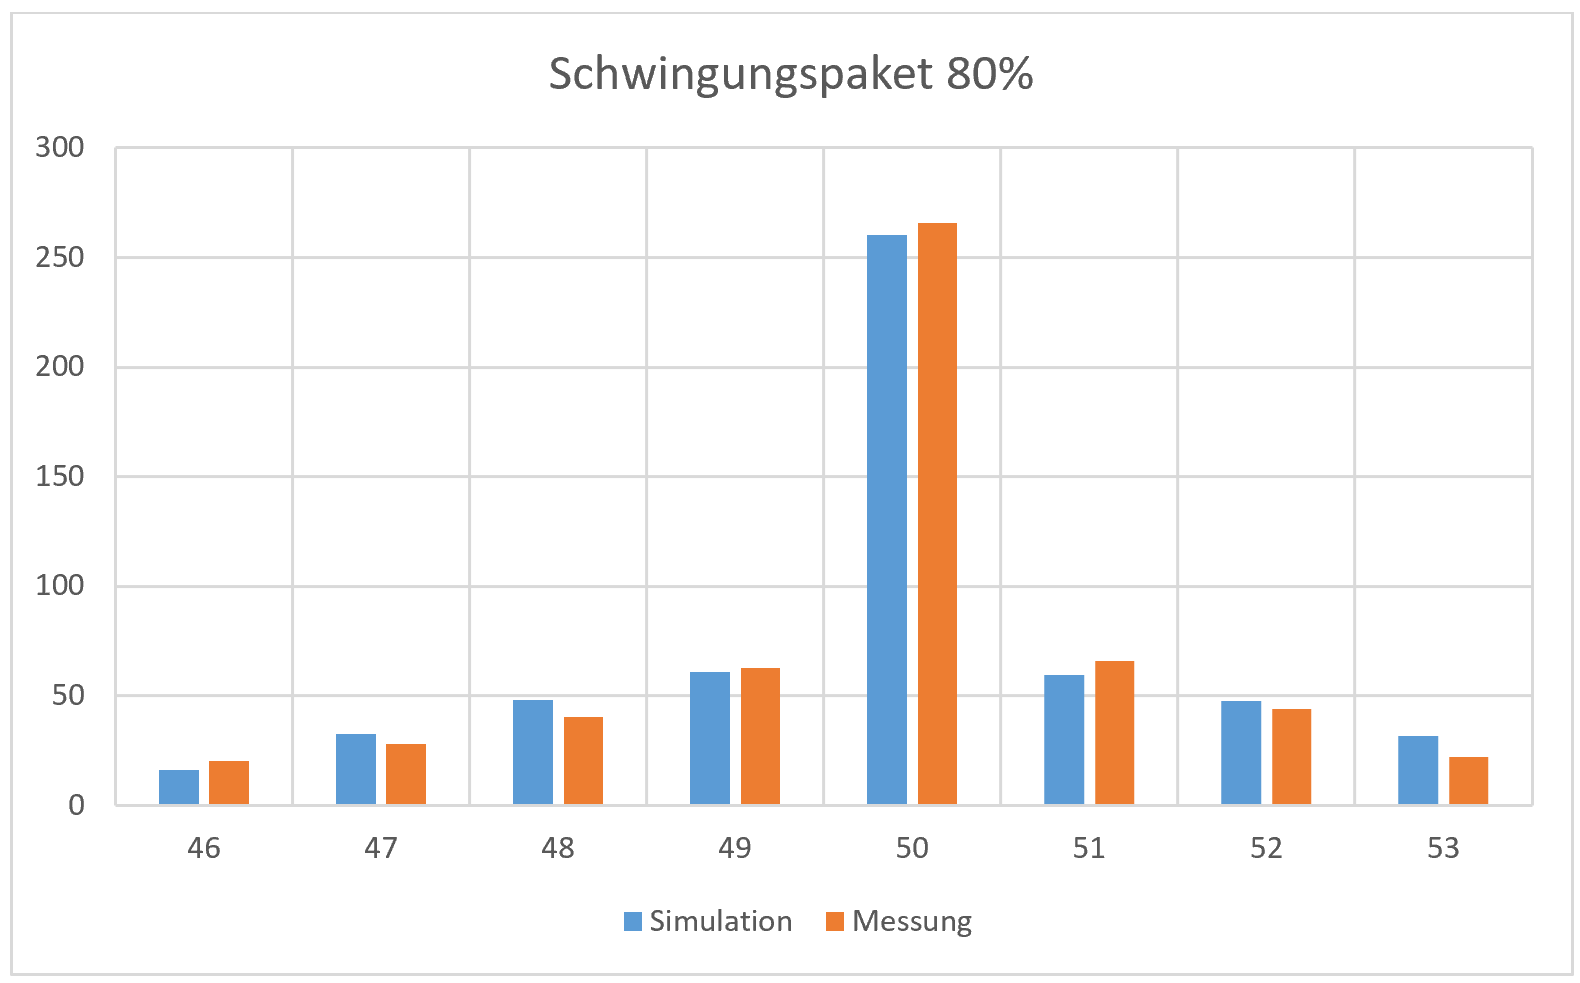
\includegraphics[width=\textwidth]{Vergleich_Mess_Sim_Schwing_80.png}	
		\caption{Vergleich Messung und Simulation mit Schwingungspaket mit einem Duty Cycle von 0.8}\label{fig:Vergleich_Schwing_80}
	\end{minipage}
	%
	\begin{minipage}[b]{0.4\textwidth}
		\centering
		\begin{tabular}{|l|l|l|}
			\hline
			\begin{tabular}[c]{@{}l@{}}Fre-\\ quenz\\ {[}Hz{]}\end{tabular} & \begin{tabular}[c]{@{}l@{}}Simu-\\ lation\\ {[}V{]}\end{tabular} & \begin{tabular}[c]{@{}l@{}}Mes\\ sung\\ {[}V{]}\end{tabular} \\ \hline
			46                                                              & 16.335                                                           & 20.173                                                       \\ \hline
			47                                                              & 32.649                                                           & 28.26                                                        \\ \hline
			48                                                              & 47.944                                                           & 40.576                                                       \\ \hline
			49                                                              & 61.08                                                            & 62.694                                                       \\ \hline
			50                                                              & 260.212                                                          & 265.98                                                       \\ \hline
			51                                                              & 59.54                                                            & 65.7                                                         \\ \hline
			52                                                              & 47.781                                                           & 43.812                                                       \\ \hline
			53                                                              & 31.664                                                           & 21.939                                                       \\ \hline
		\end{tabular}
		\caption{Vergleich Messung und Simulation mit Schwingungspaket mit einem Duty Cycle von 0.8}\label{tab:Vergleich_Schwing_80}
	\end{minipage}
\end{figure}



\newpage
\subsubsection*{Hartes Auf- und Absteuern}\label{sec:Vergleich_Mess_Sim_hart_AufAb}
\begin{figure}[ht!]
	\begin{minipage}[b]{0.59\textwidth}
		\centering
		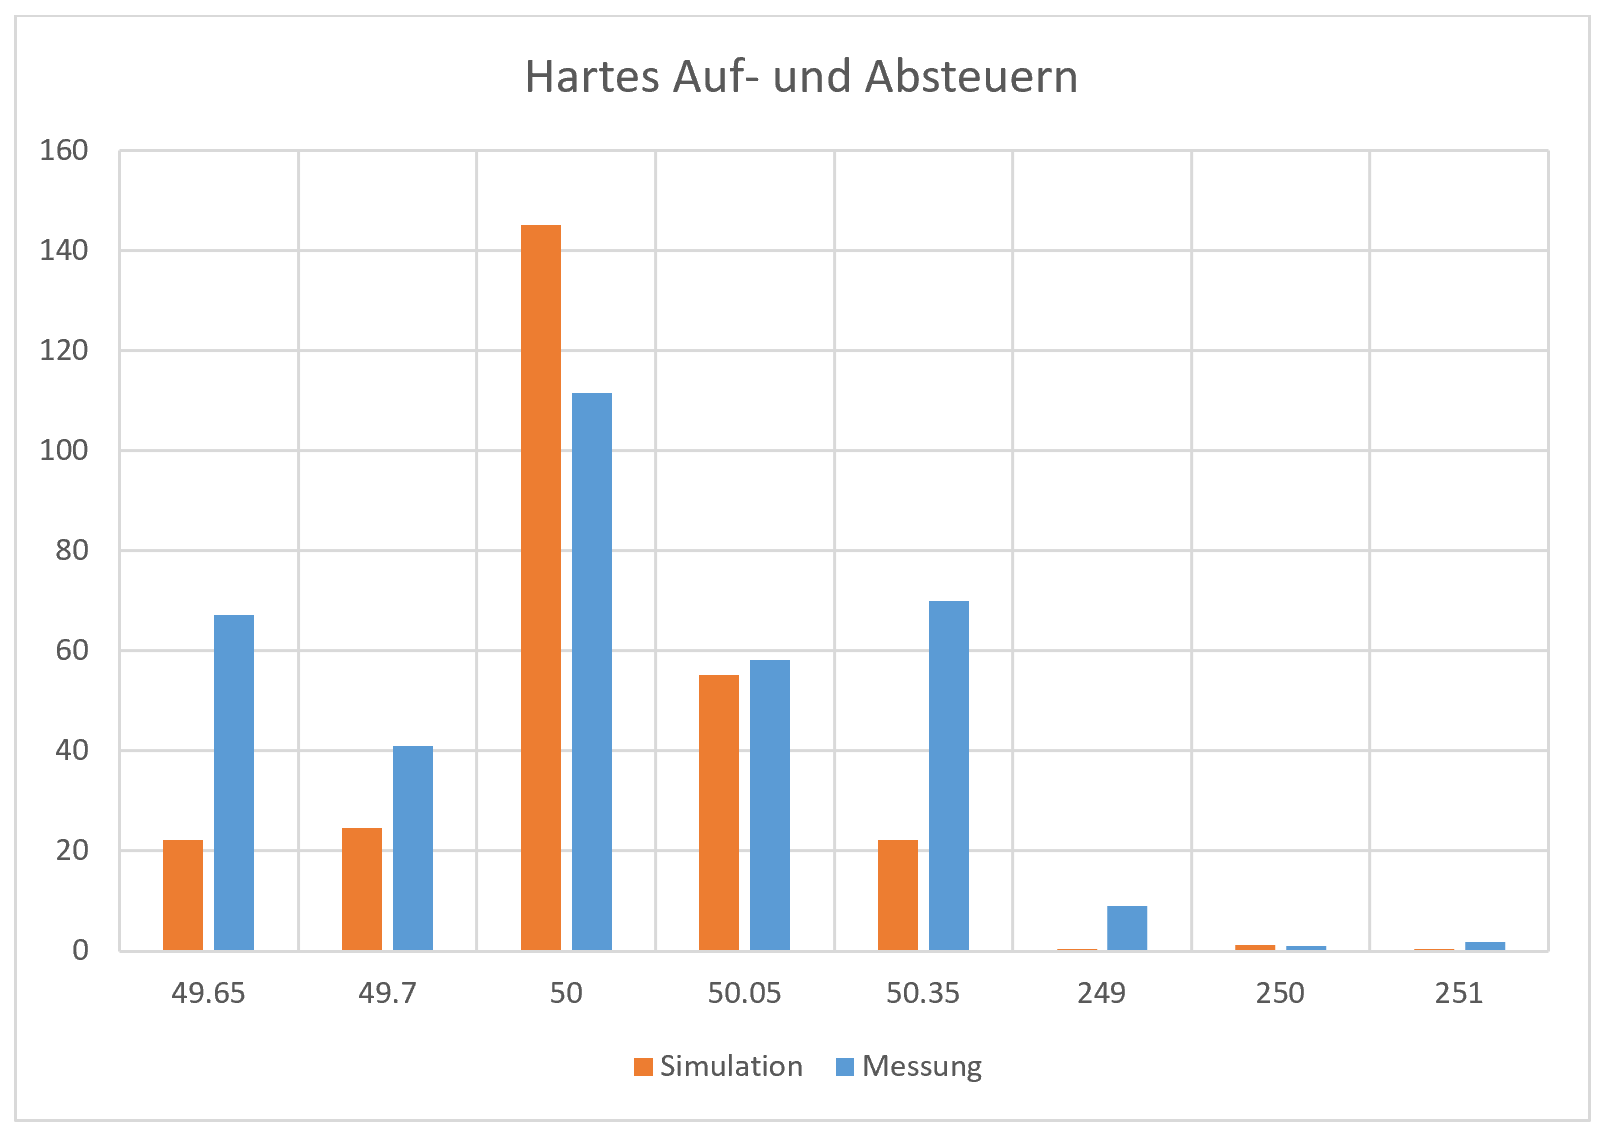
\includegraphics[width=\textwidth]{Vergleich_Mess_Sim_hart_AufAb.png}	
		\caption{Vergleich Messung und Simulation mit hartem Auf- und Absteuern}\label{fig:Vergleich_hart_AufAb}
	\end{minipage}
	%
	\begin{minipage}[b]{0.4\textwidth}
		\centering
		\begin{tabular}{|l|l|l|}
			\hline
			\begin{tabular}[c]{@{}l@{}}Fre-\\ quenz\\ {[}Hz{]}\end{tabular} & \begin{tabular}[c]{@{}l@{}}Simu-\\ lation\\ {[}V{]}\end{tabular} & \begin{tabular}[c]{@{}l@{}}Mes-\\ sung\\ {[}V{]}\end{tabular} \\ \hline
			49.65                                                           & 22.167                                                           & 67.126                                                        \\ \hline
			49.7                                                            & 24.504                                                           & 40.959                                                        \\ \hline
			50                                                              & 145.271                                                          & 11.676                                                        \\ \hline
			50.05                                                           & 55.113                                                           & 58.202                                                        \\ \hline
			50.35                                                           & 22.2                                                             & 70.065                                                        \\ \hline
			249                                                             & 0.473                                                            & 9.03                                                          \\ \hline
			250                                                             & 1.157                                                            & 0.108                                                         \\ \hline
			251                                                             & 0.29021                                                          & 1.53                                                          \\ \hline
		\end{tabular}
		\caption{Vergleich Messung und Simulation mit hartem Auf- und Absteuern}\label{tab:Vergleich_hart_AufAb}
	\end{minipage}
\end{figure}


\subsubsection*{Sanftes Auf- und Absteuern}\label{sec:Vergleich_Mess_Sim_sanft_AufAb}
\begin{figure}[ht!]
	\begin{minipage}[b]{0.59\textwidth}
		\centering
		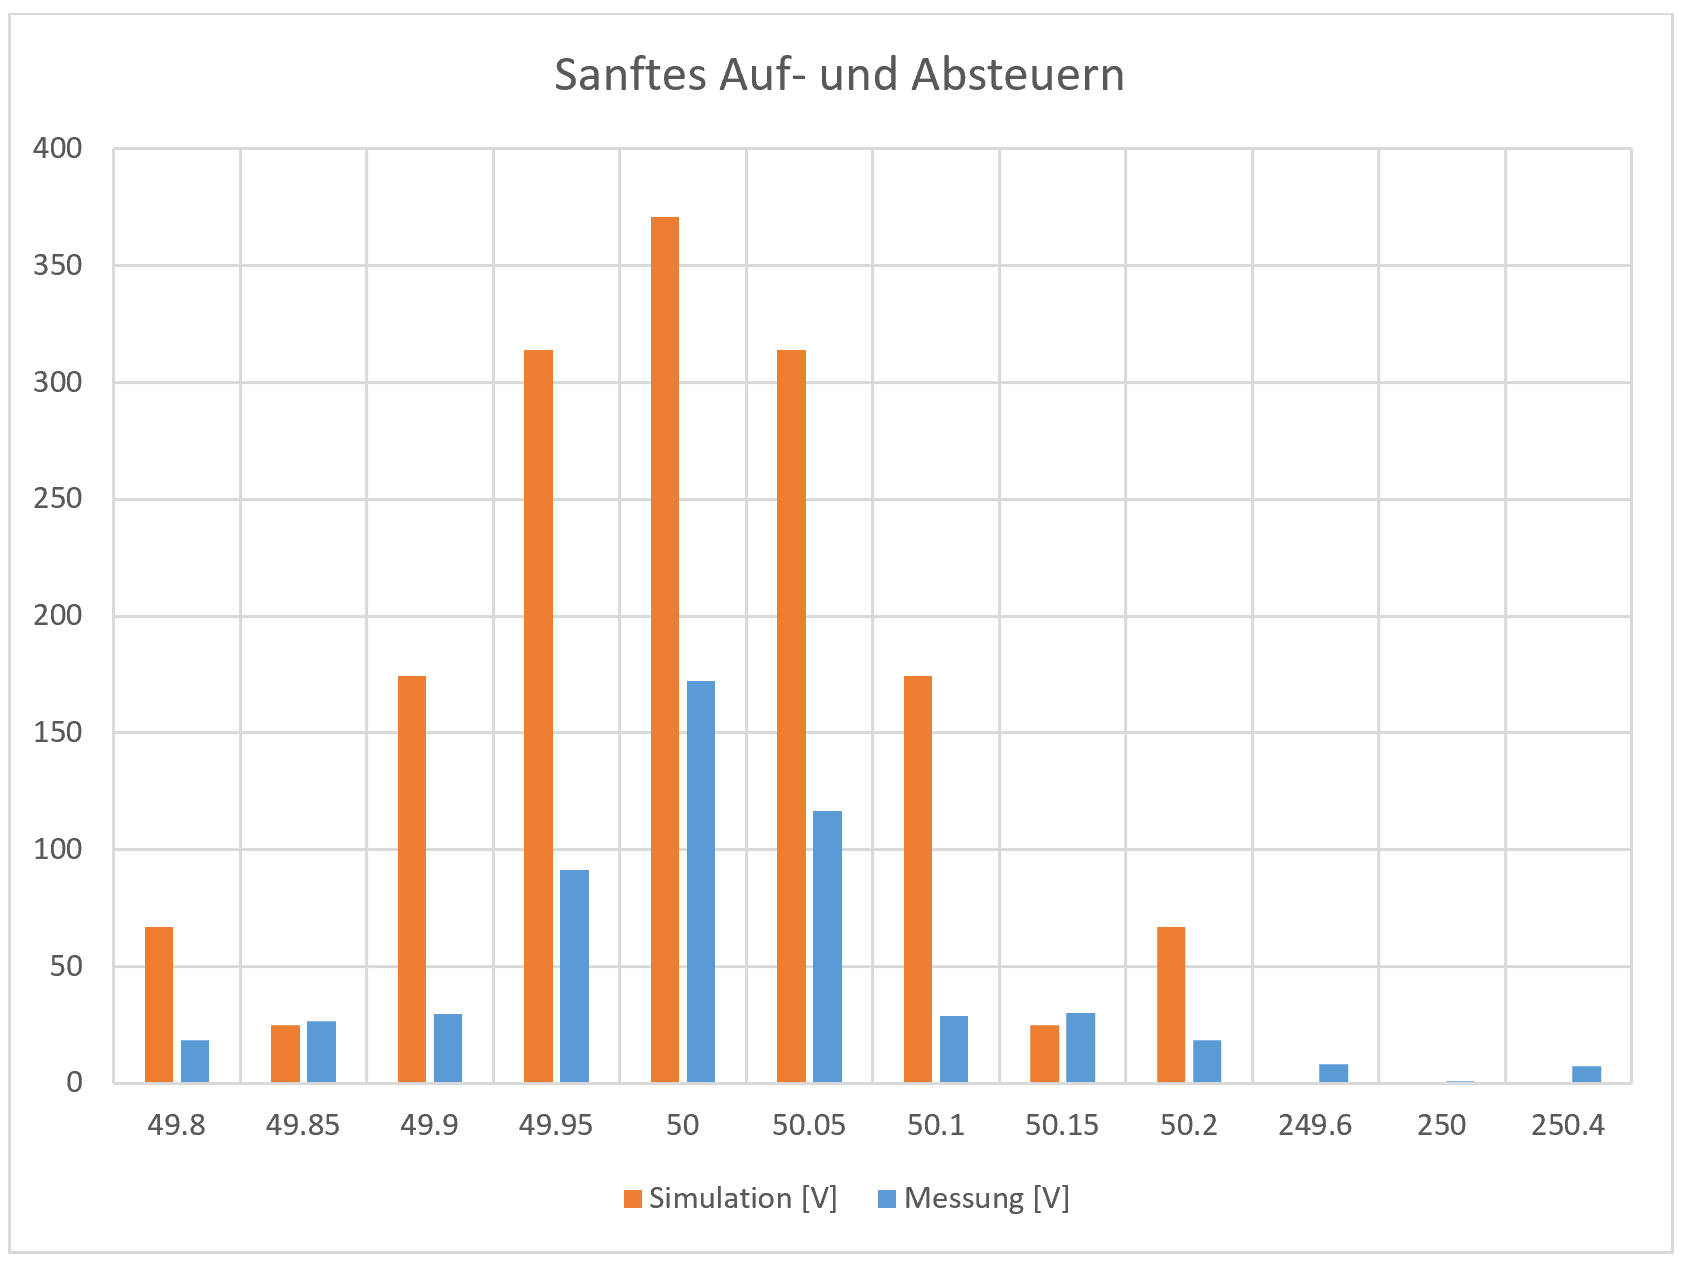
\includegraphics[width=\textwidth]{Vergleich_Mess_Sim_sanft_AufAb.png}	
		\caption{Vergleich Messung und Simulation mit sanftem Auf- und Absteuern}\label{fig:Vergleich_sanft_AufAb}
	\end{minipage}
	%
	\begin{minipage}[b]{0.4\textwidth}
		\centering
		\begin{tabular}{|l|l|l|}
			\hline
			\begin{tabular}[c]{@{}l@{}}Fre-\\ quenz\\ {[}Hz{]}\end{tabular} & \begin{tabular}[c]{@{}l@{}}Simu-\\ lation\\ {[}V{]}\end{tabular} & \begin{tabular}[c]{@{}l@{}}Mes-\\ sung\\ {[}V{]}\end{tabular} \\ \hline
			49.8               & 66.953             & 18.522          \\ \hline
			49.85              & 24.870             & 26.576          \\ \hline
			49.9               & 174.378            & 29.507          \\ \hline
			49.95              & 314.127            & 91.266          \\ \hline
			50                 & 370.962            & 172.241         \\ \hline
			50.05              & 314.051            & 116.719         \\ \hline
			50.1               & 174.266            & 28.629          \\ \hline
			50.15              & 24.871             & 30.076          \\ \hline
			50.2               & 66.83              & 18.72           \\ \hline
			249.6              & 0.188              & 8.158           \\ \hline
			250                & 0.4967             & 1.158           \\ \hline
			250.4              & 0.445              & 7.466           \\ \hline
		\end{tabular}
		\caption{Vergleich Messung und Simulation mit sanftem Auf- und Absteuern}\label{tab:Vergleich_sanft_AufAb}
	\end{minipage}
\end{figure}


\end{appendix}


